\chapter{DAQ readout testing}
\textit{In this Chapter, I present the initial results of the tracker DAQ commissioning. Before reading out the detector, 
    it was necessary to understand the readout process. This Chapter is divided into three sections: the first relates 
    to the validation of ROC readout through Monte Carlo simulation, subsequently, I will discuss the initial and primitive tracker panel data quality monitoring, 
    and in the third part, I will address high-rate software testing.XXX}
    
  \section{Description of teststand setup}\label{des}
    The tracker test stand, called TS1, shown in Figure \ref{fig:TS1}, included one DRAC card, \ref{DRAC}, connected via an optical fiber
    to the DTC installed in the DAQ computer, called mu2edaq09. The teststand included 96 channels in total.
    The ROC, \ref{ROC}, could be operated in two different data readout modes:
    \begin{itemize}
    \item  First mode: the ROC was emulating the data itself without reading FPGAs (a pattern readout mode);
    \item  Second mode: the ROC was reading digi FPGAs.
    \end{itemize}
    \begin{figure}[!h]
        \centering
        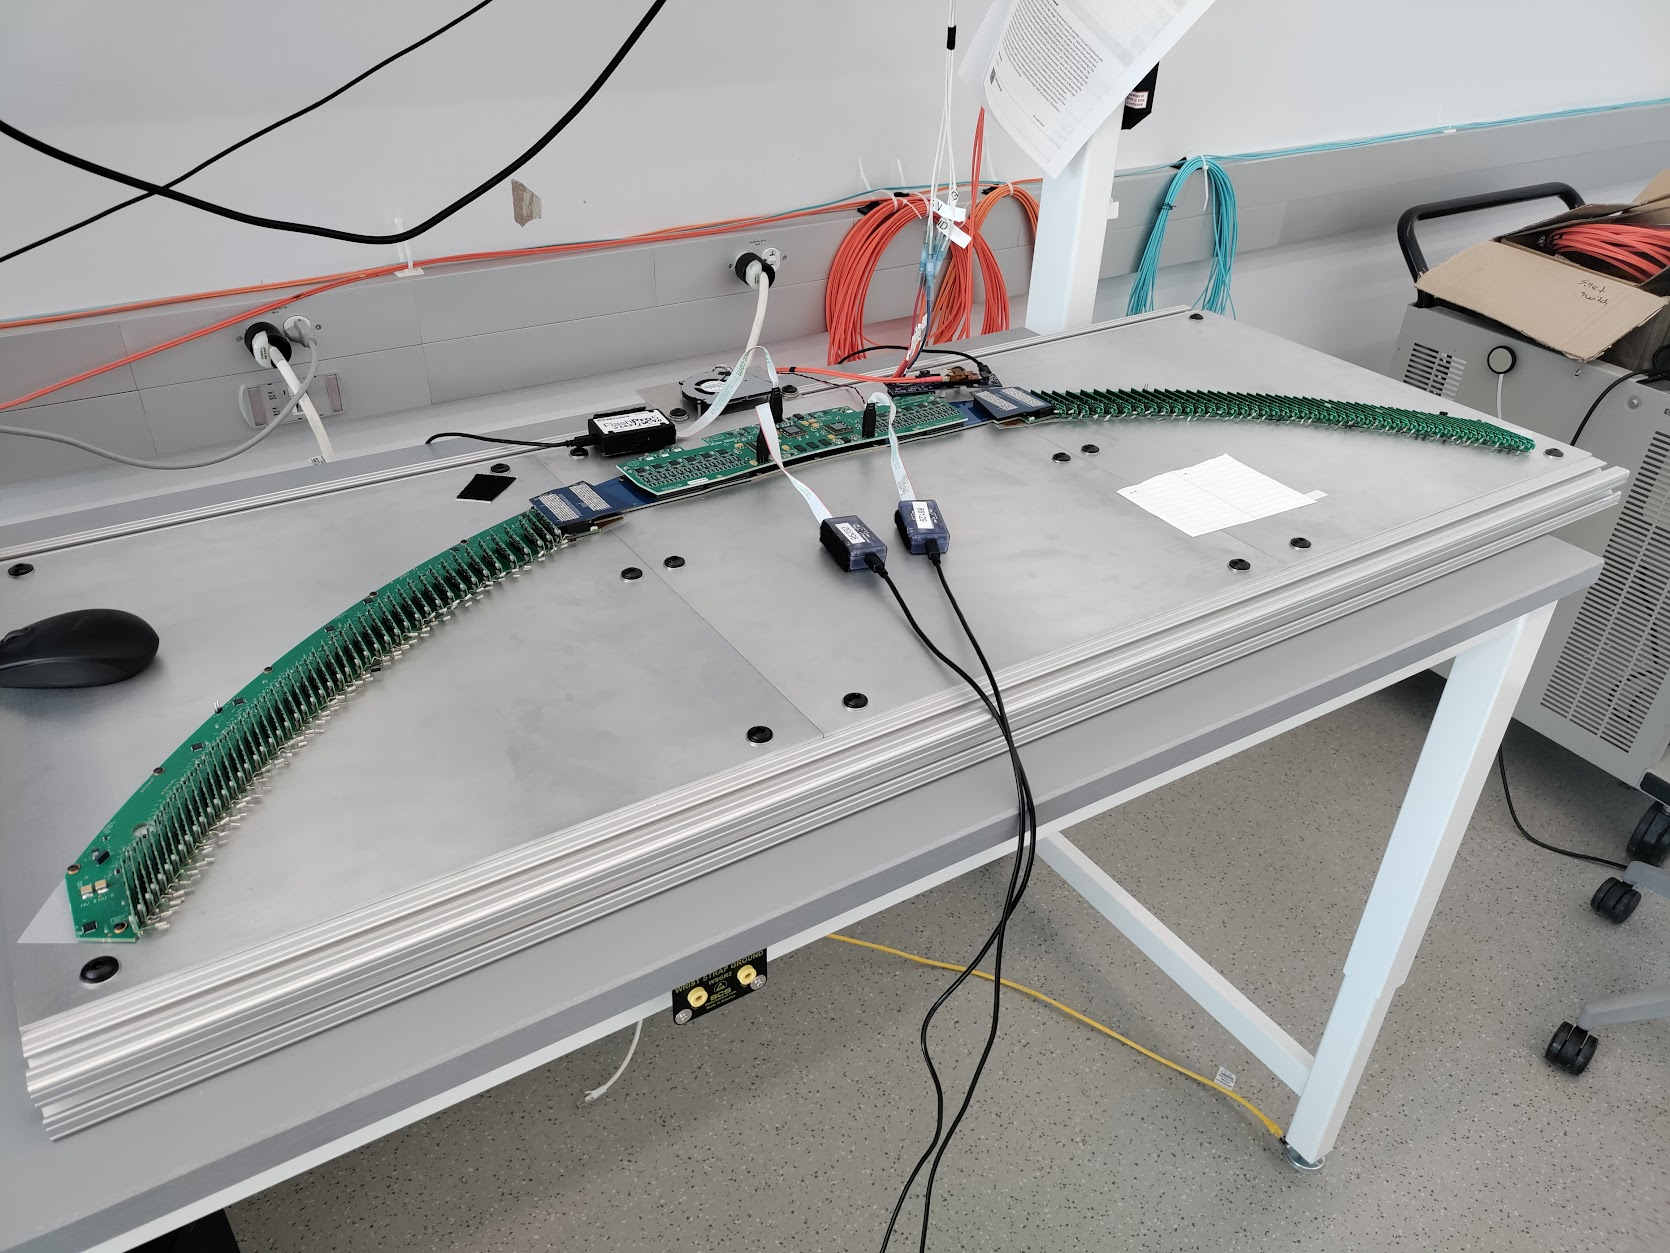
\includegraphics[width =0.55\textwidth]{figures/jpg/IMG_20240219_090538.jpg}
        \caption{The tracker test stand, TS1, featuring one DRAC card linked via optical fiber to the DTC in the DAQ computer (mu2edaq09). The setup includes a total of 96 channels.}
        \label{fig:TS1}
        \end{figure}
    Most of the data were taken operating in the second mode, with digi FPGAs, pulsed by their internal pulsers.
    The pulser has two different frequencies,  31.29 MHz/(2$^7$+1), or approximately 250 kHz, 
    and 31.29 MHz/(2$^9$+1), or approximately 60 kHz.
    Event window is the time interval between two heartbeats (HB's). 
    A timing diagram of a single channel readout is shown in Figure \ref{fig:3}.
    Pulses, separated by $T_{gen}=1/f_{gen}$, where $f_{gen}$ is the generator frequency
    are represented by gray triangles.
    The event window, with the width of $T_{EW}$, that represents the distance between the proton pulses, 
    was varied from 700 ns to 50 $\mu$s, to test the system and to increase flexibility during tests, but during Mu2e data taking it will be approximately 1.7 $\mu$s. 
    The ROC firmware has an internal hit buffer which stores up to 255 hits.
    Depending on $T_{gen}$ and $T_{EW}$, the data taking can proceed in two different
    scenarios:
    \begin{itemize}
    \item
      The event window is large enough , so the total number of generated hits is greater than 255. In this case
      the ROC hit buffer always gets filled up, and only the first 255 hits are read out;
    \item
      The total number of hits within the event window is less than 255.
      In this case the ROC hit buffer doesn't get filled up and the total number of hits may vary from one event to another.
    \end{itemize}
    Each digi FPGA has its own pulse generator and the pulse sequences from the two
    generators are offset with respect to each other by a time interval $\Delta t$. 
    The offset is constant for as long as the DRAC board is powered up and varies randomly between 0 and $T_{gen}$ when DRAC is powercycled. 
    The timing of the readout is uncorrelated with the generator timing sequences, 
    so the number of pulses within the readout window can vary from one event to another, as shown 
    in Figure \ref{fig:3}. Relative timing offsets of the channels within the same FPGA are of the order of a few ns. The channel readout sequence is fixed.
    \begin{figure}[!h]
    \centering
    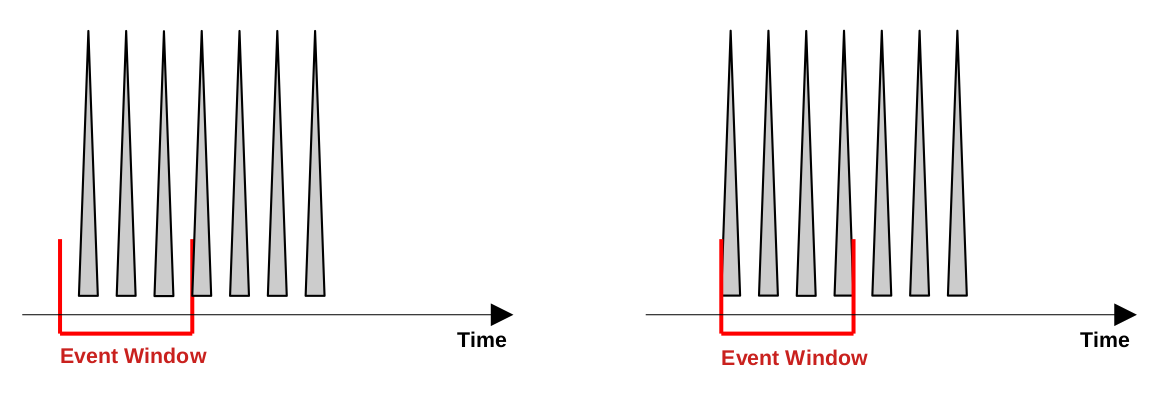
\includegraphics[width =0.85\textwidth]{figures/png/finalimg.png}
    \caption{Graphic illustration of pulses in an event window.}
    \label{fig:3}
    \end{figure}
    For the testing described in \ref{MonteCarlo}, only one ROC connected to the DTC was used. However, for the testing described in \ref{dqm}, two ROCs connected to one DTC were also used.
    %The data taking has been performed $\mu$sing OTSDAQ+ARTDAQ software, and for each run the output data have been stored in an art file moved to {\bf /exp/mu2e/data/projects/tracker/vst} area mounted on Mu2e central platforms.
\section{Validation of ROC readout through Monte Carlo}
%%%%%%%%%%%%%%%%%%%%%%%%%%%%%%%%%%%%%%%%%%%%%%%%%%%%%%%%%%%%%%%%%%%%%%%%%%%%%%
\subsection{ROC Monte Carlo simulation}\label{MonteCarlo}
 
The ROC readout logic is purely digital, so the readout process can be simulated. 
The logic of the simulation is as follows. The simulated parameters for each event are the number of hits in each channel
and the total number of readout hits. In the following sections, we call $occupancy$ the total number of hits
recorded in a given channel during the test run. Given that the total number of hits per event doesn't exceed 255, the simulation follows these steps:
\begin{itemize}
\item
  The event window starts at $t=0$s;
\item
  In a given FPGA, the timing of the first pulse is generated randomly from 0 to $T_{gen}$
  by sampling a uniform distribution;
\item
  The subsequent pulses are added, separated from each other by $T_{gen}$,
  until the absolute time
  of the next pulse is greater than $T_{EW}$;
\item
  In the readout part of the simulation, the pulses are read out following the readout sequence;
\item
  the readout ``continues'' until all simulated hits are included or
  the total number of read out hits reaches the maximum threshold of 255. 
\end{itemize}

The simulation also takes into account the offset between the two FPGA timing sequences and the 
individual channel-to-channel timing offsets. These delays were studied by comparing the real timing 
differences between channels, specifically between a channel and the reference (first readout) channel of that 
specific FPGA, channel 91 for the FPGA-1 and 94 for the second. Figures \ref{fig:delay1} and \ref{fig:delay2} 
shows an example of the fits of time differences between channels 91 and 0 in the FPGA-1, and 94 and 44 in the FPGA-2. 
The channel-to-channel delays are of the order of few ns. The histograms have been simply fitted with a Gaussian function 
to evaluate the mean delay for each channel. This procedure was repeated for all channels and the values were added to the Monte Carlo.
In the following sections, the results of the data collection are compared with the simulation.

  \begin{figure}[!h]
          \centering
      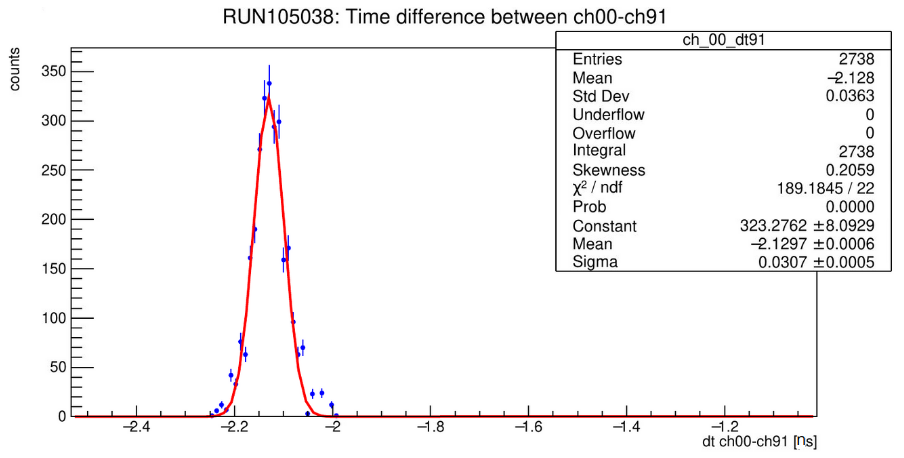
\includegraphics[width=0.7\textwidth]{figures/png/Screenshot from 2023-12-03 11-50-50.png}
      \caption{FPGA-1: histogram of the delay between channel 0 and the reference channel 91, the first to be readout.}
      \label{fig:delay1}
    \end{figure}
    \begin{figure}[!h]
          \centering
      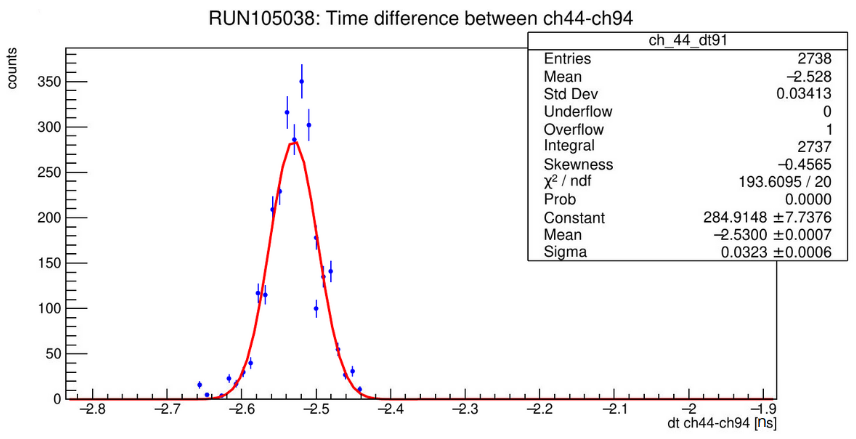
\includegraphics[width=0.7\textwidth]{figures/png/Screenshot from 2023-12-03 11-50-33.png}
      \caption{FPGA-2: histogram of the delay between channel 44 and the reference channel 94, the first to be readout.}
      \label{fig:delay2}
    \end{figure}
\subsection{``ROC buffer overflow'' mode}
In the ``ROC buffer overflow'' configuration, which will be referred to as RUN281, the event window size is 50 $\mu$s
and the pulser rate is 60 kHz.
\subsubsection{Hit timing and occupancy}\label{over}
The first distributions to look at are the time distributions of hits in 
different channels and the distribution of the total number of hits
in a given channel (occupancy) as a function of the channel number.
The timing distributions of hits in channel 0 of the FPGA-1
and in channel 2 of the FPGA-2 are shown in Figure \ref{fig:1}.
The top distribution is, as expected, uniform, however the right one looks
less trivial.
\begin{figure}[!h]
  \begin{subfigure}[b]{\textwidth}
      \centering
      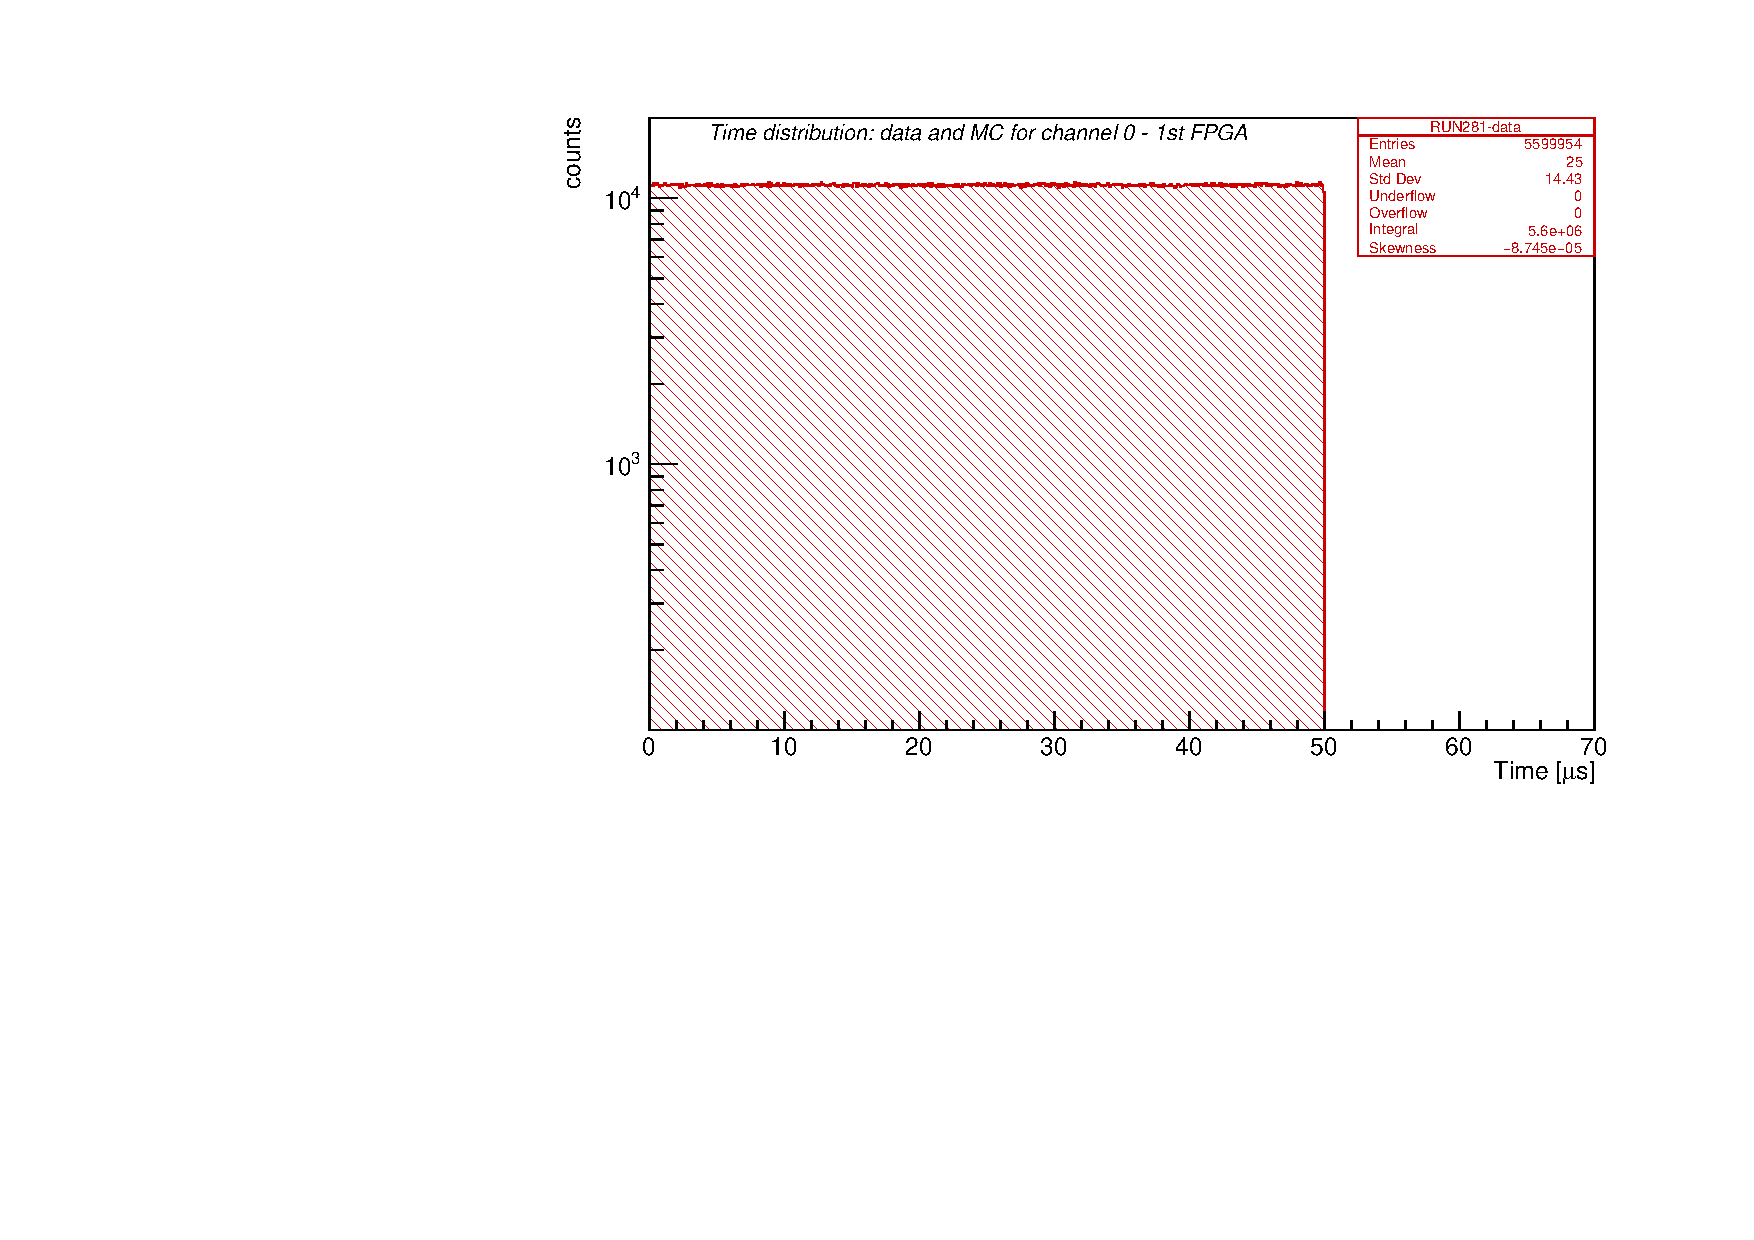
\includegraphics[width=0.7\textwidth]{figures/pdf/figure_00007_timedistr_roc_simulation_ch0_281.pdf}
      \label{fig:t1}
  \end{subfigure}
\\
  \begin{subfigure}[b]{\textwidth}
      \centering
      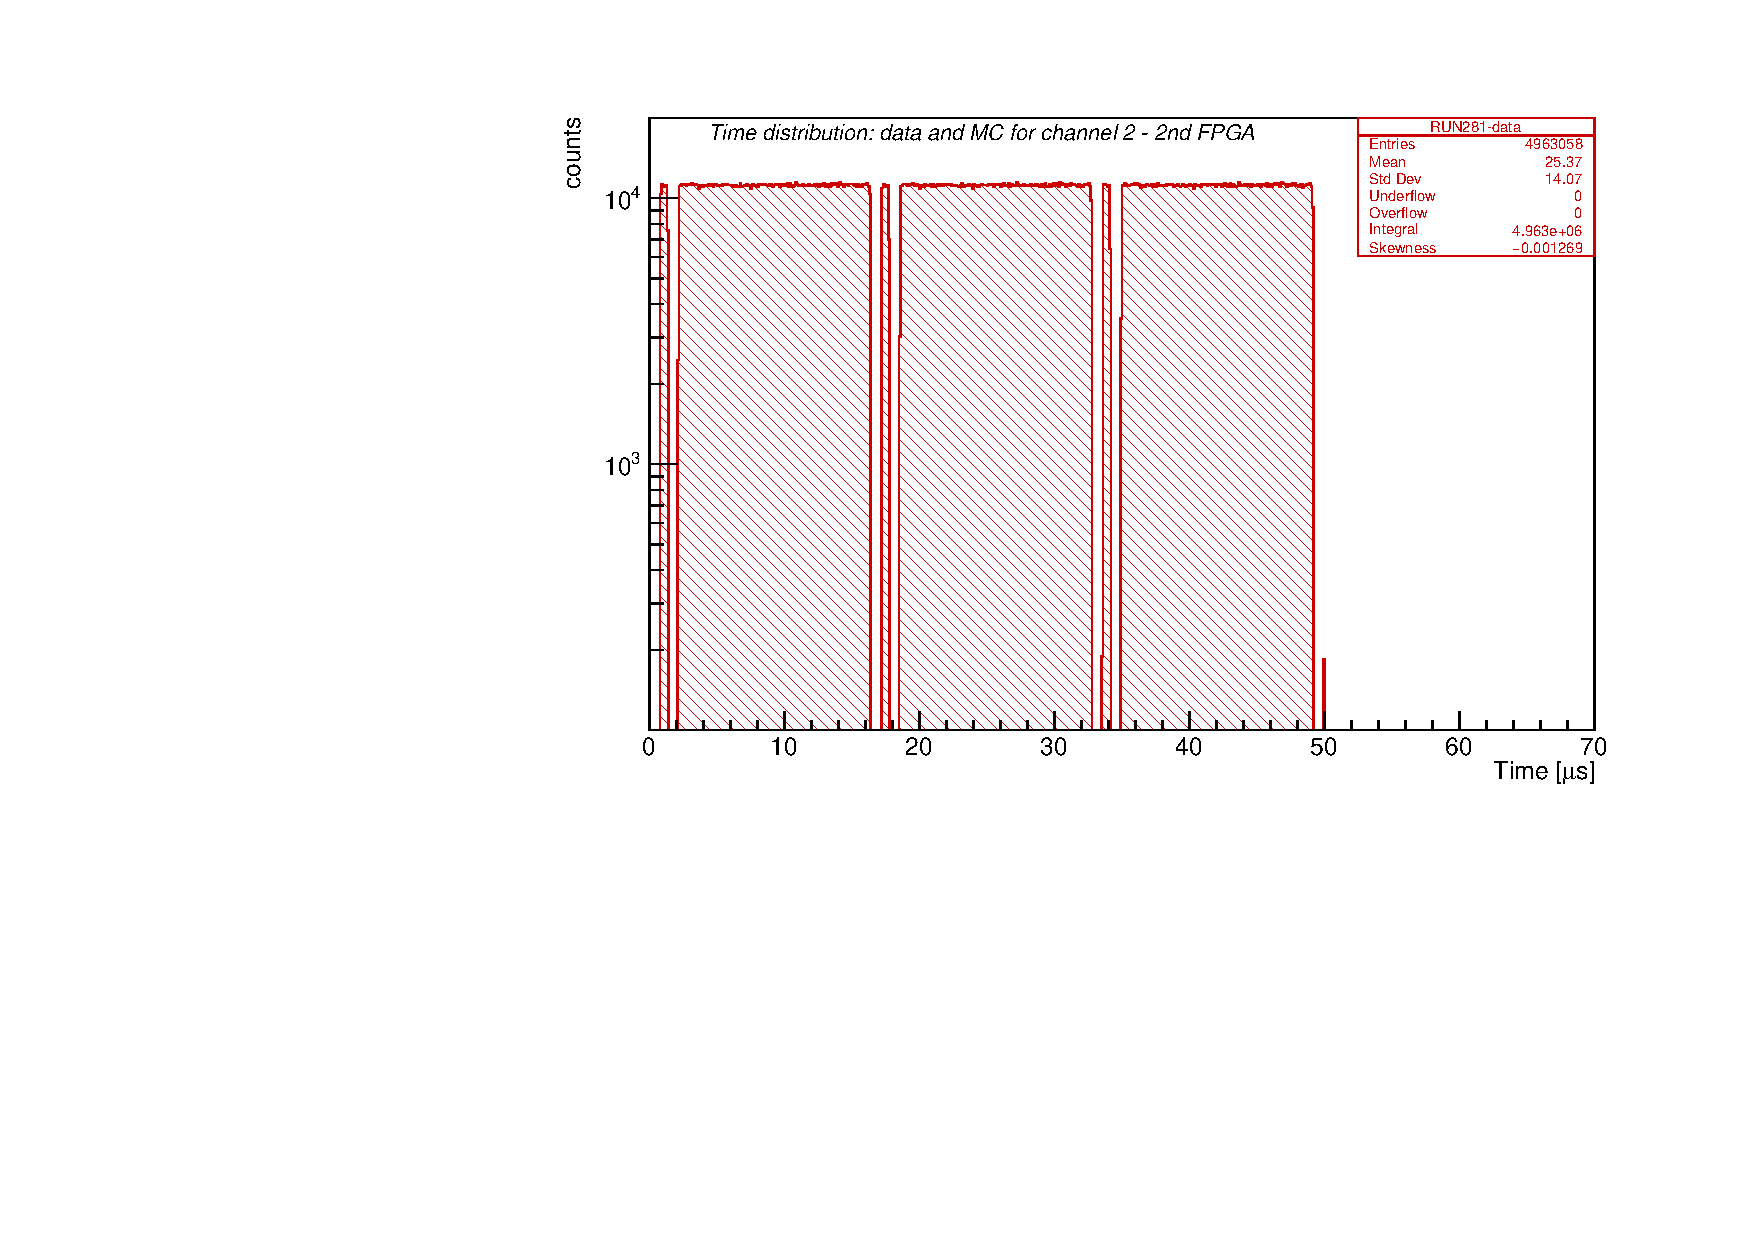
\includegraphics[width=0.7\textwidth]{figures/pdf/figure_00003_timedistr_roc_simulation_ch2_281.pdf}
      \label{fig:t2}
  \end{subfigure}
     \caption{(Top): time distribution of hits in the channel 0 in the FPGA-1.
     (Bottom): time distribution of hits in the channel 2 in the FPGA-2.}
     \label{fig:1}
\end{figure}
The distributions in Figure \ref{fig:1} are easier to understand by looking at the occupancy plot in Figure \ref{fig:2} (Top).
The channel ordering in this plot corresponds to the readout order.
Channels in the beginning of the readout sequence always have all their hits read out,
  however that is not true for the channels in the end of the readout sequence.
  \begin{figure}[!h]
    \begin{subfigure}[b]{\textwidth}
        \centering
        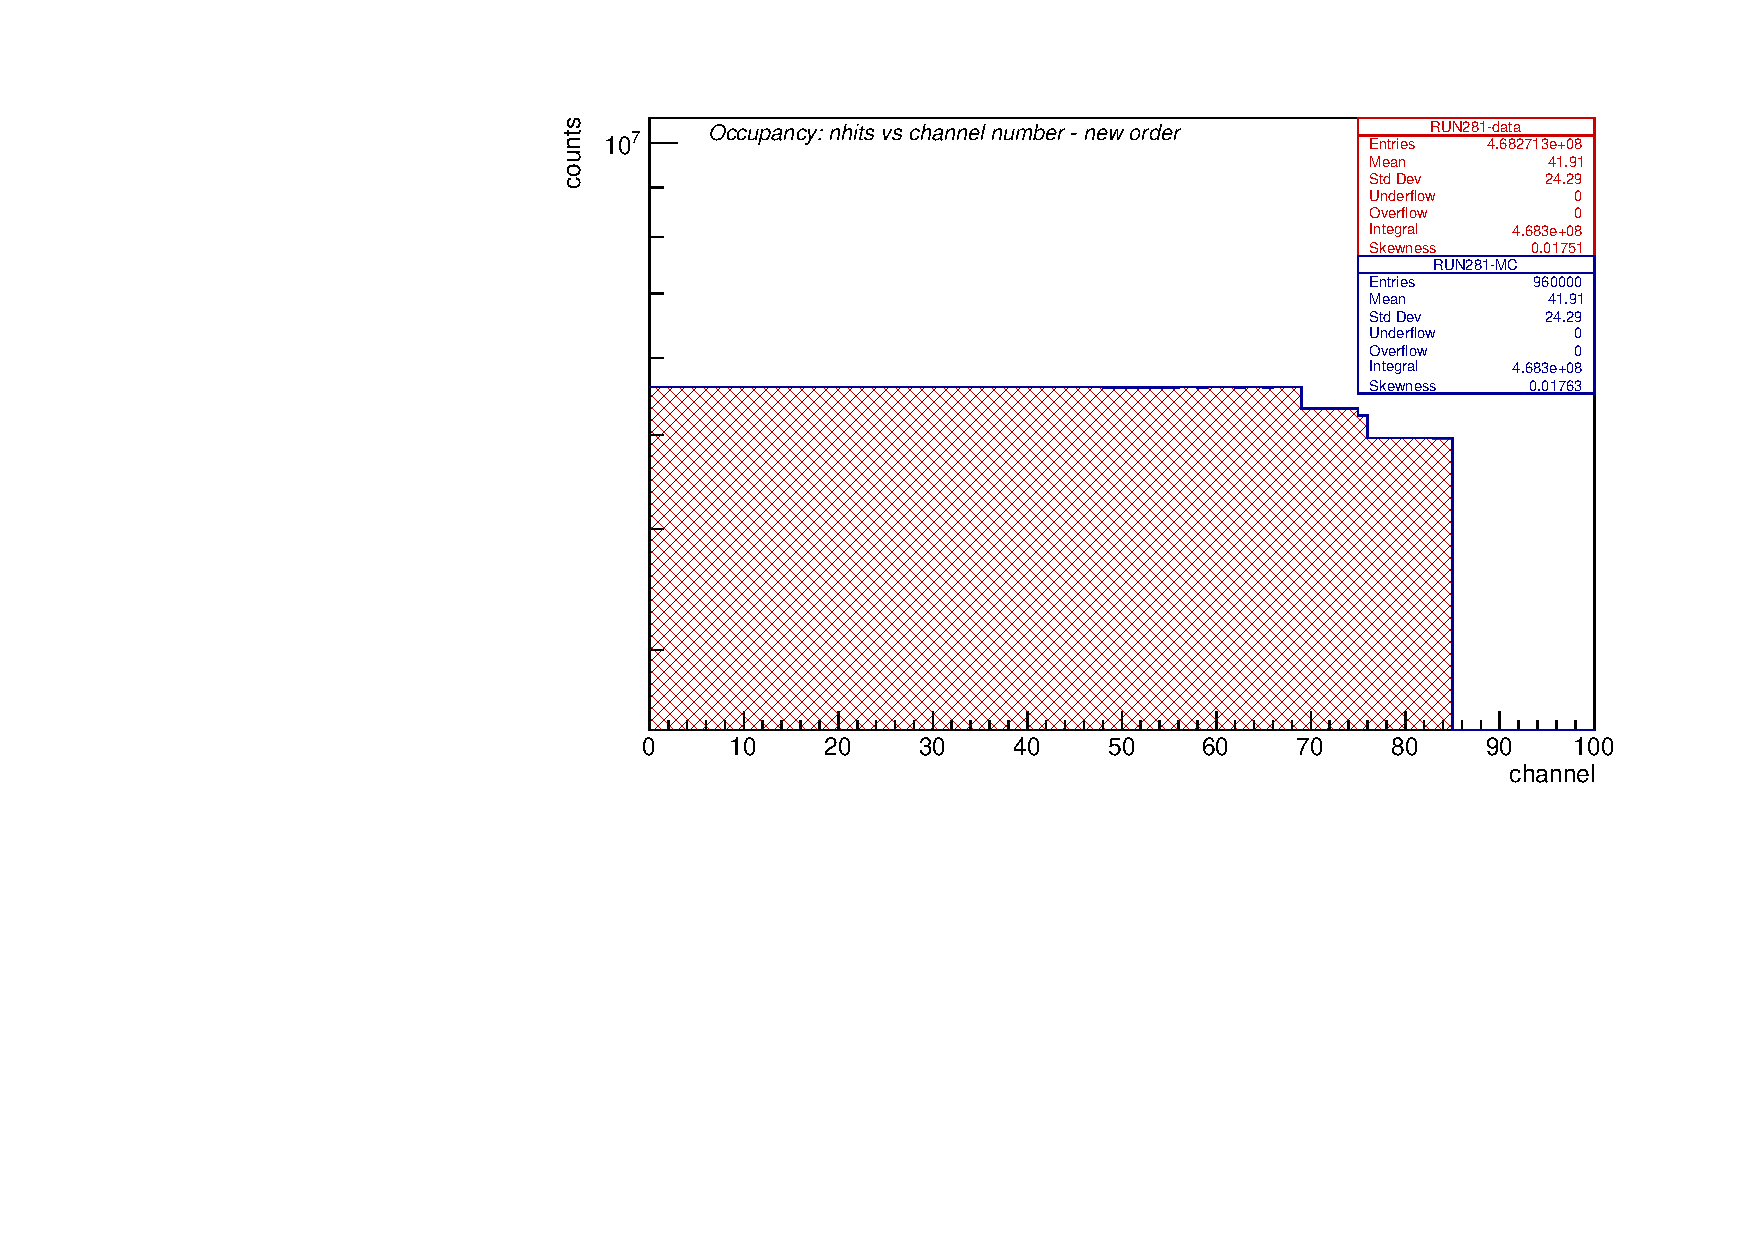
\includegraphics[width=0.7\textwidth]{figures/pdf/figure_00004_nhitsvschannel_roc_simulation_281.pdf}
        \label{fig:tt1}
    \end{subfigure}
  \\
    \begin{subfigure}[b]{\textwidth}
        \centering
        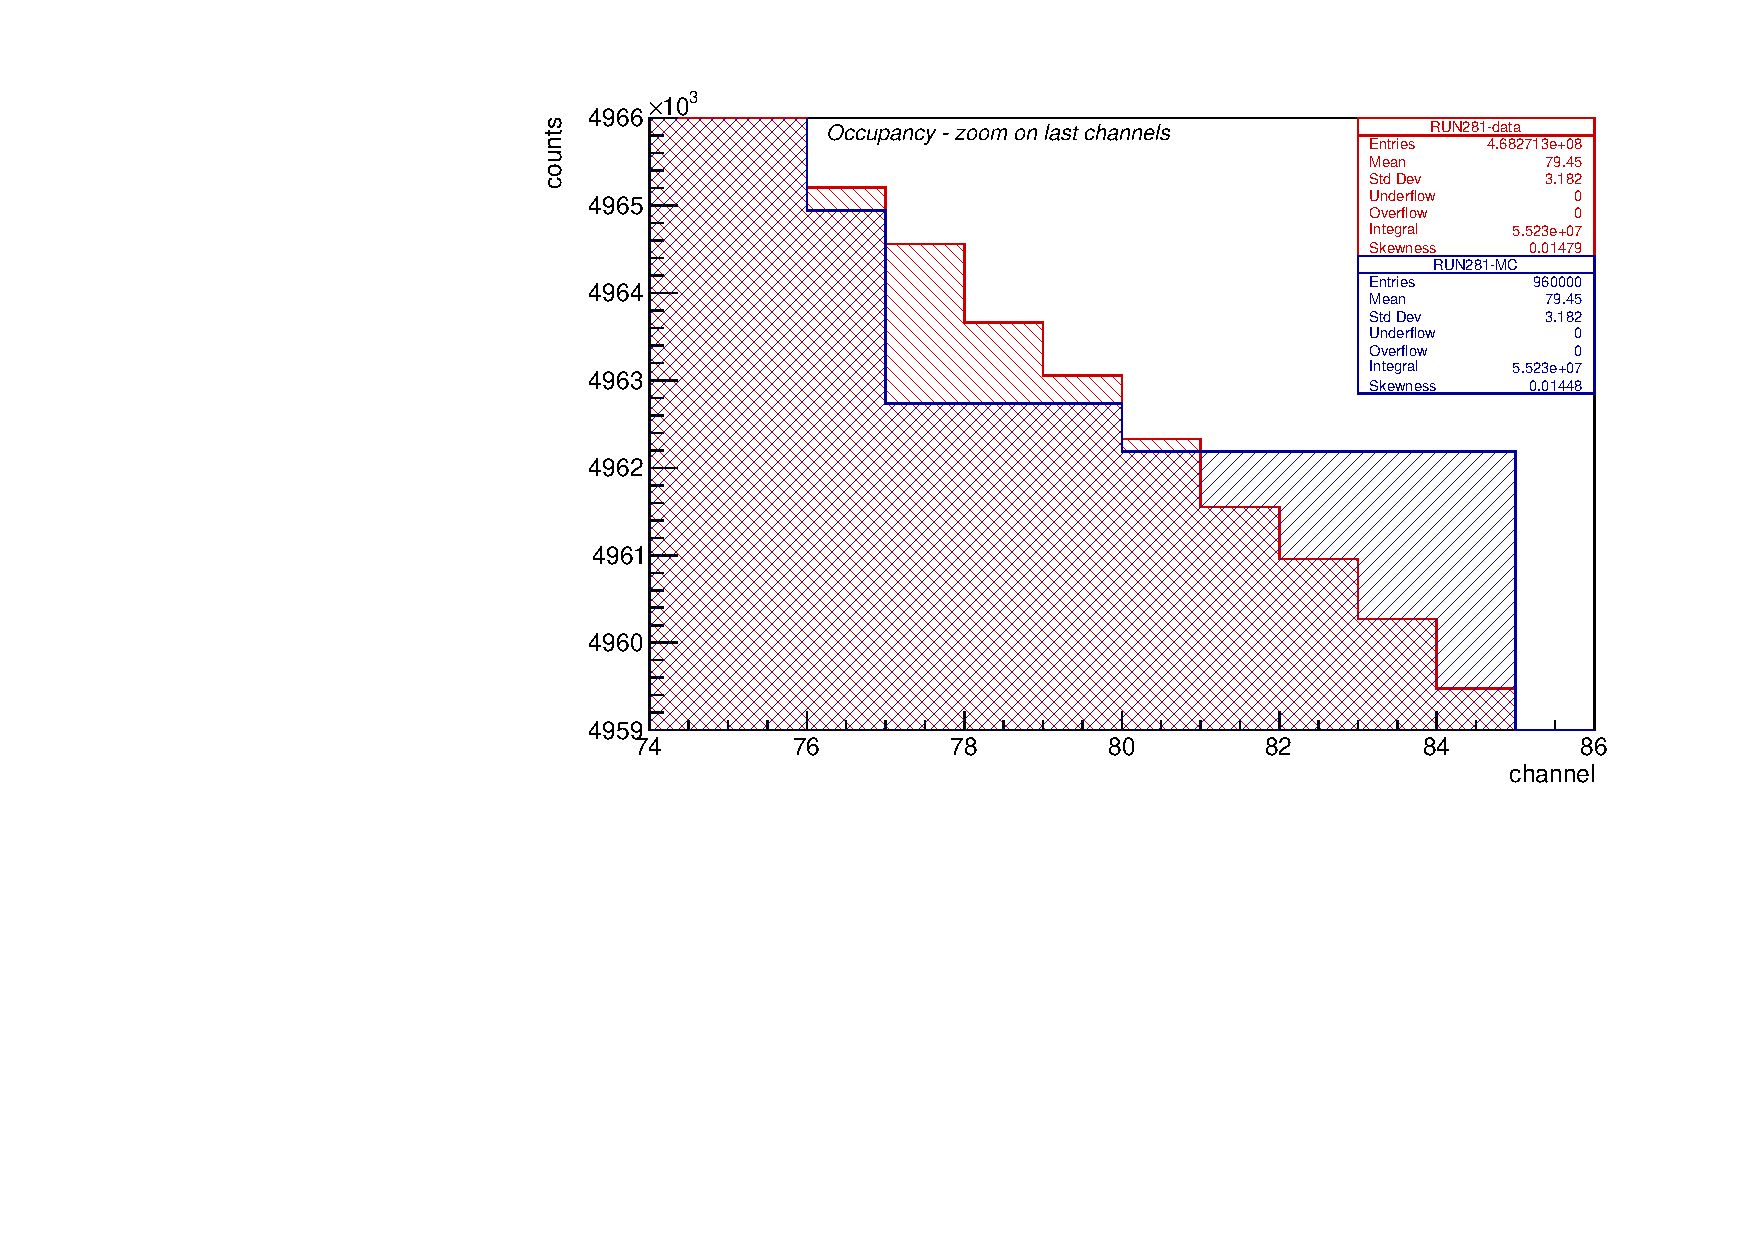
\includegraphics[width=0.7\textwidth]{figures/pdf/figure_00014_nhitsvschannel_roc_simulation_281.pdf}
        \label{fig:tt2}
    \end{subfigure}
       \caption{(Top): number of hits versus the channel number. The channels are numbered in the readout order.
       (Bottom): zoom on the last channels in the readout sequence. The data and MC distributions
       differ from each other by $\sim$ 10$^{-3}$.}
       \label{fig:2}
  \end{figure}


Figure \ref{fig:66} shows the distribution of the number of hits in channel 0.
For the event window of 50 $\mu$s and the time between the pulses of 16 $\mu$s,
the number of hits could be 3 or 4,
depending on the timing offset of a given readout window with respect to the generated timing sequence.
This distribution plays a key role in understanding of the occupancy plot.
\begin{figure}[!h]
\centering
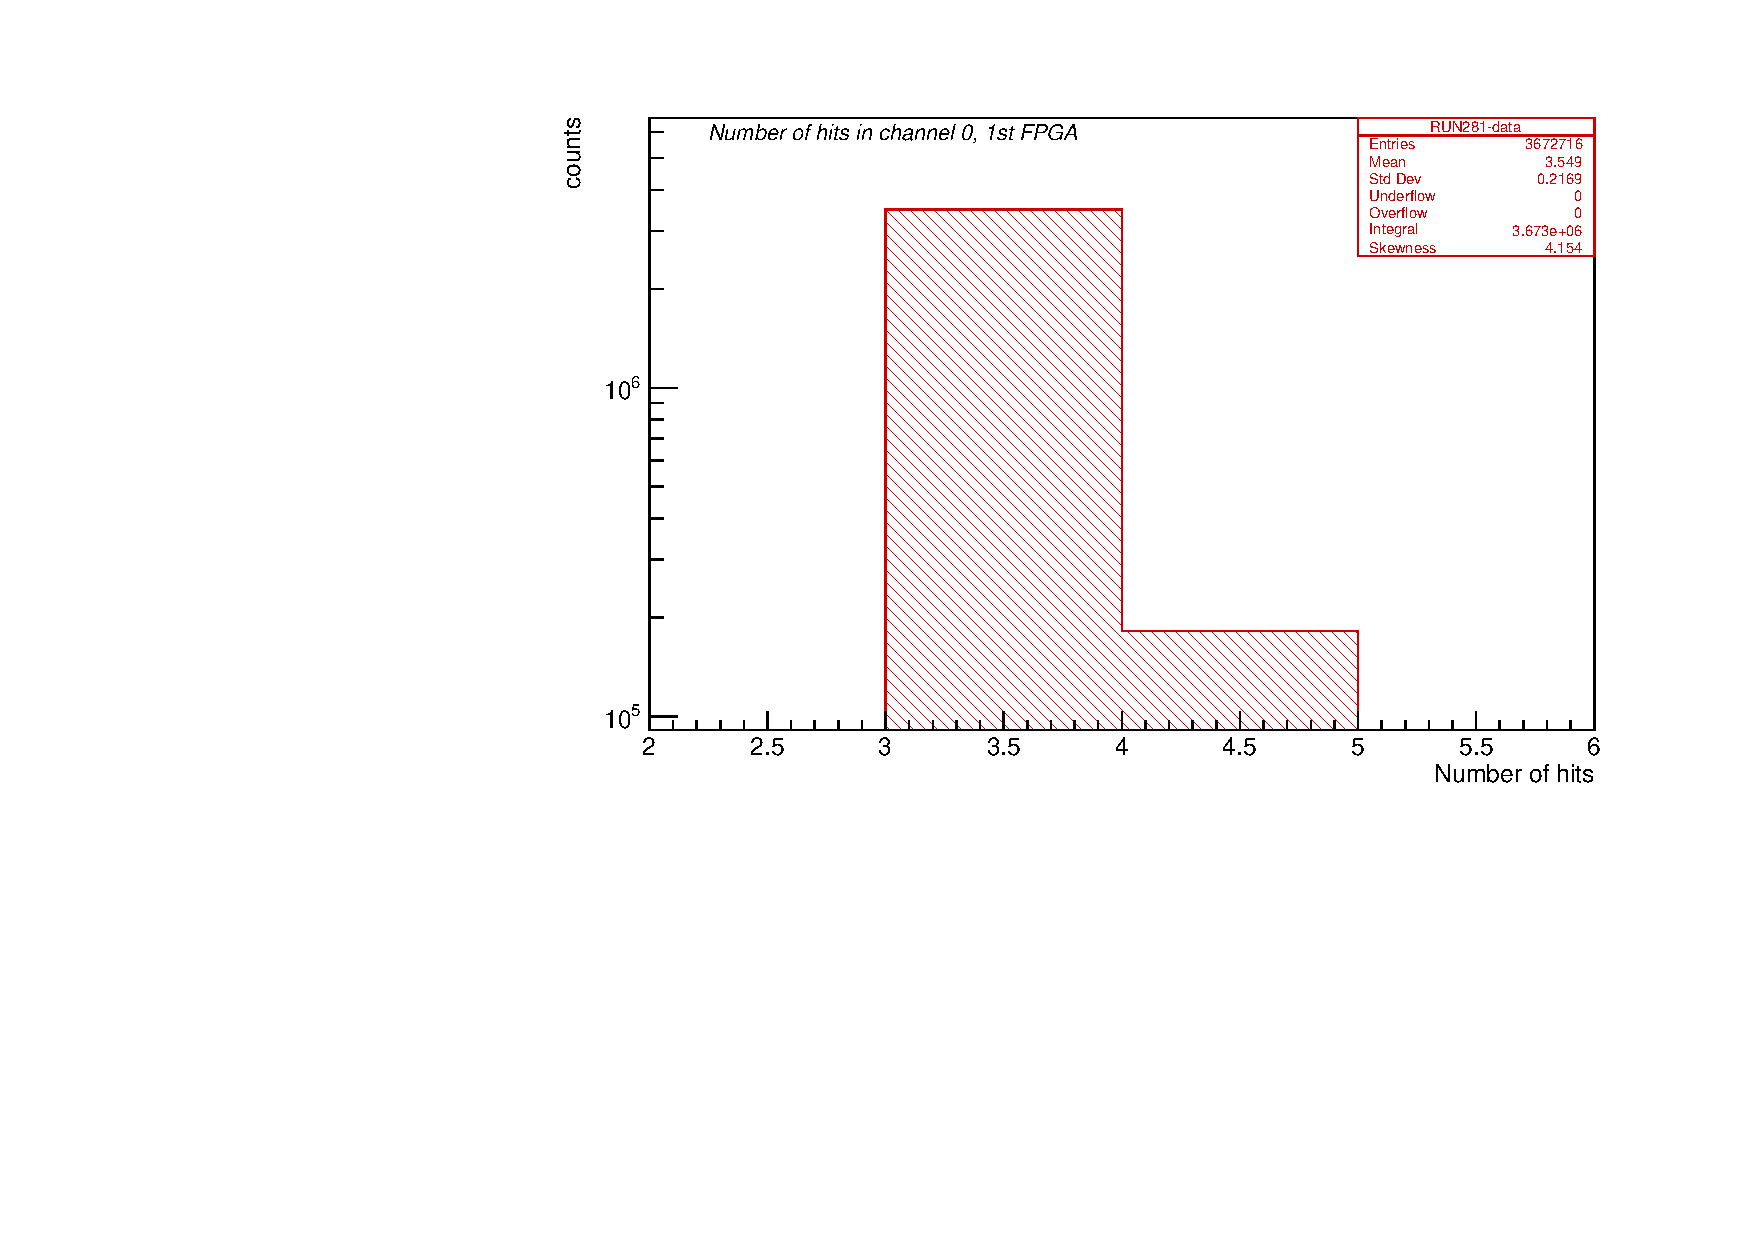
\includegraphics[width =0.7\textwidth]{figures/pdf/figure_00066_nhits_ch00_run281.pdf}
\caption{
  The distribution of the number of hits in the channel 0 of the first digi FPGA (RUN281).
}
\label{fig:66}
\end{figure}

In the distribution shown in Figure \ref{fig:2} (Top),
the first 68 channels are the ones with 4 hits per channel in the FPGA-1
and three hits per channel in the FPGA-2, 
resulting in the total of 255 hits.
The second plateau extending from 68 to 75 corresponds to the channels
with 3 hits per channel in the FPGA-1 and 4 hits per channel in the second one.
  The ``dent'' in the end of the second plateau is due to the fact that the 48 channels of the FPGA-1
  yield 144 hits, so the FPGA-2 contributes 111 hits. The first 27 channels of the FPGA-2 contribute
  4 hits per channel each, but as 111 is not an integer of 4, the three hits from channel 28 in the readout sequence
  fill up the total ROC buffer of 255 hits.
There is a big step at the end of this plateau, because if we count the number of hits
in the FPGA-1 we get 144, so in the FPGA-2 we have 111 hits in total,
due to the fact that the maximum number of hits in total is 255.
111 is not divisible by 4, so the first 27 channels in the FPGA-2 will have 4 hits
and the last one will have 3 hits.
The last plateau corresponds to events with 3 hits per channel from the FPGA-1
and 3 hits per channel from the FPGA-2.
A zoom on last channels is shown on the right picture of Figure \ref{fig:2}.
The relative difference between the data and the MC distributions is at a level of $10^{-3}$,
which is a very good agreement.

Coming back to Figure \ref{fig:1}, the first channels in the readout sequence
always have all their hits read out,
while the channels in the end of the readout sequence do not,
as the ROC hit buffer gets filled up after
the first 255 hits are read out.
This results in a uniform time distribution for the first channels readout and in a non-uniform
time distribution for the last readout channels, depending on $T_{gen}$ and $T_{EW}$.
The dips in the hit timing distribution for channel 2 are defined by the timing offset
between the two FPGA pulsers. 


%%%%%%%%%%%%%%%%%%%%%%%%%%%%%%%%%%%%%%%%%%%%%%%%%%%%%%%%%%%%%%%%%%%%%%%%%%%%%%
\subsubsection{Number of hits}
Figure \ref{fig:3} shows that in the ``buffer overflow'' mode all events,
as expected, have 255 hits read out per event.

\begin{figure}[!h]
\centering
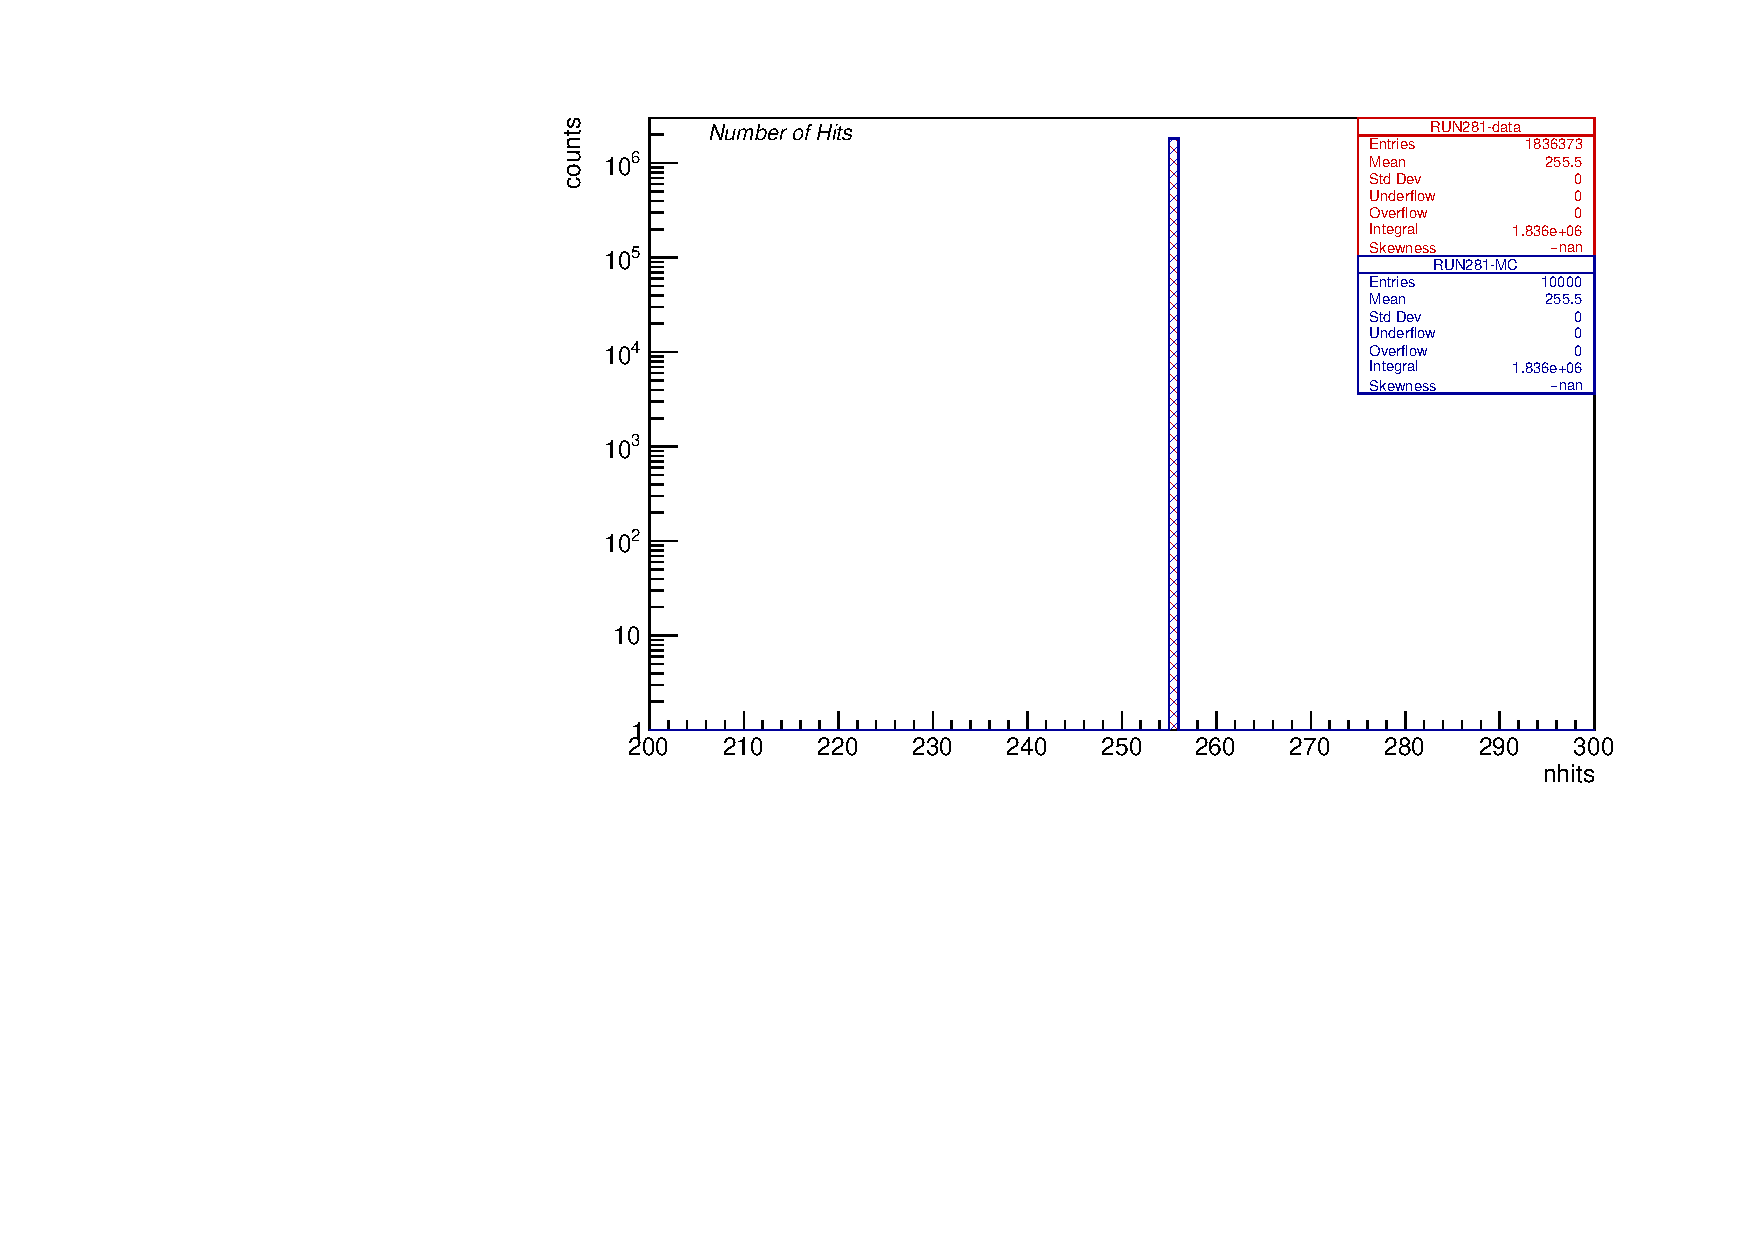
\includegraphics[width =0.7\textwidth]{figures/pdf/figure_00008_nhits_281.pdf}
\caption{
  The distribution of the total number of hits read out per event.
}
\label{fig:3}
\end{figure}
\subsection{The ``regular'' mode }
In the ``regular'' configuration, which will be referred to as RUN105038, the event window size is 25 $\mu$s
and the pulser rate is 60 kHz.

\subsubsection{Time distribution and occupancy}

Similar to Section \ref{over}, Figure \ref{fig:4} shows the distributions
of the number of hits in two channels, one from the 
FPGA-1 and another one, from the FPGA-2. 
In this readout configuration, the expected number of pulses in a given channel
within the event window is one or two, and the total number of pulses is always below 255.

\begin{figure}[!h]
  \begin{subfigure}[b]{\textwidth}
      \centering
      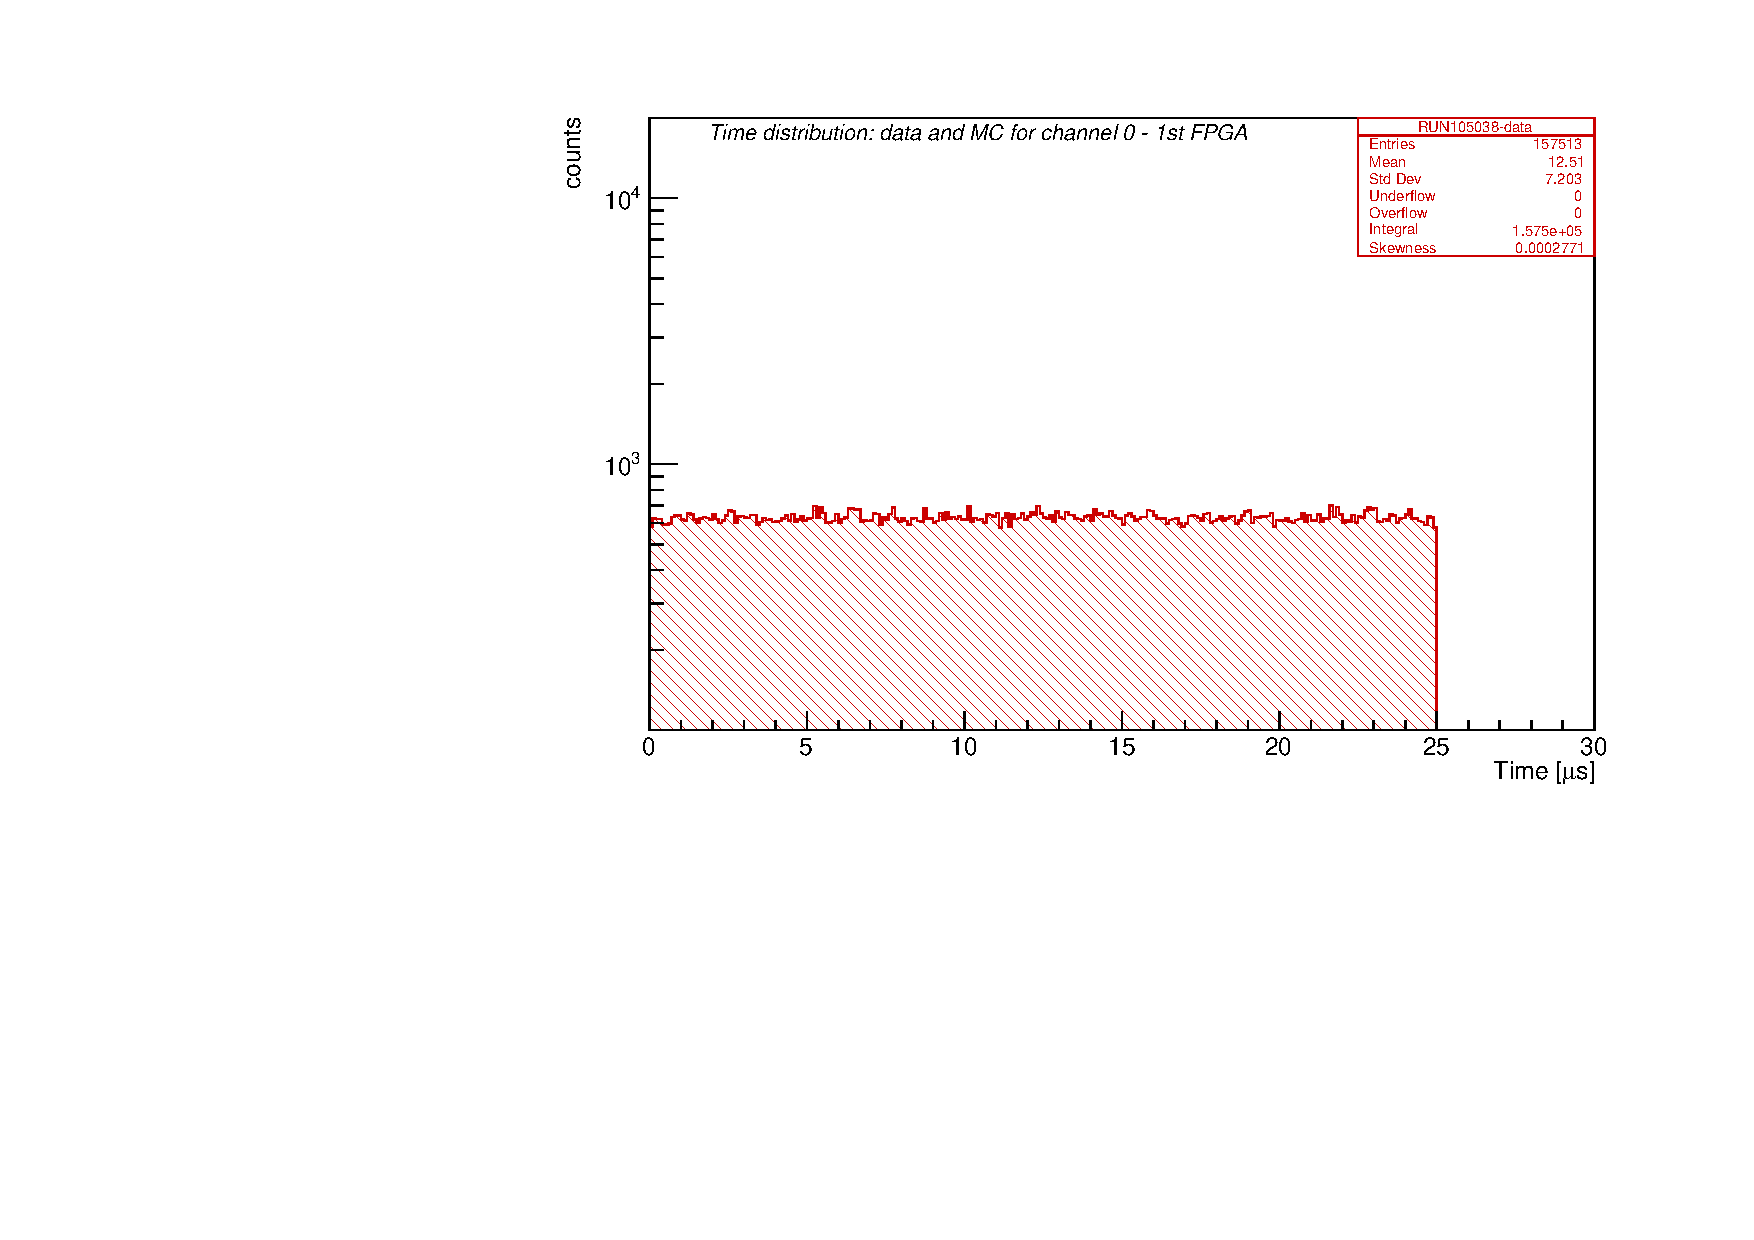
\includegraphics[width=0.7\textwidth]{figures/pdf/figure_00001_timedistr_roc_simulation_10538.pdf}
      \label{fig:ttt1}
  \end{subfigure}
\\
  \begin{subfigure}[b]{\textwidth}
      \centering
      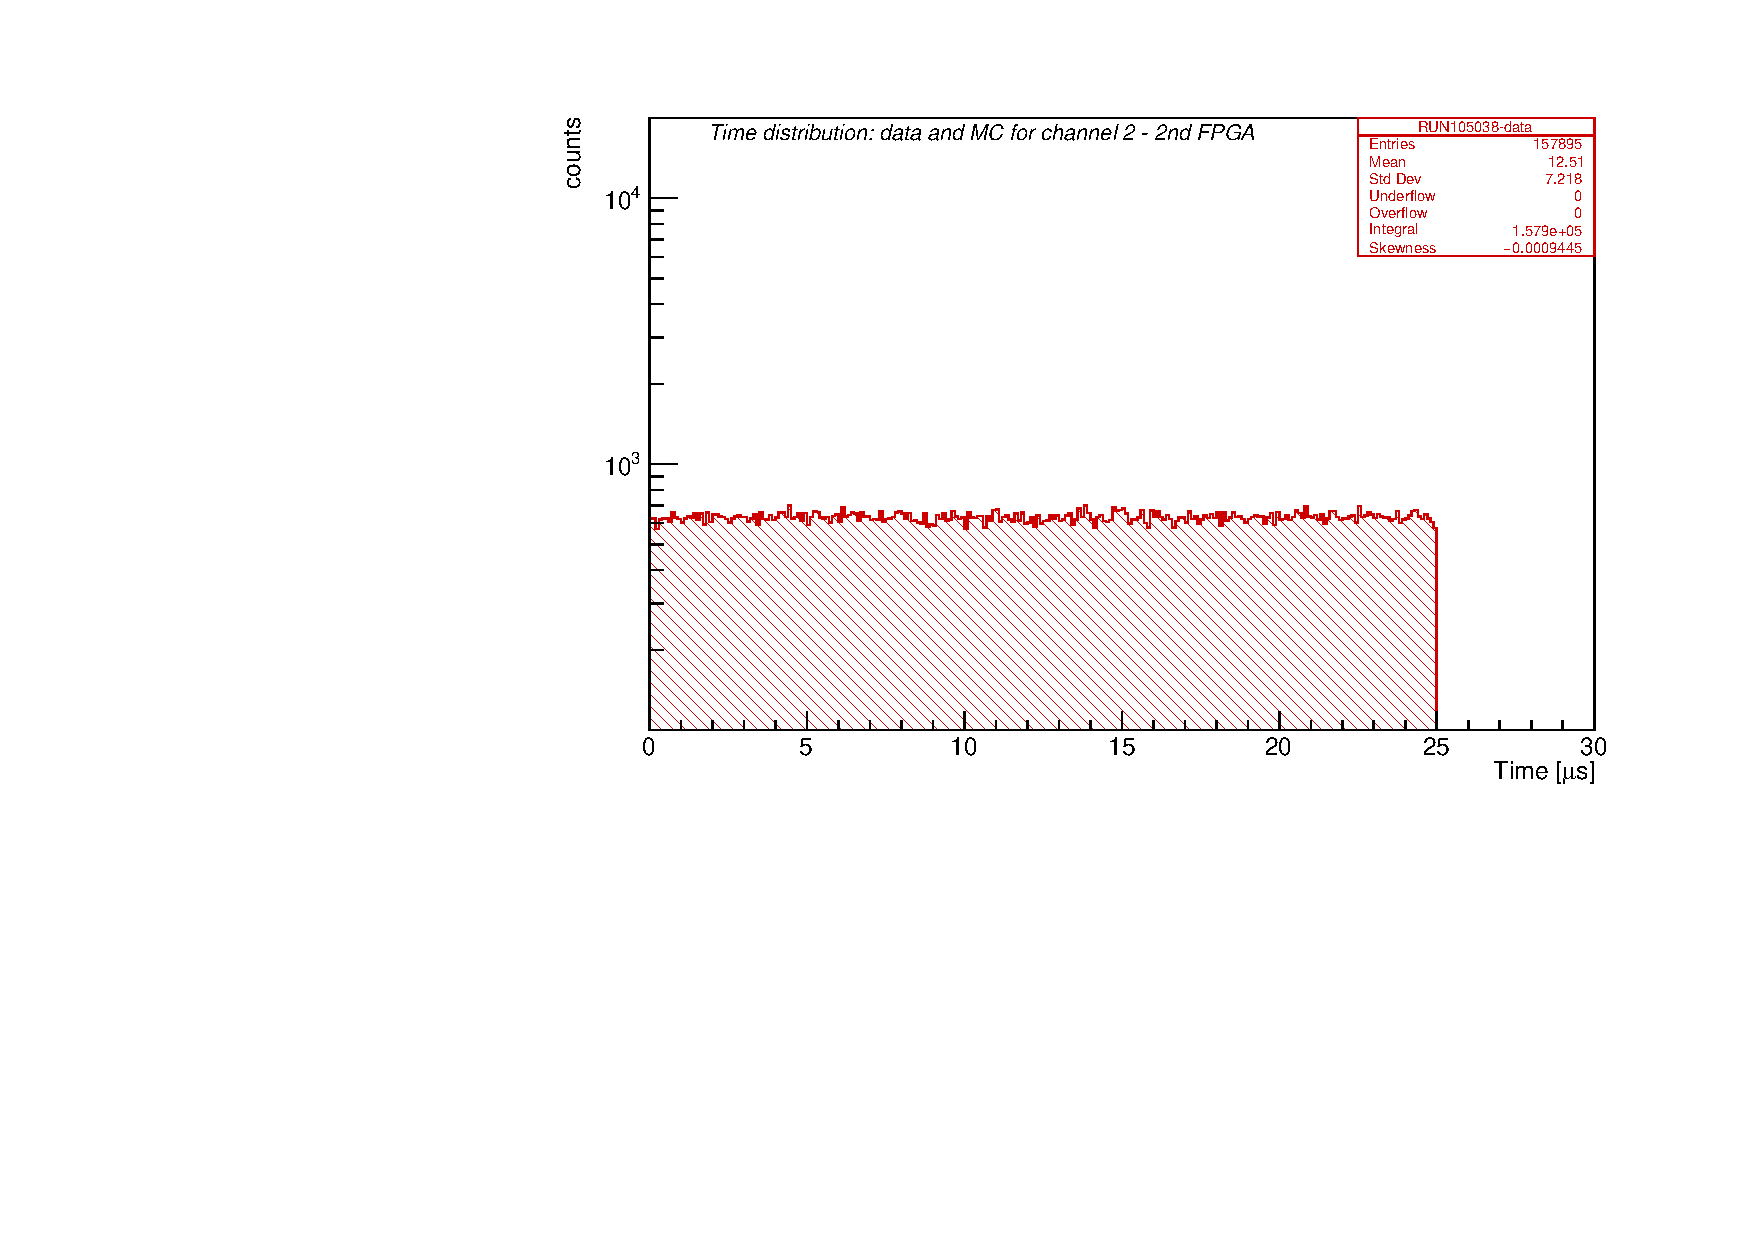
\includegraphics[width=0.7\textwidth]{figures/pdf/figure_00012_timedistr_roc_simulation_ch2_105038.pdf}
      \label{fig:ttt2}
  \end{subfigure}
     \caption{(Top): the hit time distribution for this in channel 2, the FPGA-2. 
     (Bottom): the hit time distribution for hits in channel 0, the FPGA-1.}
     \label{fig:4}
\end{figure}

In this mode, the readout of a given channel is not affected by the readout of previous
channels and the ``occupancy'' distributions shown in Figure \ref{fig:5} are, as expected, uniform.
\begin{figure}[!h]
\centering
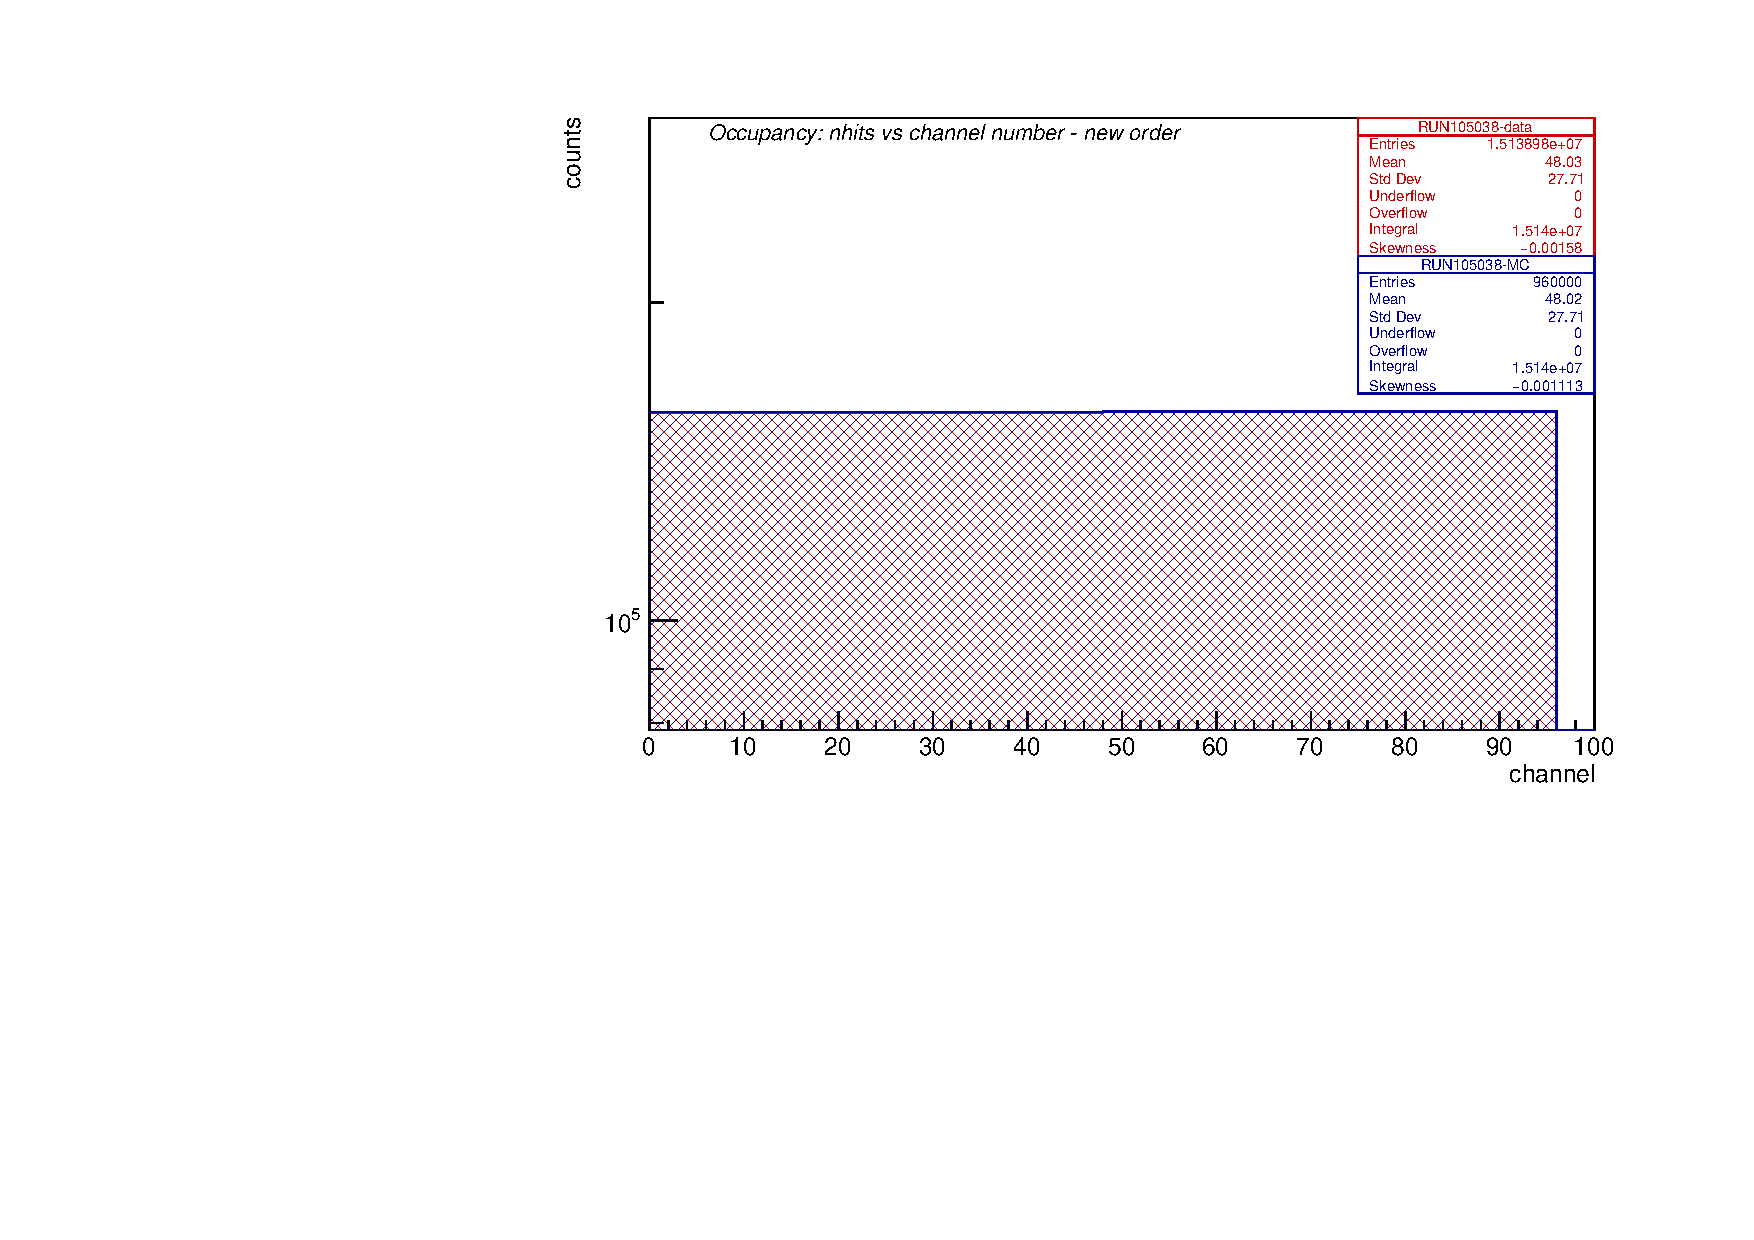
\includegraphics[width =0.7\textwidth]{figures/pdf/figure_00002_nhitsvschannel_roc_simulation_2.pdf}
\caption{Occupancy: the number of hits versus the channel number for RUN105038.}
\label{fig:5}
\end{figure}


Figure \ref{fig:67} shows the distribution of the number of hits in the channel 0 (FPGA-1).
\begin{figure}[!h]
\centering
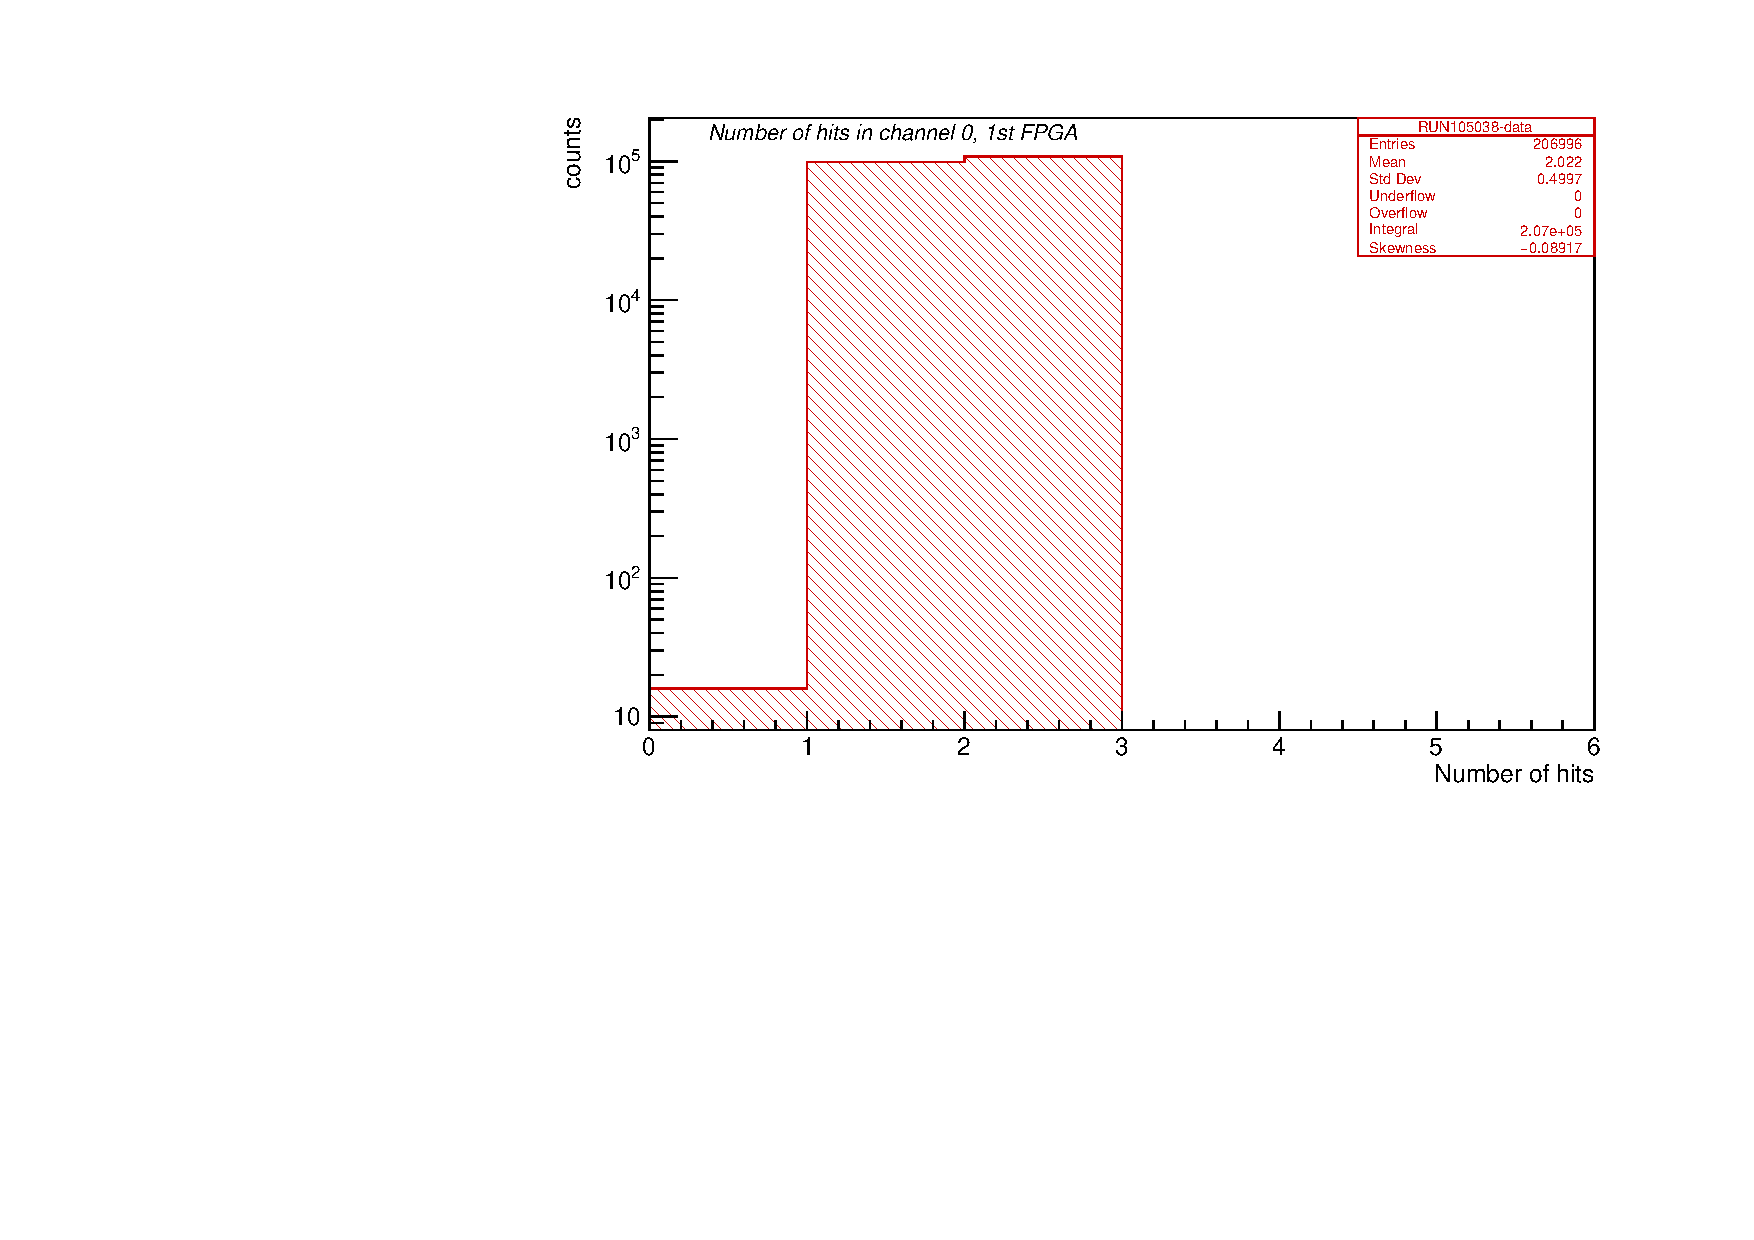
\includegraphics[width =0.7\textwidth]{figures/pdf/figure_00067_nhits_ch00_run105038.pdf}
\caption{
  The distribution of the number of hits in channel 0, FPGA-1, for RUN105038.
  Entries in the $n$(hits)=0 bin are due to the readout errors.
}
\label{fig:67}
\end{figure}

%%%%%%%%%%%%%%%%%%%%%%%%%%%%%%%%%%%%%%%%%%%%%%%%%%%%%%%%%%%%%%%%%%%%%%%%%%%%%%
\subsubsection{Number of hits}
Compared to RUN281, the event window in RUN105038 was twice shorter
and the ROC readout buffer wasn't getting filled up.
The total number of hits within the event window depends on the relative offset
of the event window with respect to the FPGA pulsers, and varies from
144 to 192, as shown in Figure \ref{fig:6}.

\begin{figure}[!h]
\centering
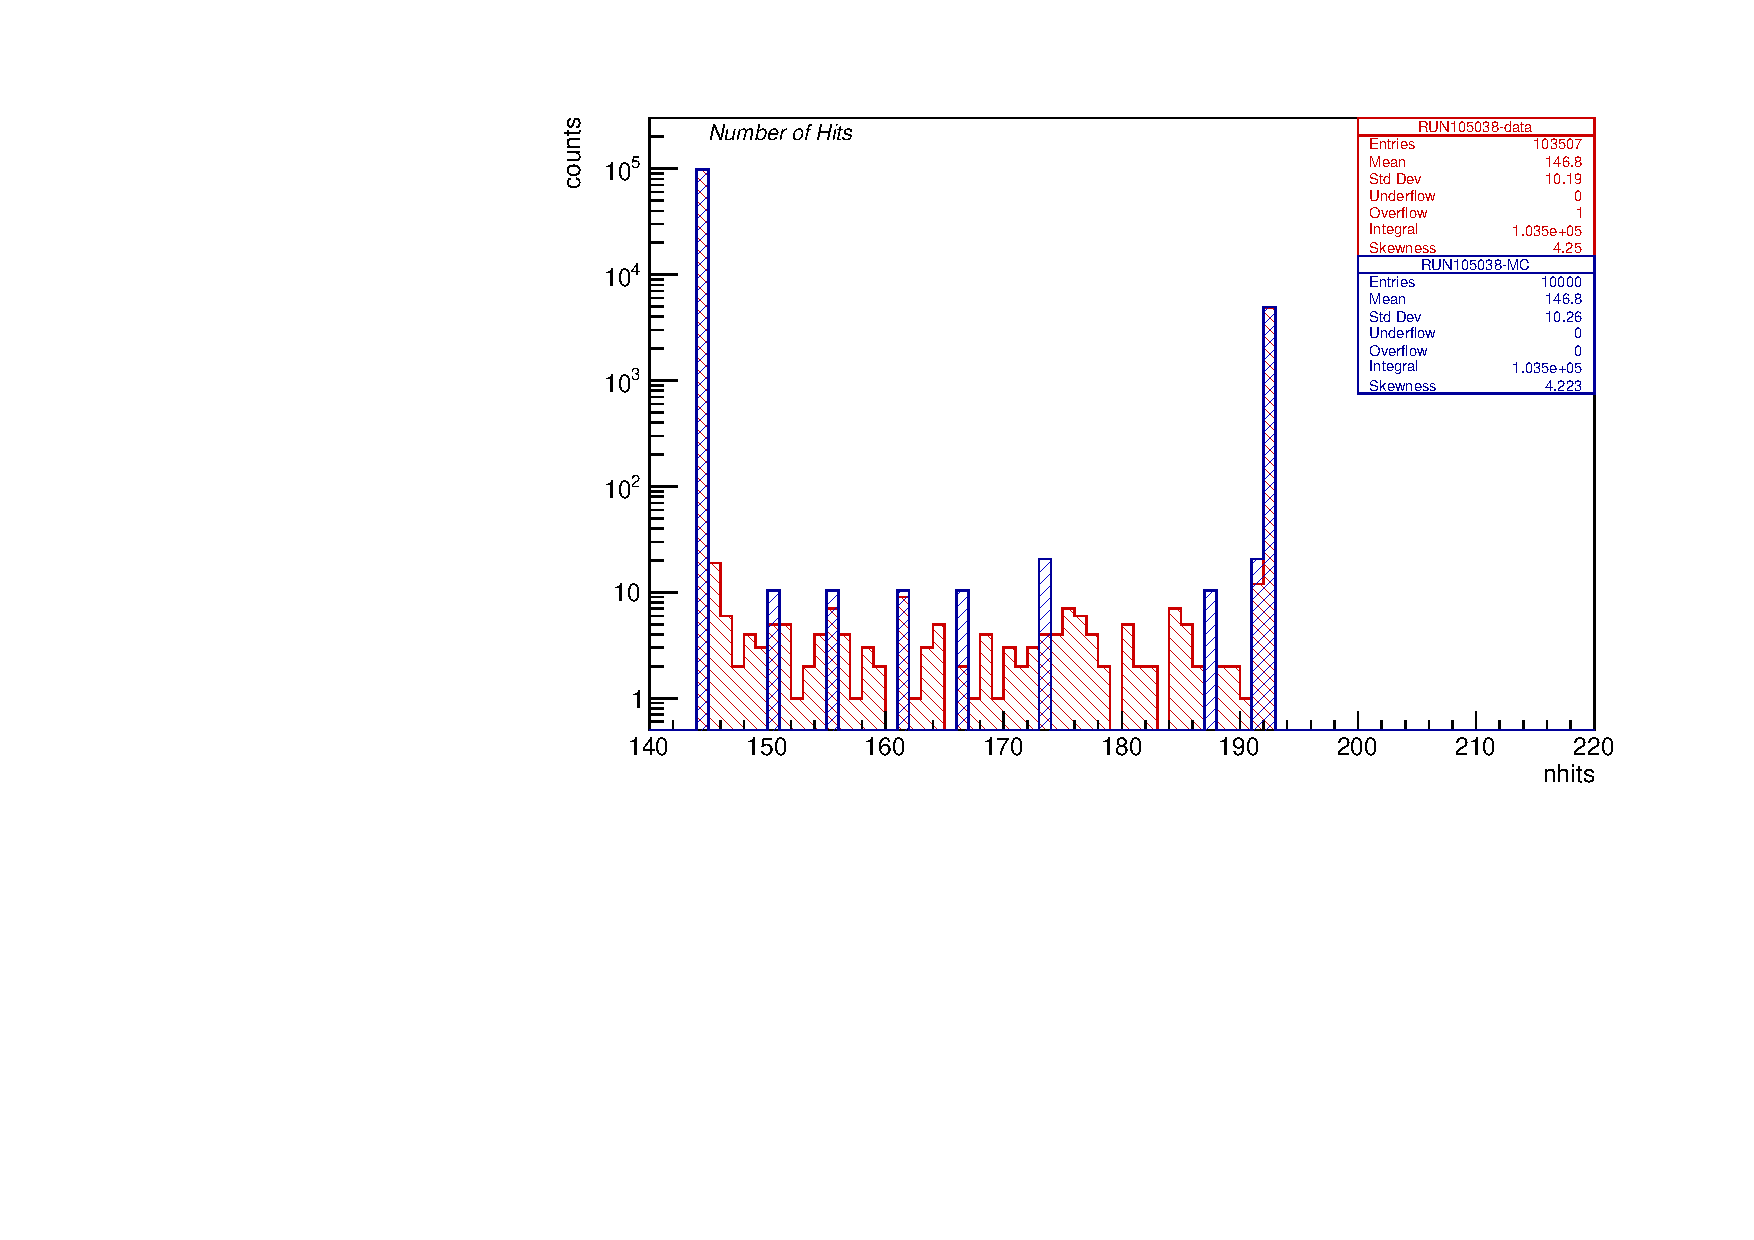
\includegraphics[width =0.7\textwidth]{figures/pdf/figure_00009_nhits_105038.pdf}
\caption{
  The distribution of the total number of hits per event in ``non-saturated'' mode.
}
\label{fig:6}
\end{figure}
\section{Primitive Data Quality Monitoring}\label{dqm}
The correct behaviour of the preamps was evaluated through the preamp charge injection test. Real-time monitoring and diagnostics were implemented.
The monitoring involves the creation of real-time histograms, which can easily assess 
the signal uniformity between channels within a single ROC, across multiple ROCs and among events.
The diagnostics involves the identification of error bits, such as the presence of an 
invalid channel ID, more hits than the maximum allowed in a given channel and an undefined link ID between ROCs.

\subsection{Number of hits versus channel ID}\label{nhitvschid}
The pulser implemented in the DRACs, as described in Section \ref{des}, was sending pulses to the preamps. 
The first aspect to examine was the assessment of the correct number of hits relative to the channel ID.
The charge injection pulser frequency was 50 kHz, with an EW of 50 $\mu$s. As previously explained, 
the number of pulses could vary (3 or 4 hits). This approach allowed us to determine if a channel was dead (0 hits), 
if there were more hits than expected in a given channel and if there were any cross talks between channels. 
Cross talks refer to the undesired signal coupling between channels. 
Pulses were sent every 8 channels to assess their presence. To study all channel, multiple runs were required.
Figure \ref{fig:normalhits} shows a regular distribution of number of hits versus channel ID.
\begin{figure}[!h]
      \centering
      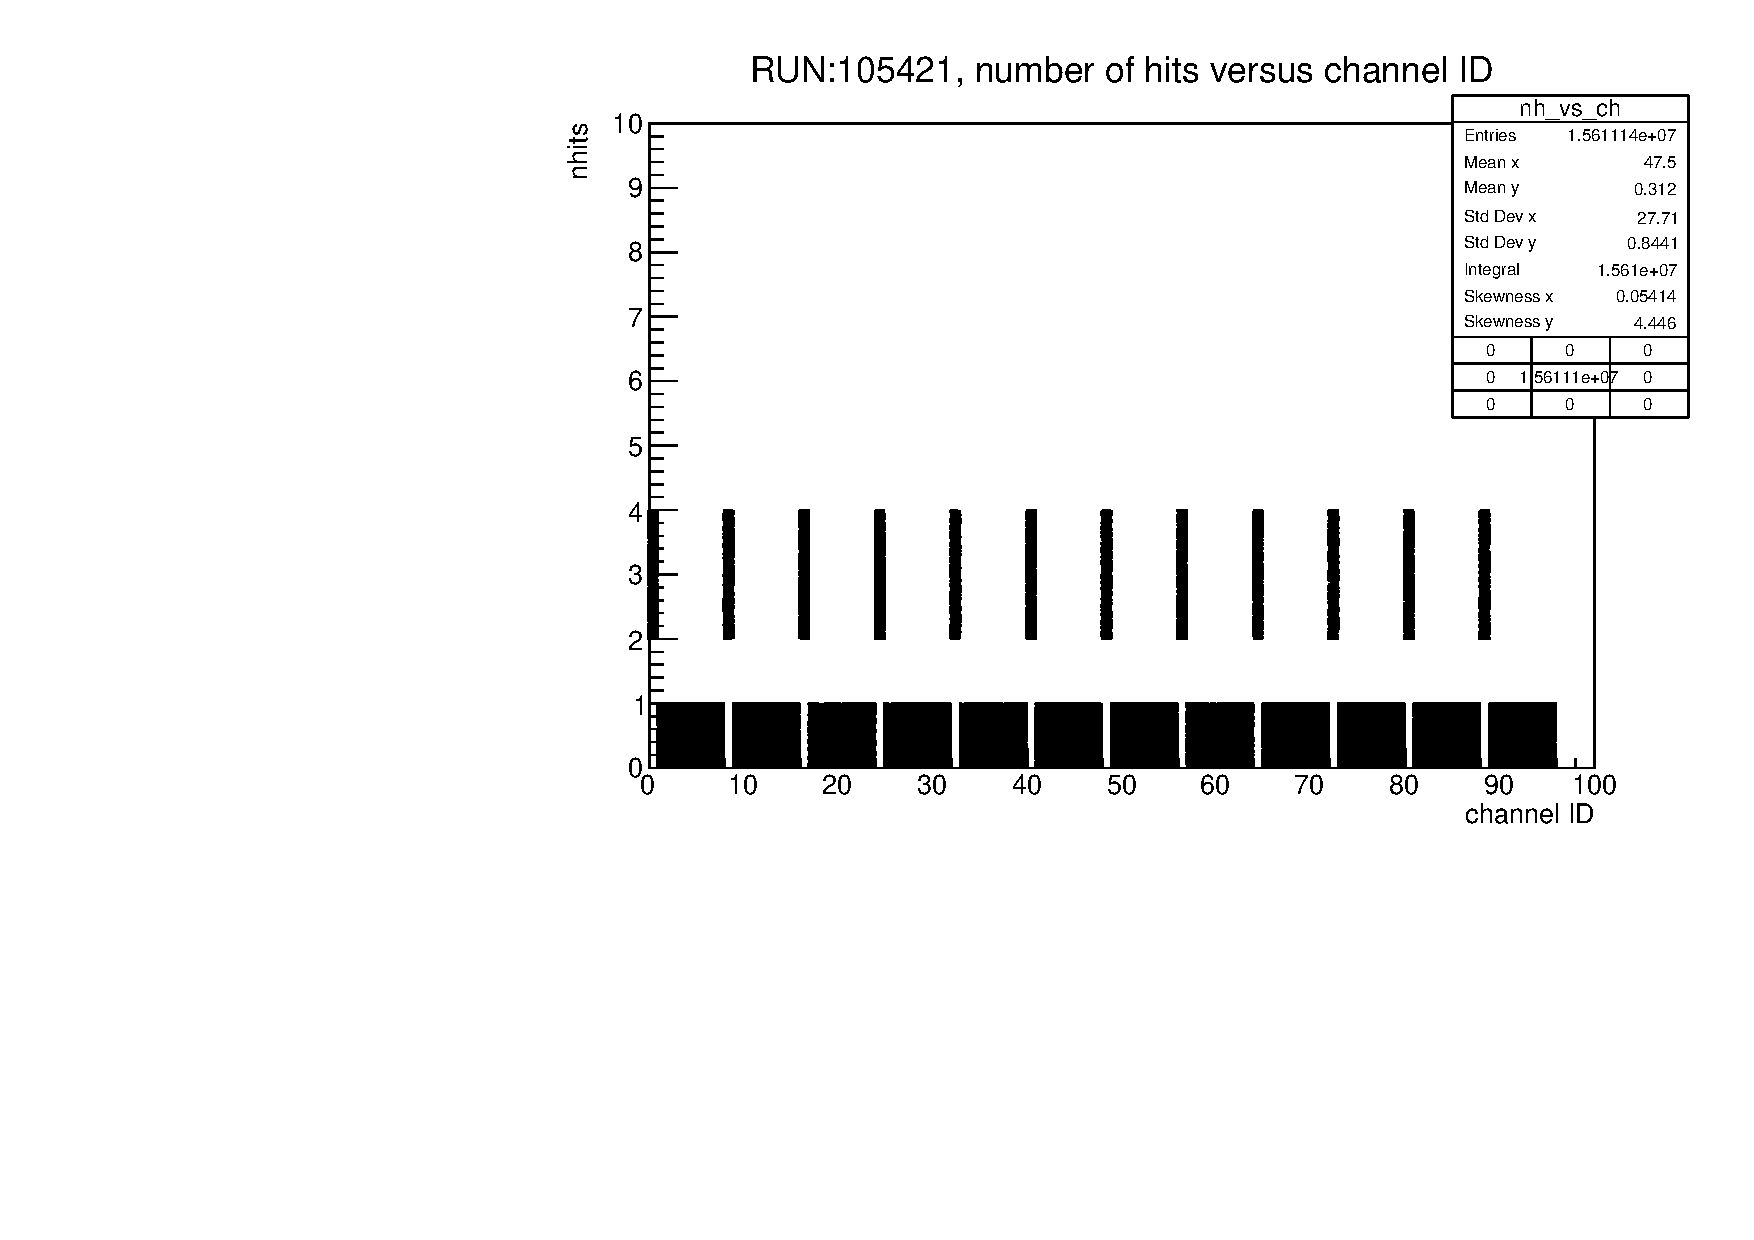
\includegraphics[width=0.65\textwidth]{figures/pdf/run105421_nh_vs_ch.pdf}
      \caption{Regular distribution of number of hits versus channel ID. The 0th channel is the first to be pulsed.
      As a consequence, the active channels are the 8th, 16th, 24th, 32nd, 40th, 48th, 56th, 64th, 72nd, 80th and 88th. The number of hits is 3 or 4 for all channels. 
      No cross talks were observed in any neighbour channel.}
     \label{fig:normalhits}
\end{figure}
Figure \ref{fig:dead} shows a run with a dead channel and a channel with more than four hits. 
In the case of the dead channel, the problematic preamp was replaced. In the second case, the 
$\Delta t$ distribution between hits was plotted, as shown in Figure \ref{fig:deltatnhits}.

\begin{figure}[!h]
  \centering
  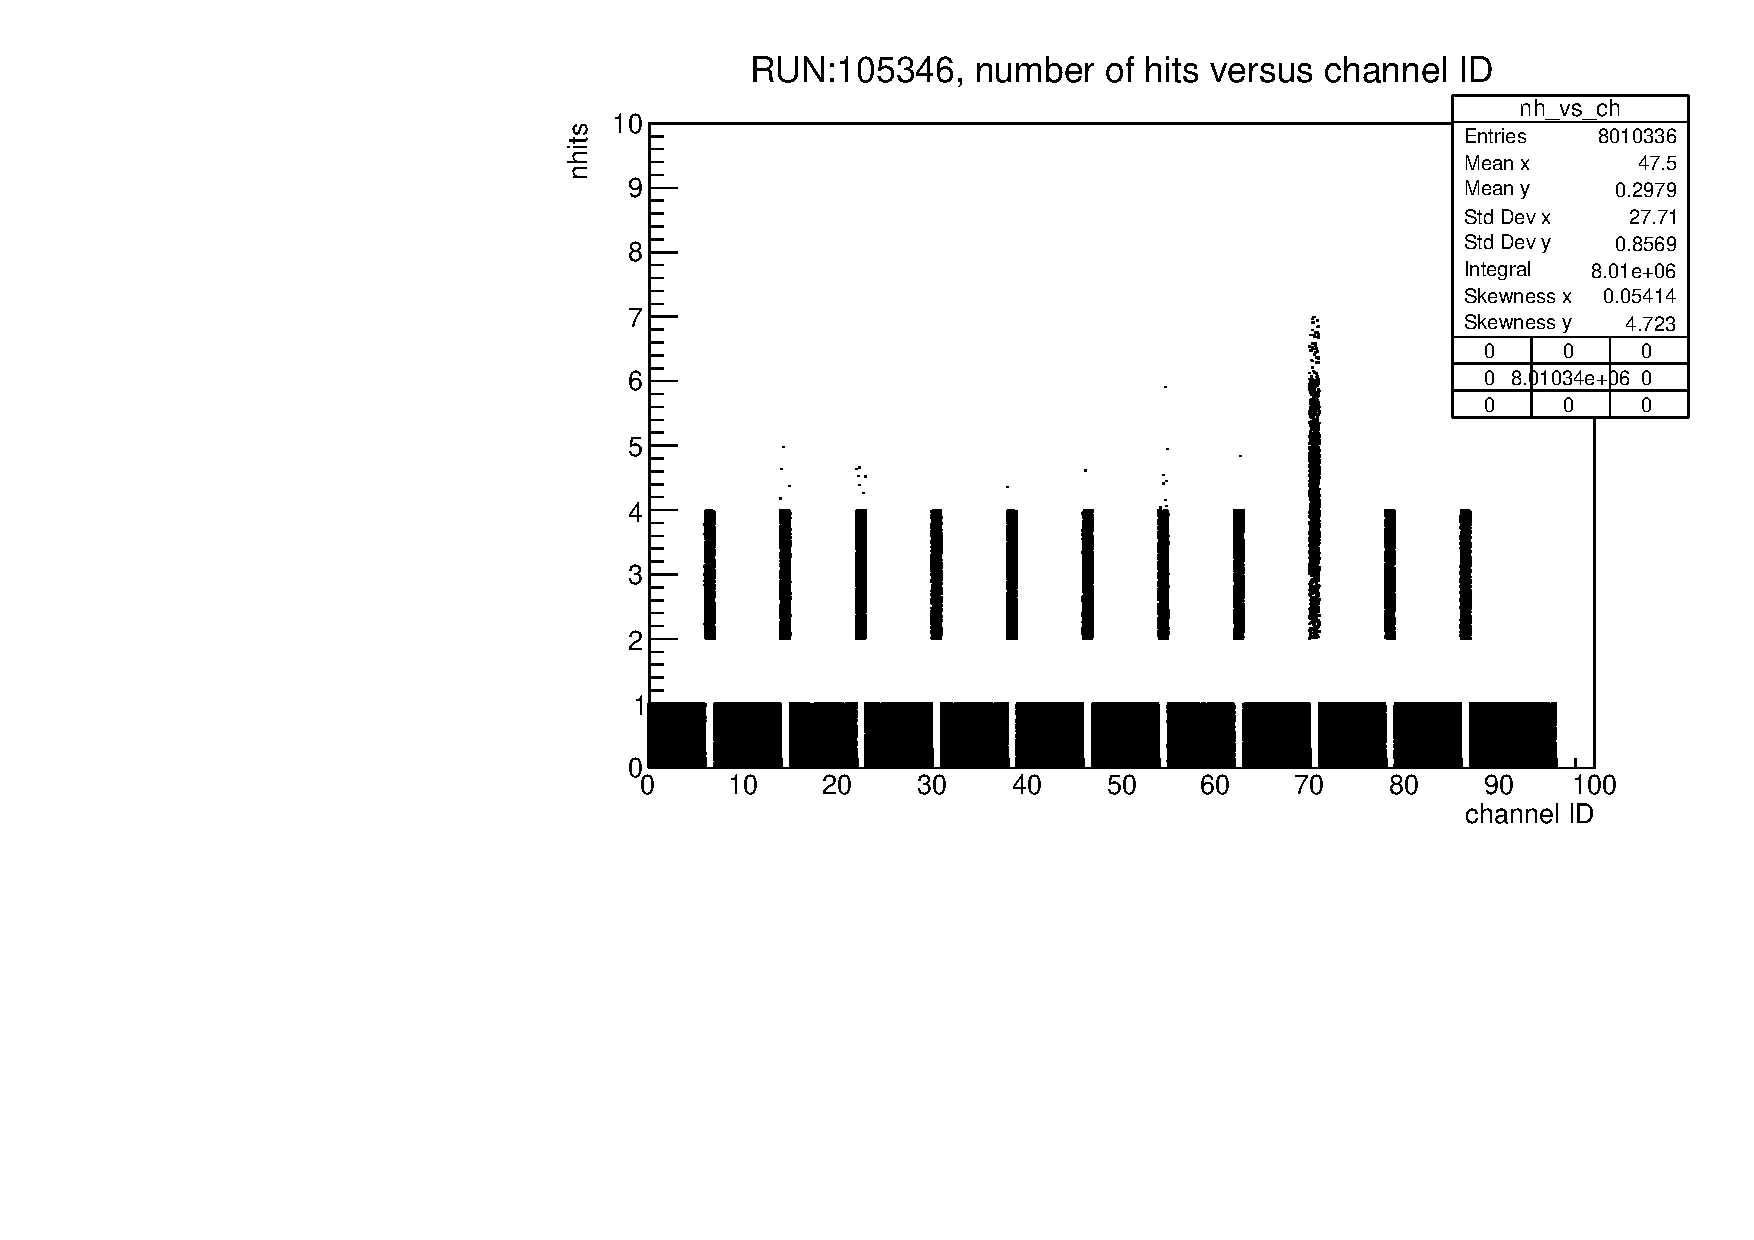
\includegraphics[width=0.65\textwidth]{figures/pdf/run105346_nh_vs_ch.pdf}
  \caption{Distribution of number of hits versus channel ID. The 6th channel is the first to be pulsed.
  As a consequence, the channels that should be active are the 14th, 22nd, 30th, 38th, 46th, 54th, 62nd, 70th, 78th, 86th and 94th. 
  The 94th channel is not responding. In this case, the preamp was substituted.
  The number of hits is not the same for all channels. The 14th, 22nd, 38th, 46th, 54th, 62nd, 70th channels have more hit than expected.
  To address this issue, the distribution of $\Delta t$ between hits of one of this channels is reported in Figure \ref{fig:deltatnhits}.
  No cross talks were observed in any neighbour channel.}
 \label{fig:dead}
\end{figure}


\begin{figure}[!h]
  \centering
  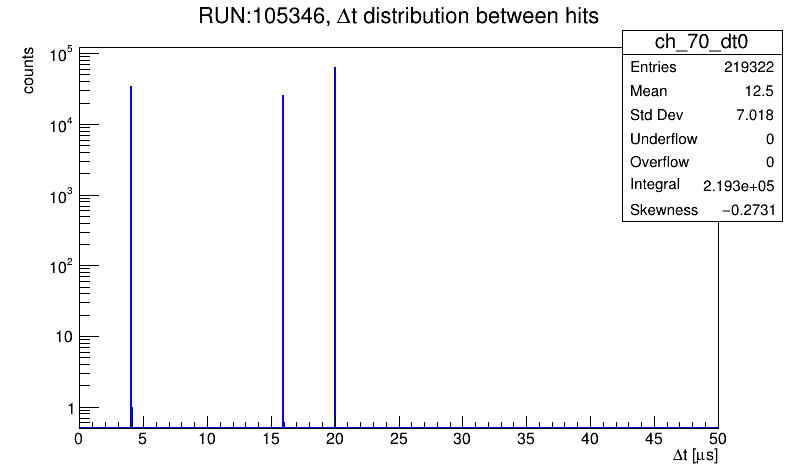
\includegraphics[width=0.65\textwidth]{figures/png/deltathits.png}
  \caption{$\Delta t$ distribution between hits in the 70th channel. The $\Delta t$ distribution between hits 
  should peak at 20 $\mu$s, as the pulser operates at a frequency of 50 kHz. However, peaks at approximately 
  16 $\mu$s and 4 $\mu$s are observed. All waveforms at around 4 $\mu$s are inverted compared to the regular ones. 
  The waveforms are shown in Section \ref{wf}, and the reason for this behaviour will be explained in the same section.}
 \label{fig:deltatnhits}
\end{figure}

One more important feature to be investigated is the presence of cross talks. Figure \ref{fig:cross} shows a run where cross talk is detected.
This phenomenon occurred only when the first pulsed channel is odd. The cross talk is asymmetric (3$\rightarrow$5 is observed, 
but no 3$\rightarrow$1) and only in odd channels.
As mentioned in chapter \ref{tracker}, the preamps are mounted vertically and one preamp refers to two channels: odd channels are the ones on the board, 
while even ones are on the top. For this reason, the cross talk appears to be between channels plced on the board. 
Additionally, it seems to occur only in the first 20 channel IDs.
The space between the first preamps is narrower compared to the others, as shown in Figure \ref{fig:spacepreamps}. 
\begin{figure}[!h]
  \centering
  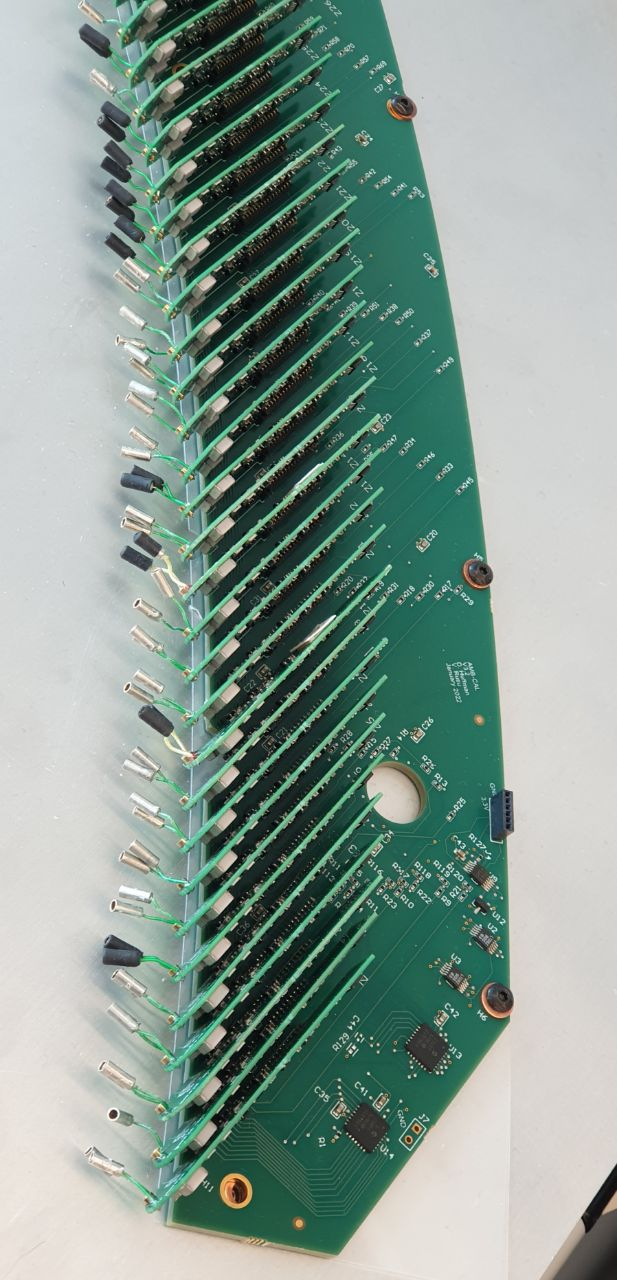
\includegraphics[angle=90,width=\textwidth]{figures/jpg/photo_6028424923279639562_y.jpg}
  \caption{The spacing between preamps on the board. The first channels correspond to the preamps on the right side of the picture.}
 \label{fig:spacepreamps}
\end{figure}
This seems to be the reason why it happens only in the first channels. This behaviour was reported to the tracker panel experts, and they are still working on it.
\begin{figure}[!h]
  \centering
  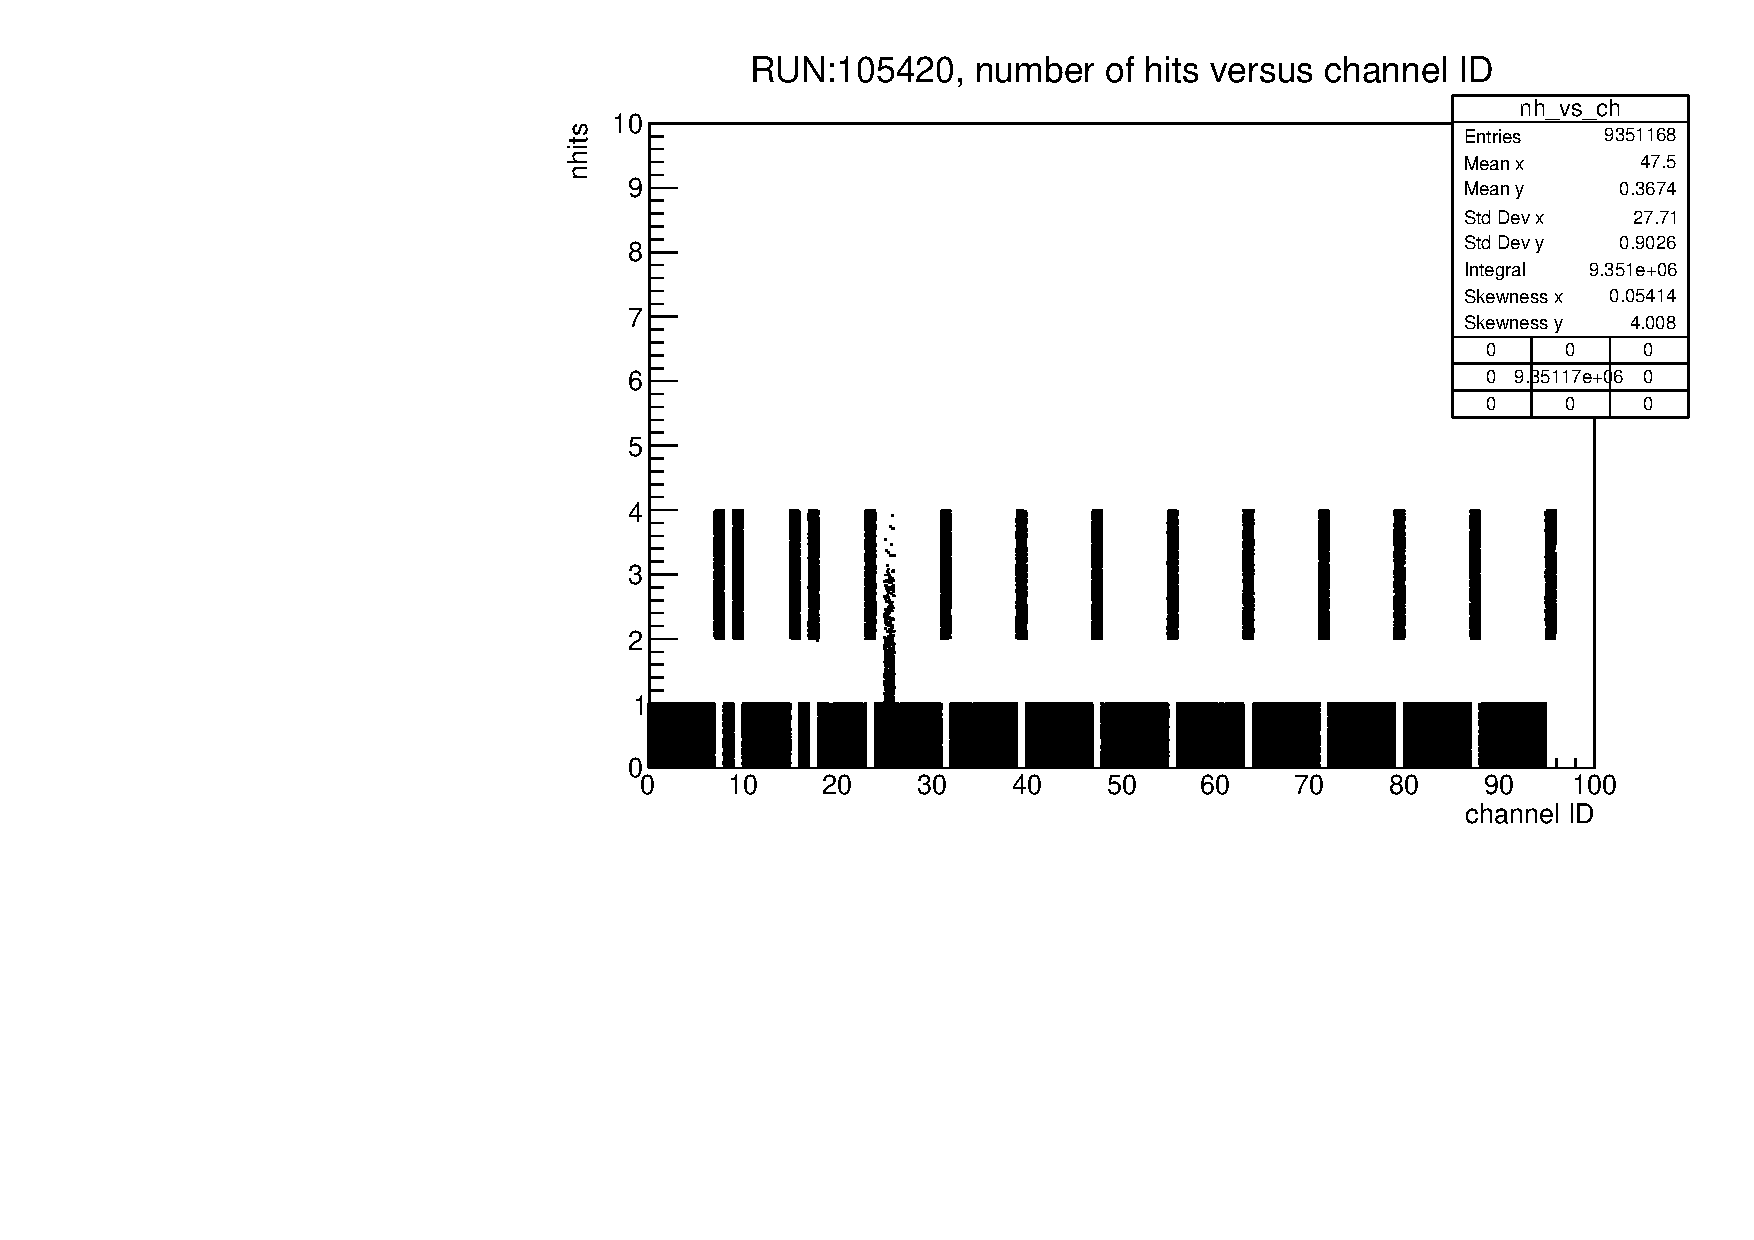
\includegraphics[width=0.65\textwidth]{figures/pdf/run105420_nh_vs_ch.pdf}
  \caption{Distribution of the number of hits versus channel ID. The 7th channel is the first to be pulsed. 
  As a consequence, the only channels that should be active are the 15th, 23rd, 31st, 39th, 47th, 55th, 63rd, 71st, 79th, 87th and 95th. 
  Channels 9th, 17th and 25th were also observed to be active, indicating cross talks.}
 \label{fig:cross}
\end{figure}
\subsection{Waveforms analysis}\label{wf}
The shape of charge injection waveforms has been reconstructed. As mentioned in Section \ref{DRAC}, 
the ADC has a sampling frequency of 40 MHz, resulting in a waveform bin width of 25 ns. 
The maximum number of samples is 30. To reconstruct the waveform, the baseline, as will be 
explained in more detail in Section \ref{basel}, is already subtracted.
Figure \ref{fig:normalwf} shows a regular reconstructed waveform for RUN105421.
\begin{figure}[!h]
  \centering
  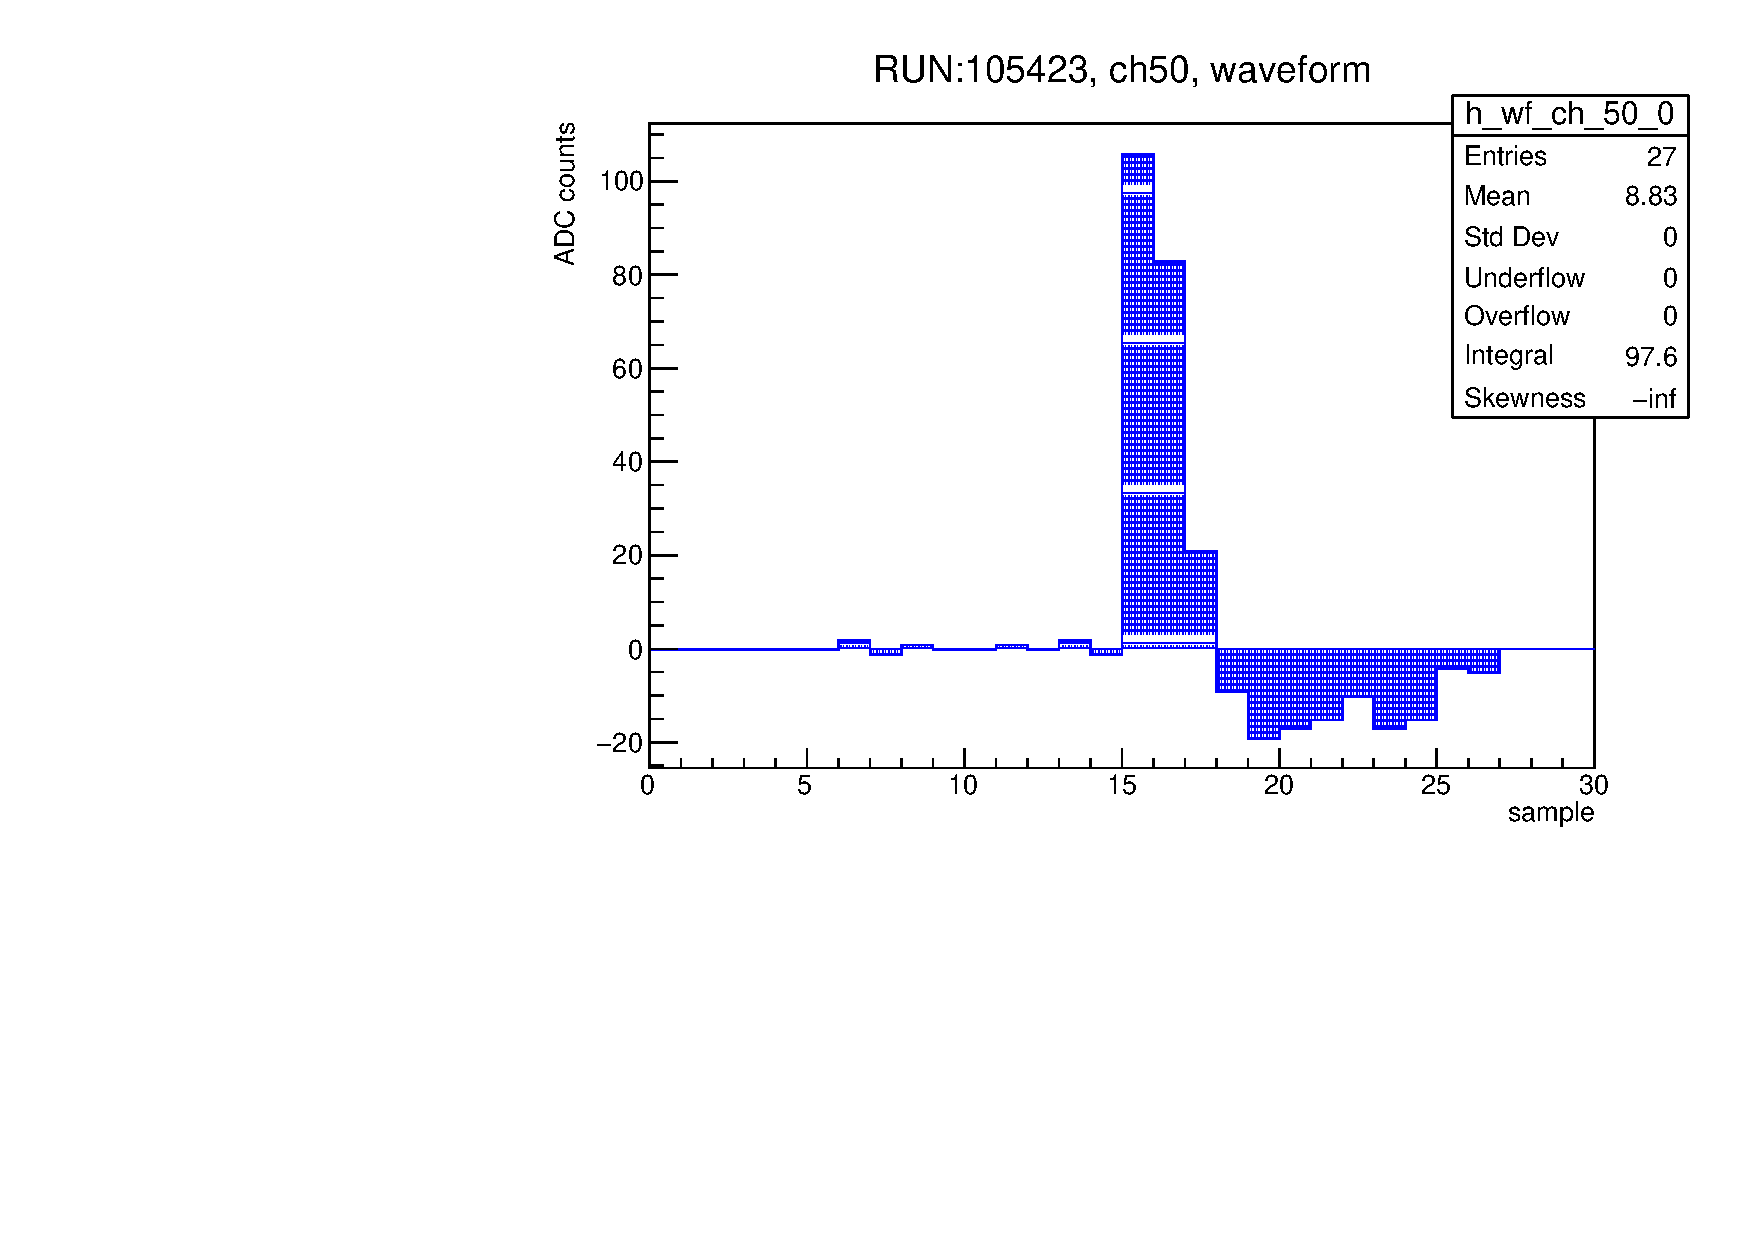
\includegraphics[width=0.65\textwidth]{figures/pdf/wf_ch50_0.pdf}
  \caption{Regular waveform of the 50th channel.}
 \label{fig:normalwf}
\end{figure}

The waveforms' negative tail is caused by a differentiating circuit, which approximately shapes a signal pulse using an high pass filter. 
At high count rates, it is possible for another pulse to arrive before the previous pulse has returned to zero, causing it to overlap with the undershoot of the initial pulse. 
This reduces the apparent amplitude of the second pulse, leading to unwanted broadening of peaks in the energy spectrum. 
The rapid leading edge of the pulse remains unchanged due to the differentiator's time constant, which is not significantly 
shorter than the pulse's rise time. 



As discussed in Section \ref{nhitvschid}, a higher number of hits in some channels is observed, 
leading to a different $\Delta t$ distribution between hits than expected. 
While the $\Delta t$ peak was expected at 20 $\mu$s, in some channels two additional peaks were identified: 
one at 16 $\mu$s and another at 4 $\mu$s. The 4 $\mu$s peak is characterized by inverted waveforms, as shown in Figure \ref{fig:inverted}. 
The 16 $\mu$s peak is characterized by regular waveforms, as the 20 $\mu$s peak.
It is reasonable to think that this phenomenon arises from the erroneous generation of 4 $\mu$s long pulses, 
triggering them on both the leading and trailing edges. In fact, the sum of 4 $\mu$s and 16 $\mu$s is the inverse of the pulser frequency. 
One potential solution to address this issue could involve varying the pulse length. 
However, this approach was not pursued in this Thesis due to time constraints.
\begin{figure}[!h]
  \centering
  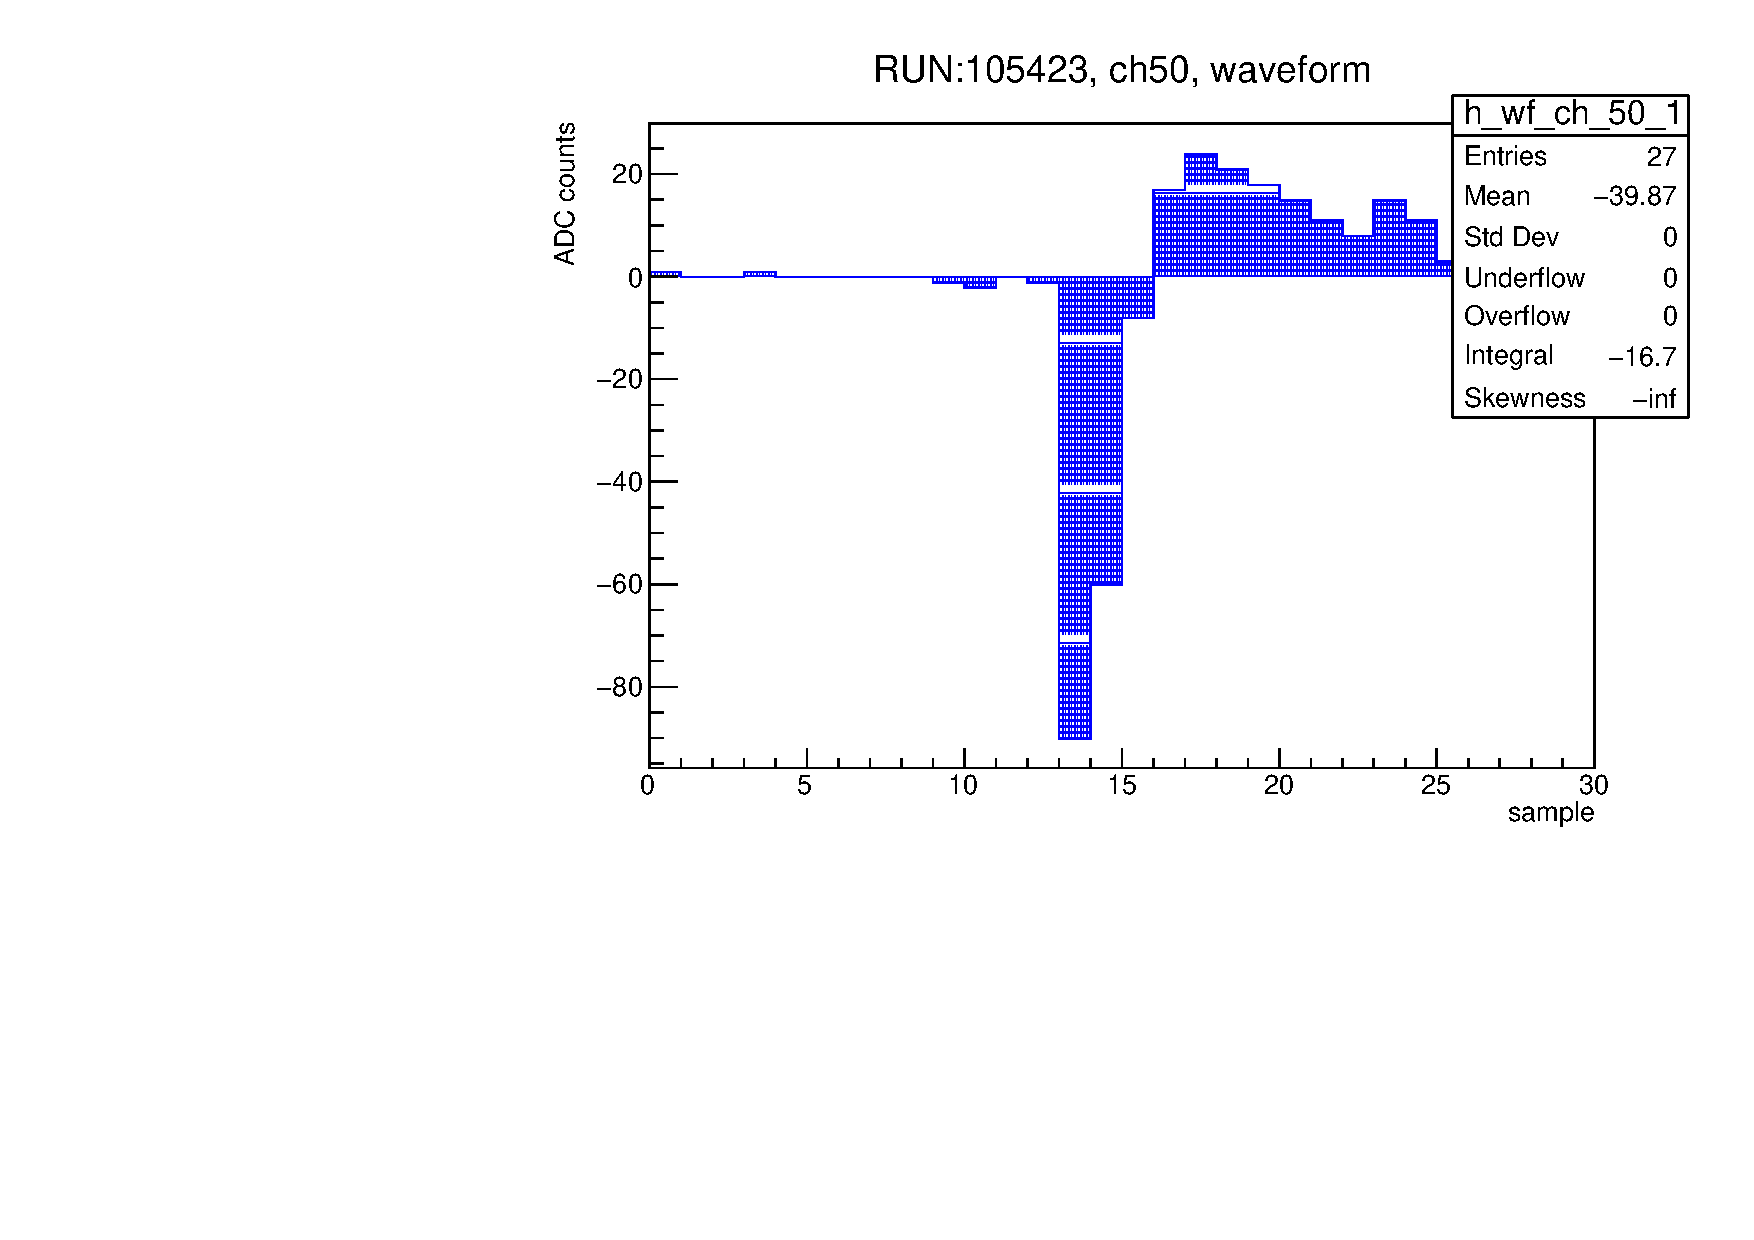
\includegraphics[width=0.65\textwidth]{figures/pdf/wf_ch50_1.pdf}
  \caption{Inverted waveform of the 50th channel.}
 \label{fig:inverted}
\end{figure}
\subsubsection{The waveform baseline}\label{basel}
The baseline can be estimated with the mean of the firsts 10 samples of the waveform. 
The pedestals for each channel vary according on the electrical component's tolerances on the board.
The pedestal stability is an indicator of the low noise of the electronic chain.
Figures \ref{fig:baseline1} and \ref{fig:baseline2} shows the baseline distribution for two different channels in RUN105421.
For both channels the pedestal is close to 210 ADC counts with a FWHM$=2 \sqrt{2 \text{ln}2}\sigma\sim$4.5 ADC counts.
  \begin{figure}[!h]
      \centering
      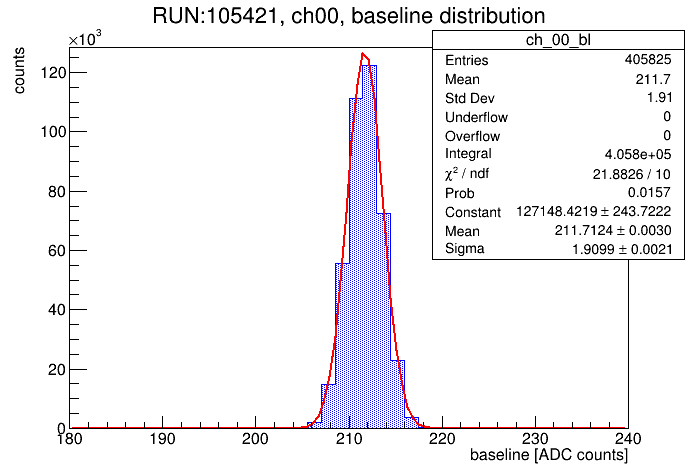
\includegraphics[width=0.65\textwidth]{figures/png/baseline_ch00.png}
      \caption{The fitted baseline distribution of channel 0.}
      \label{fig:baseline1}
  \end{figure}
  \begin{figure}[!h]
      \centering
      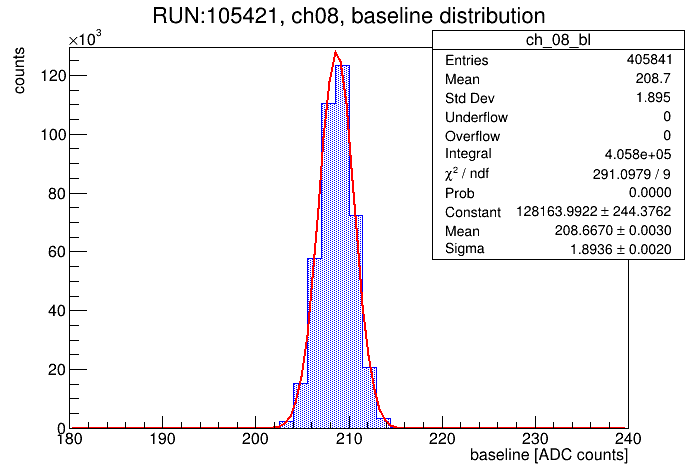
\includegraphics[width=0.65\textwidth]{figures/png/baseline_ch08.png}
      \caption{The fitted baseline distribution of channel 8.}
      \label{fig:baseline2}
\end{figure}

In some cases, a lower baseline value is observed. Examining the waveform, dips were identified with depths of 64, 128, or 192, 
suggesting the possibility of 6th and 7th bit errors in the ADC. Such waveform is shown in Figure \ref{fig:dips}. 
To address this issue, these waveforms were reconstructed by isolating the negative peaks and computing the mean of the remaining samples.
\begin{figure}[!h]
  \centering
  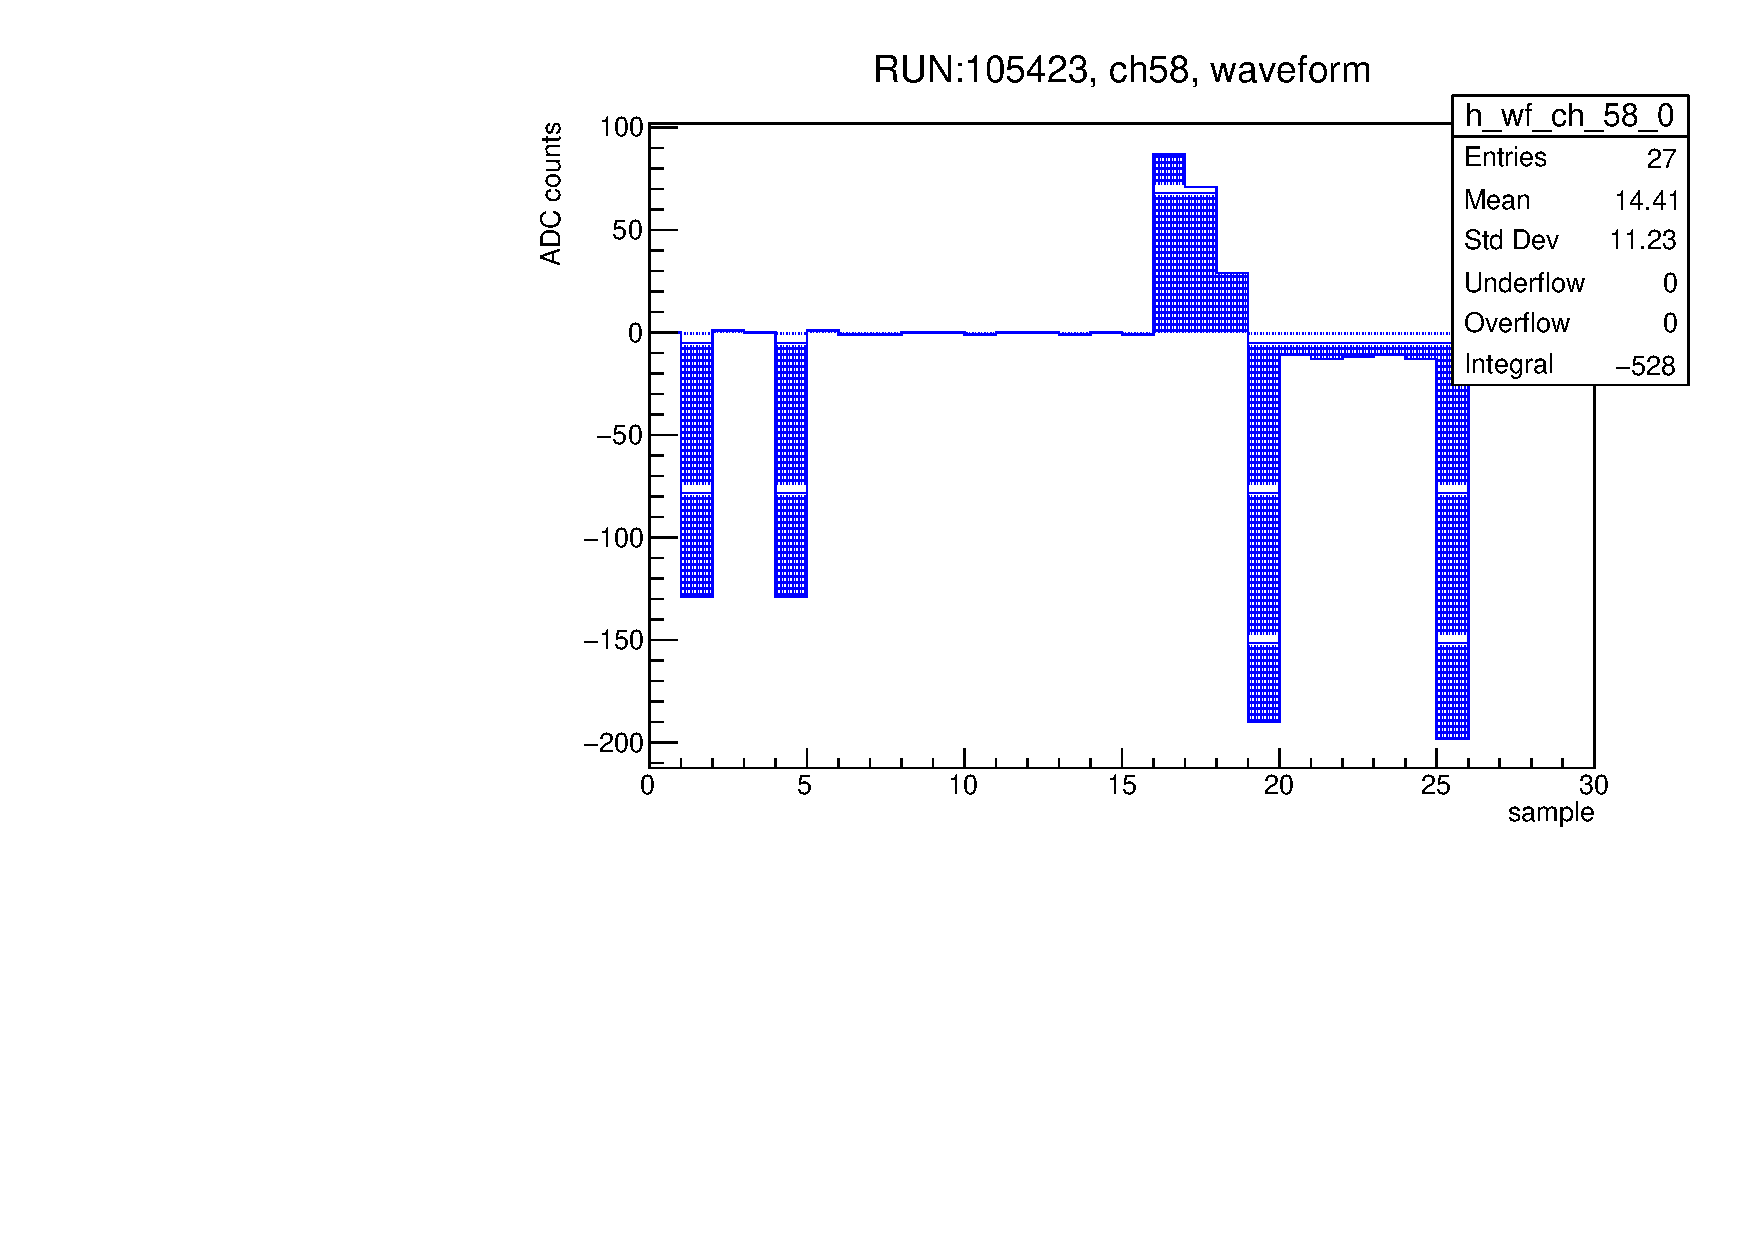
\includegraphics[width=0.65\textwidth]{figures/pdf/wf_ch58_1.pdf}
  \caption{Waveform of the 58th channel. Before subtracting the baseline from the ADC counts, the dips were identified. The depth of the dips is 128.}
 \label{fig:dips}
\end{figure}
\subsubsection{The waveform charge and pulse height}\label{threshold}
Using a constant threshold discriminator, the integral of the positive and negative parts of the waveform, 
the pulse height and the first sample were computed. The threshold was set to 5 ADC counts. 
The first sample is defined as the first one to be above the threshold, and the positive charge 
is the integral of the region above the threshold. The negative charge is the integral of the waveform's 
negative tail. The pulse height is the highest ADC count reached by the waveform. The distributions of 
charge, pulse height, first sample and negative charge are shown in Figures \ref{fig:ch1}, \ref{fig:ph2}, \ref{fig:fs2}, and \ref{fig:nch2}.

\begin{figure}[!h]
      \centering
      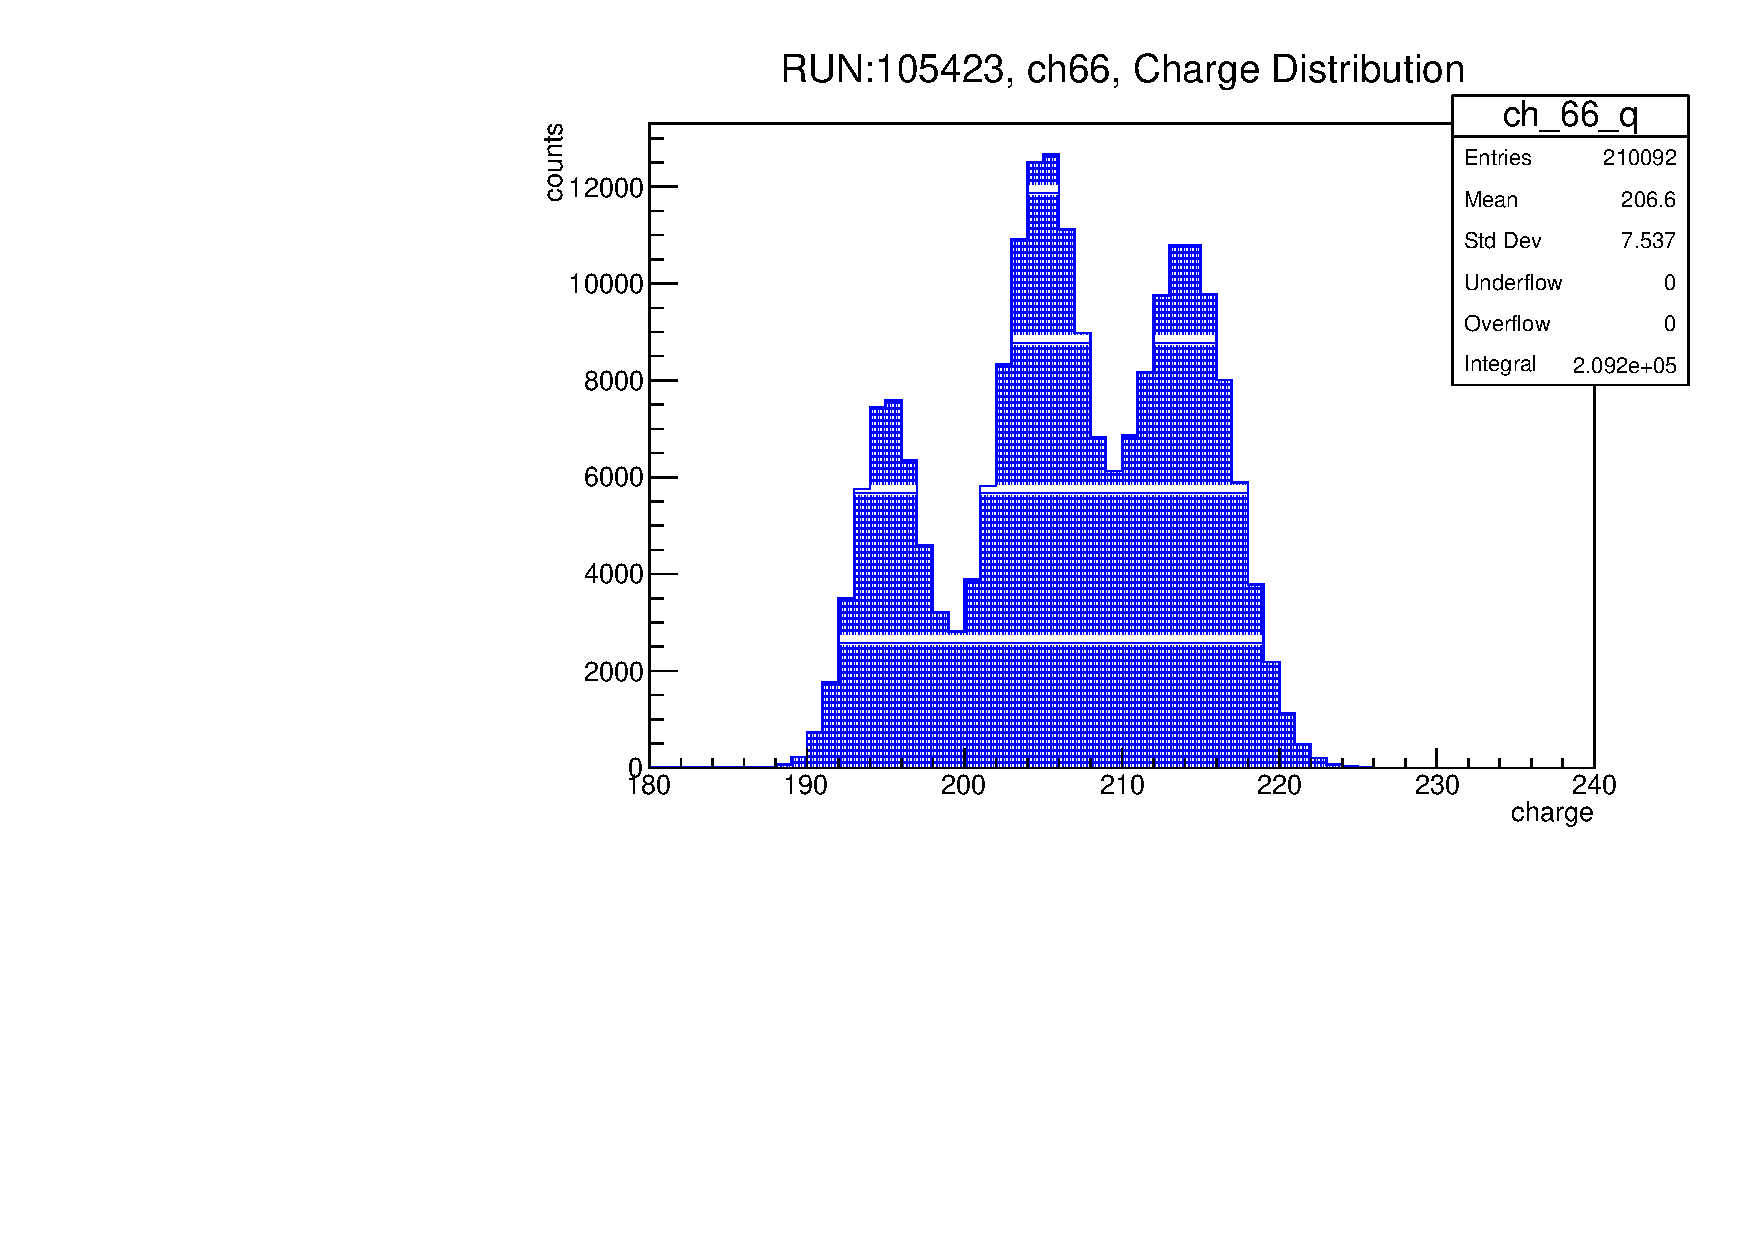
\includegraphics[width=0.65\textwidth]{figures/pdf/charge.pdf}
      \caption{Charge distribution of the waveforms in channel 66.}
      \label{fig:ch1}
  \end{figure}

\begin{figure}[!h]
  \centering
  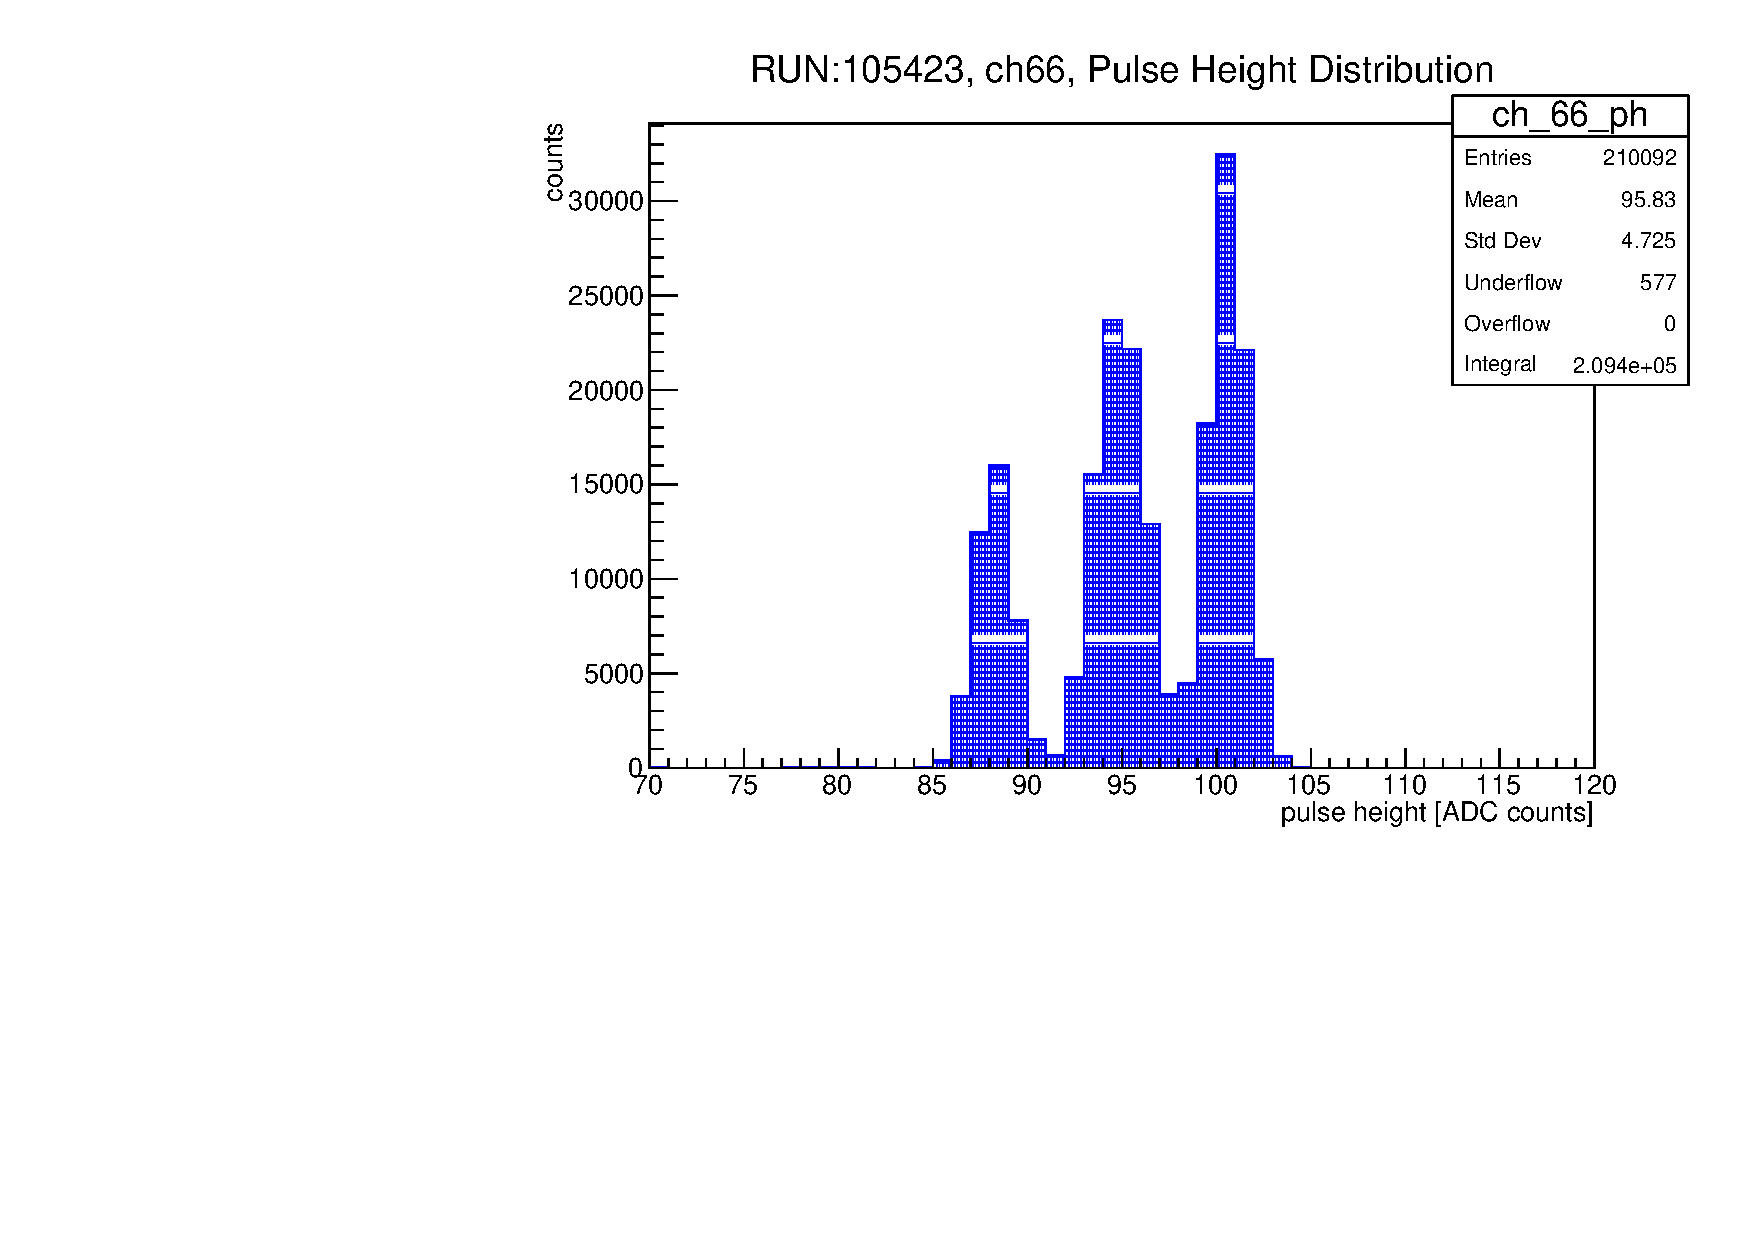
\includegraphics[width=0.65\textwidth]{figures/pdf/pulseheight.pdf}
  \caption{Pulse height distribution of the waveforms in channel 66.}
  \label{fig:ph2}
\end{figure}

\begin{figure}[!h]
  \centering
  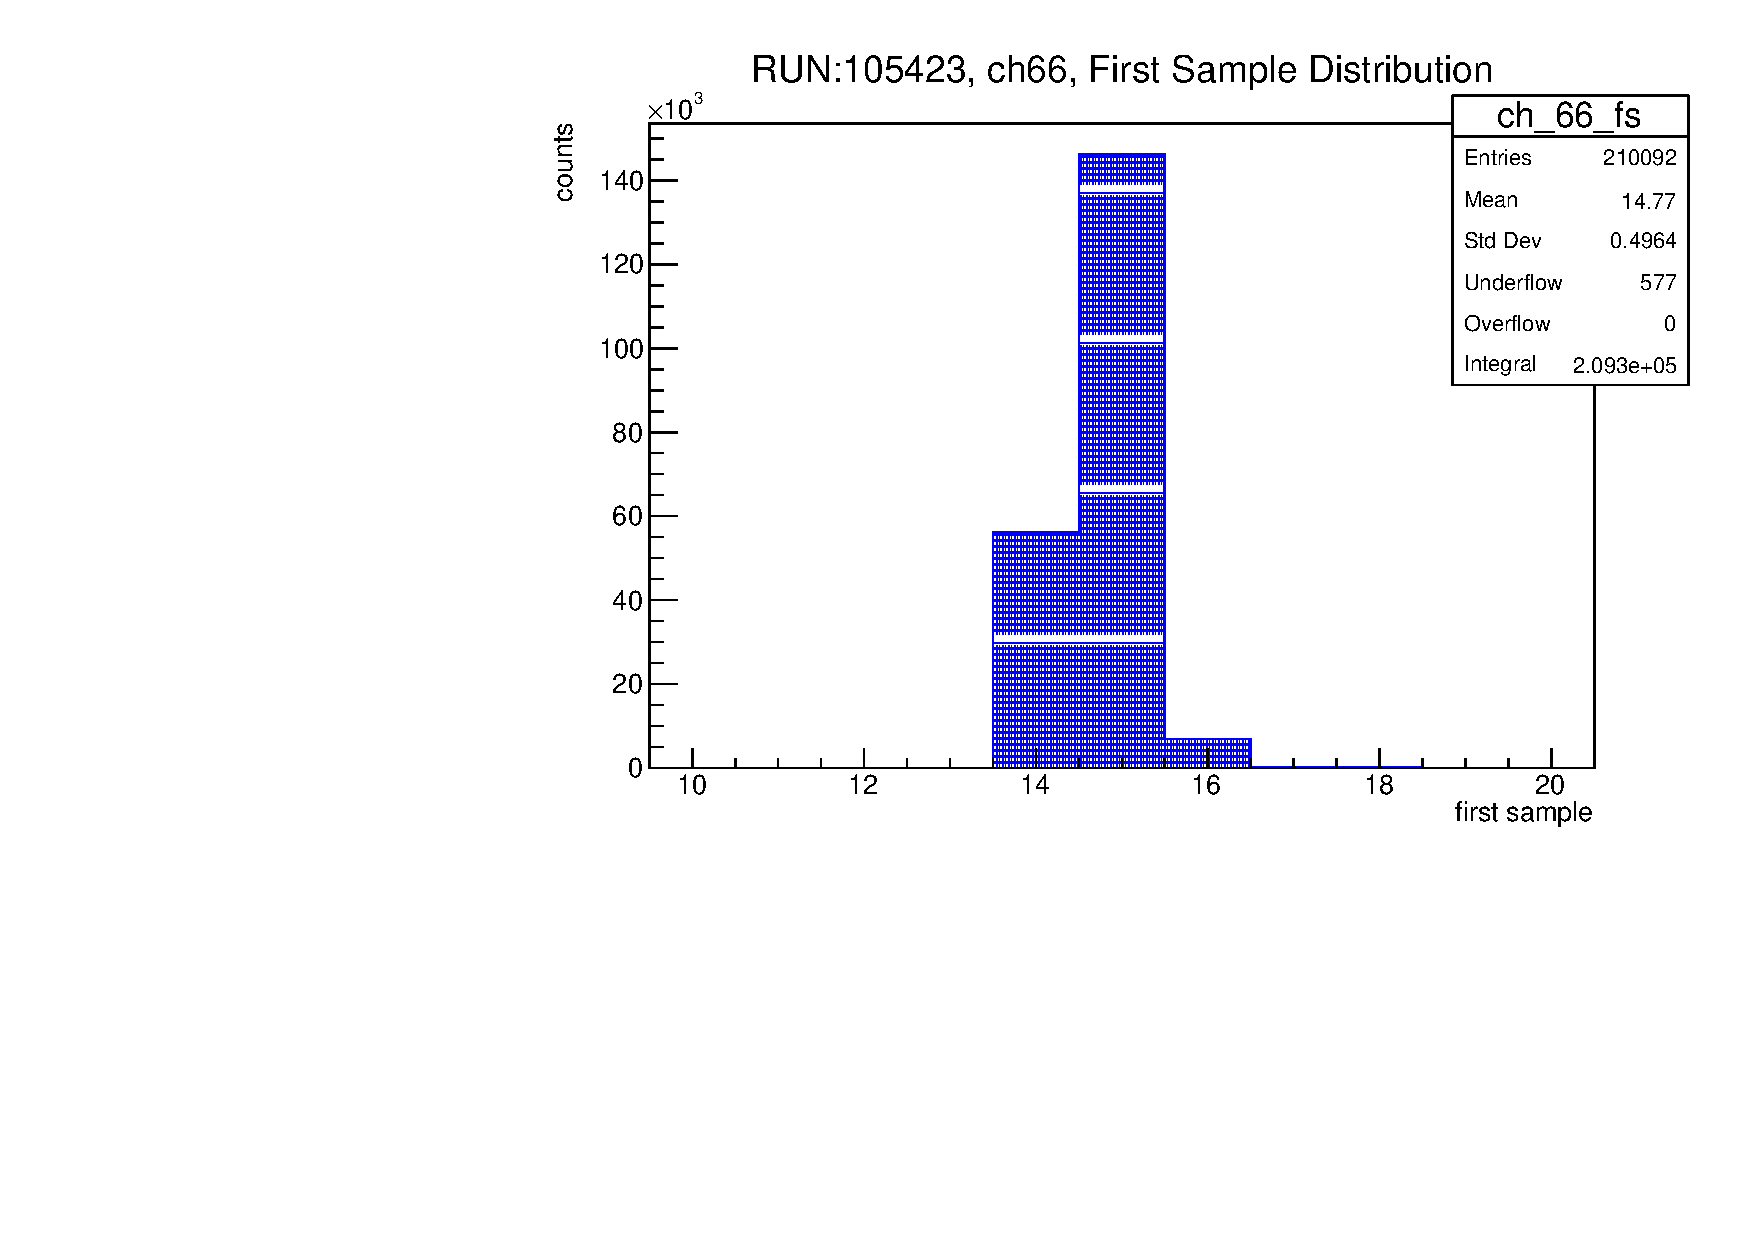
\includegraphics[width=0.65\textwidth]{figures/pdf/fs.pdf}
  \caption{First sample distribution of the waveforms in channel 66.}
  \label{fig:fs2}
\end{figure}

\begin{figure}[!h]
    \centering
    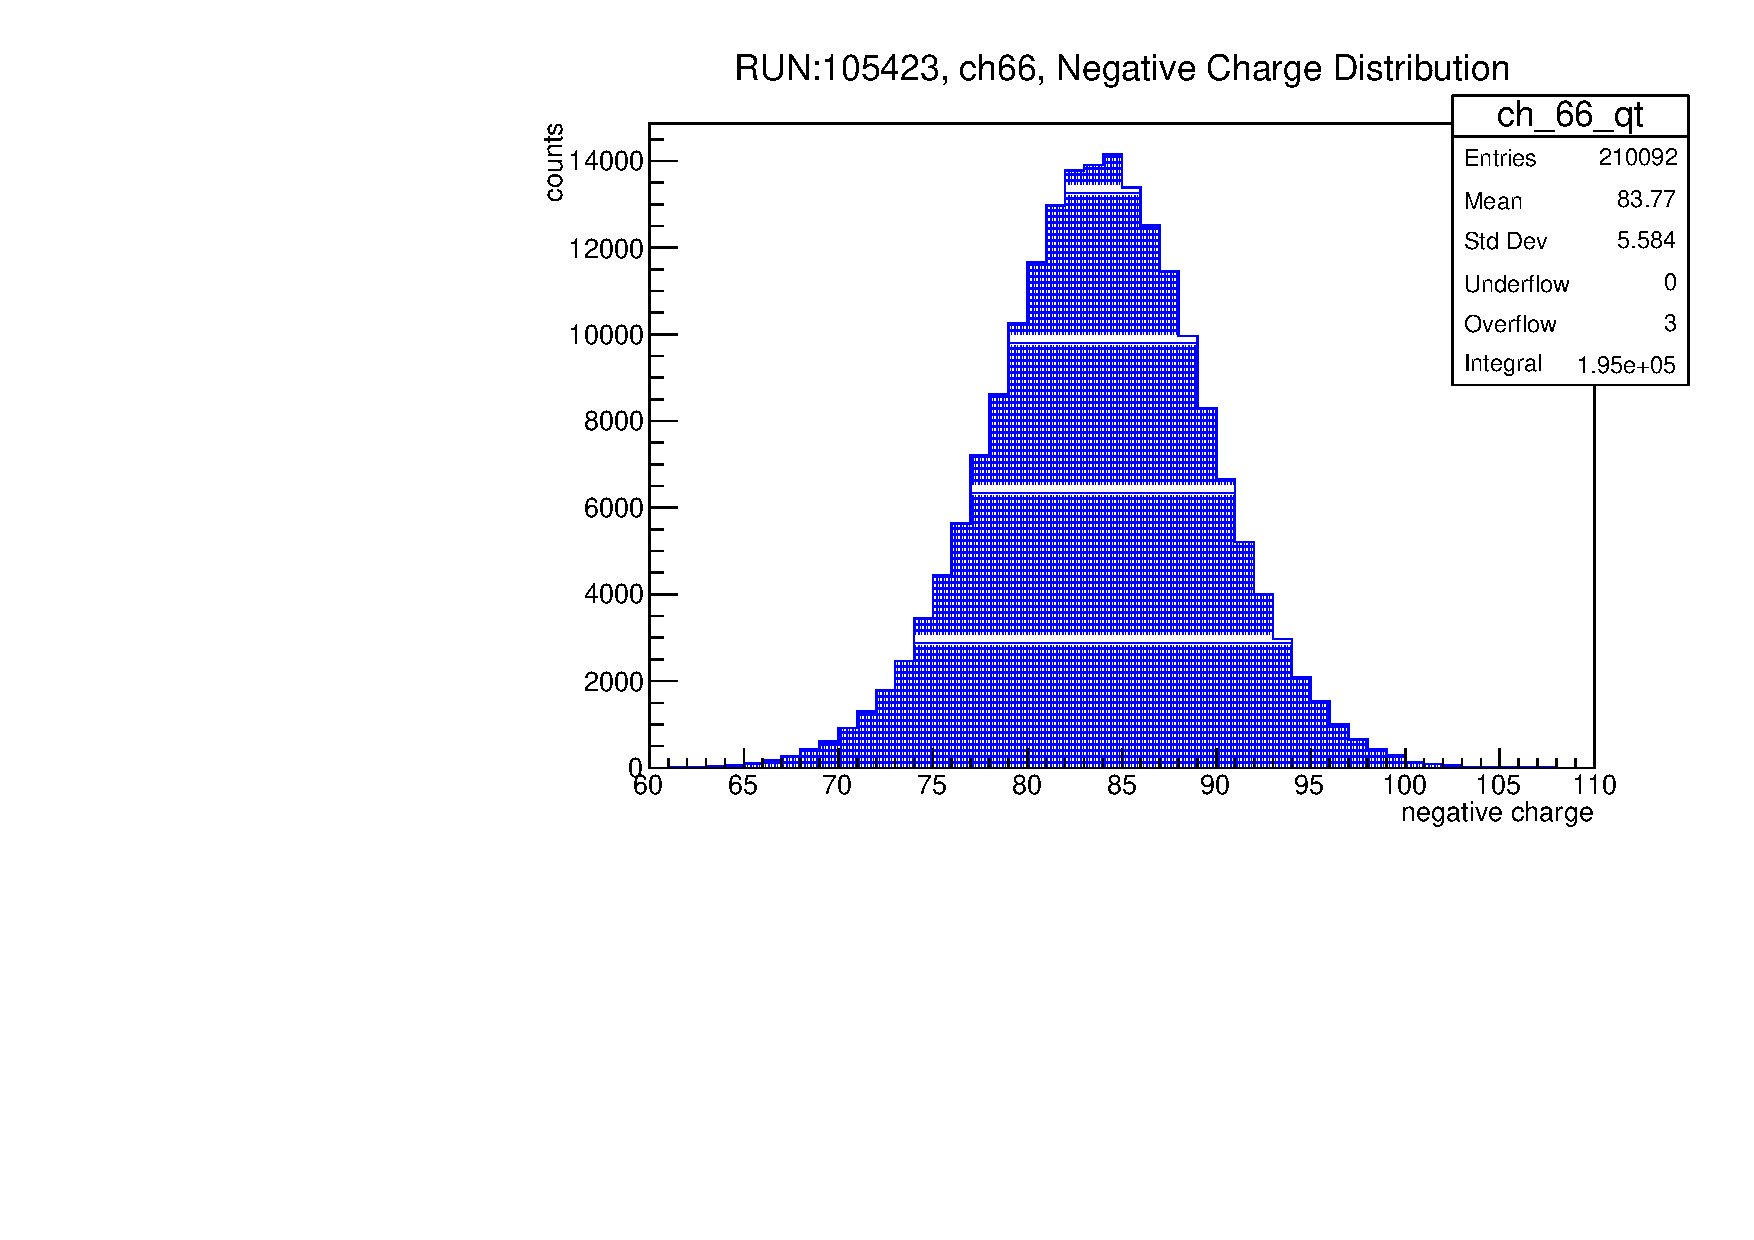
\includegraphics[width=0.65\textwidth]{figures/pdf/negcharge.pdf}
    \caption{Negative charge distribution of the waveforms in channel 66.}
    \label{fig:nch2}
\end{figure}
    
The charge and pulse height distribution exhibit a non-trivial shape. 
Three and two peaks were observed respectively; it was verified that 
these peaks were not correlated with the number of hits. Moreover, a 
correlation between the charge and pulse height peaks was observed, as shown in Figure \ref{fig:chvsph}. 
\begin{figure}[!h]
  \centering
  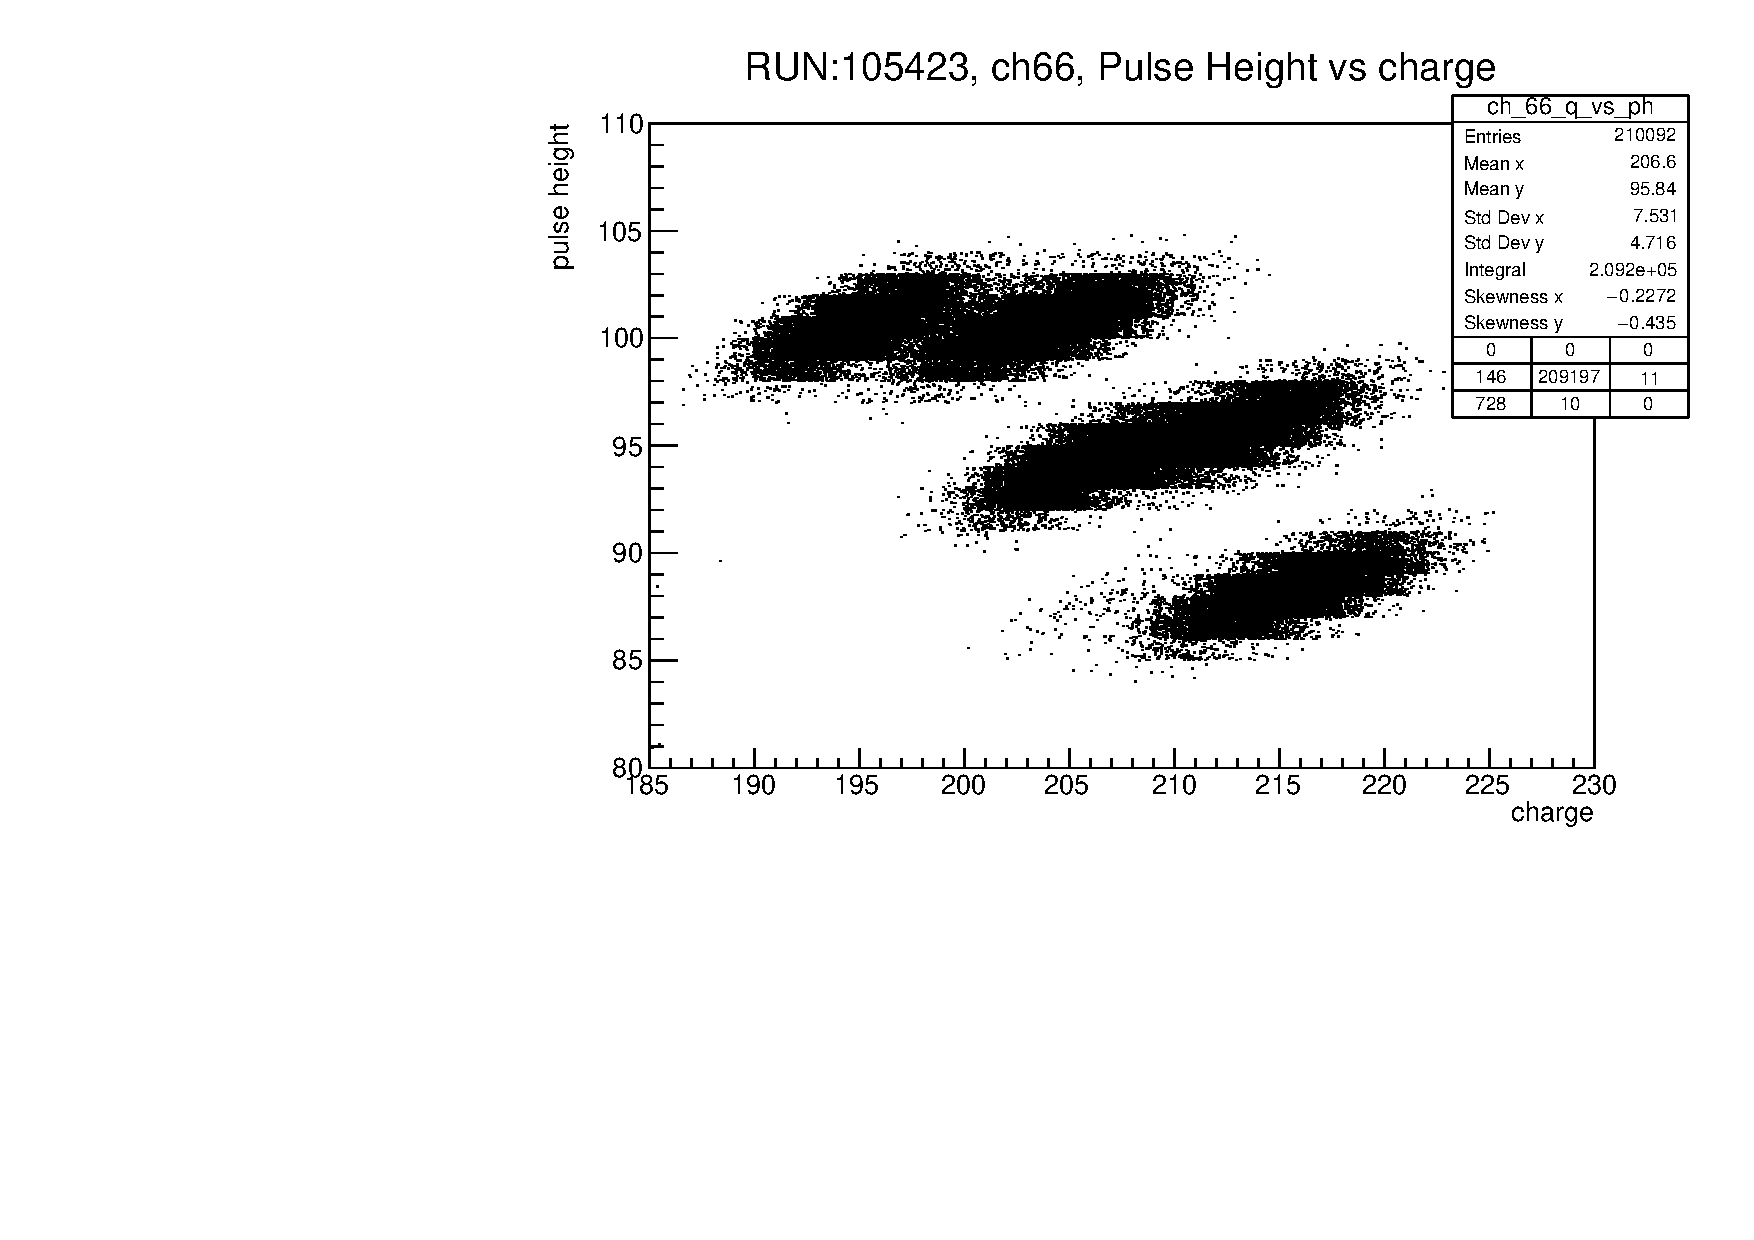
\includegraphics[width=0.65\textwidth]{figures/pdf/phch1.pdf}
  \caption{2D histogram of charge ($x$-axis) versus pulse height ($y$-axis).}
  \label{fig:chvsph}
\end{figure}
To understand the origin of this pattern, the waveform mean sample weighted with the charge 
\begin{equation} 
  s_{mean} = \frac{\sum_i \text{sample}_i \cdot q_i }{\sum_i q_i} 
\end{equation}
distribution was plotted in Figure \ref{fig:smean}. 
This plot shows that the time difference $\Delta s$ (approximately 2 ns) between pulses is less than the bin width, which is 25 ns. 
The next step was to check if $s_{mean}$ could be correlated with charge and pulse height peaks, 
as shown in Figure \ref{fig:chtm} and Figure \ref{fig:phtm}.
\begin{figure}[!h]
  \centering
  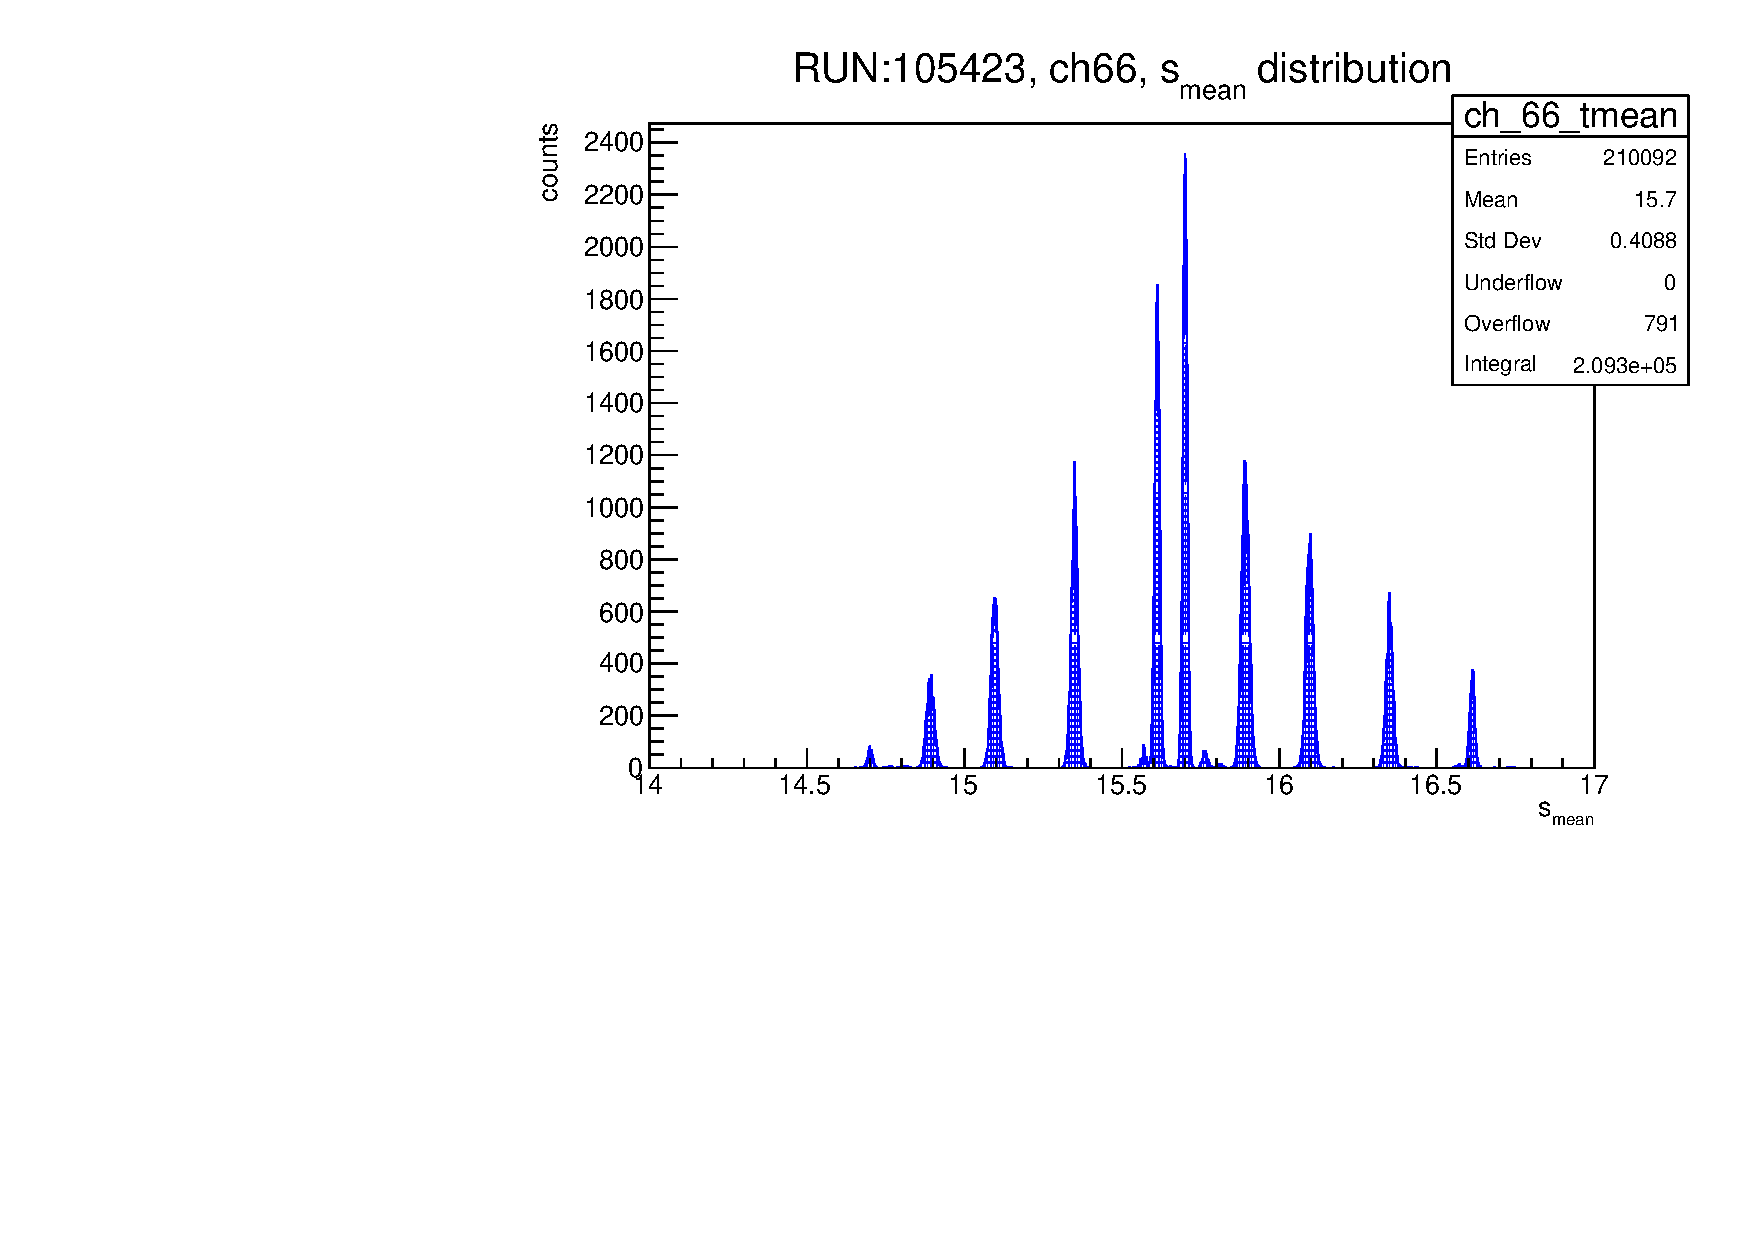
\includegraphics[width=0.65\textwidth]{figures/pdf/tmean1.pdf}
  \caption{Distribution of the waveform mean sample weighted with the charge in channel 66.}
  \label{fig:smean}
\end{figure}
\begin{figure}[!h]
  \centering
  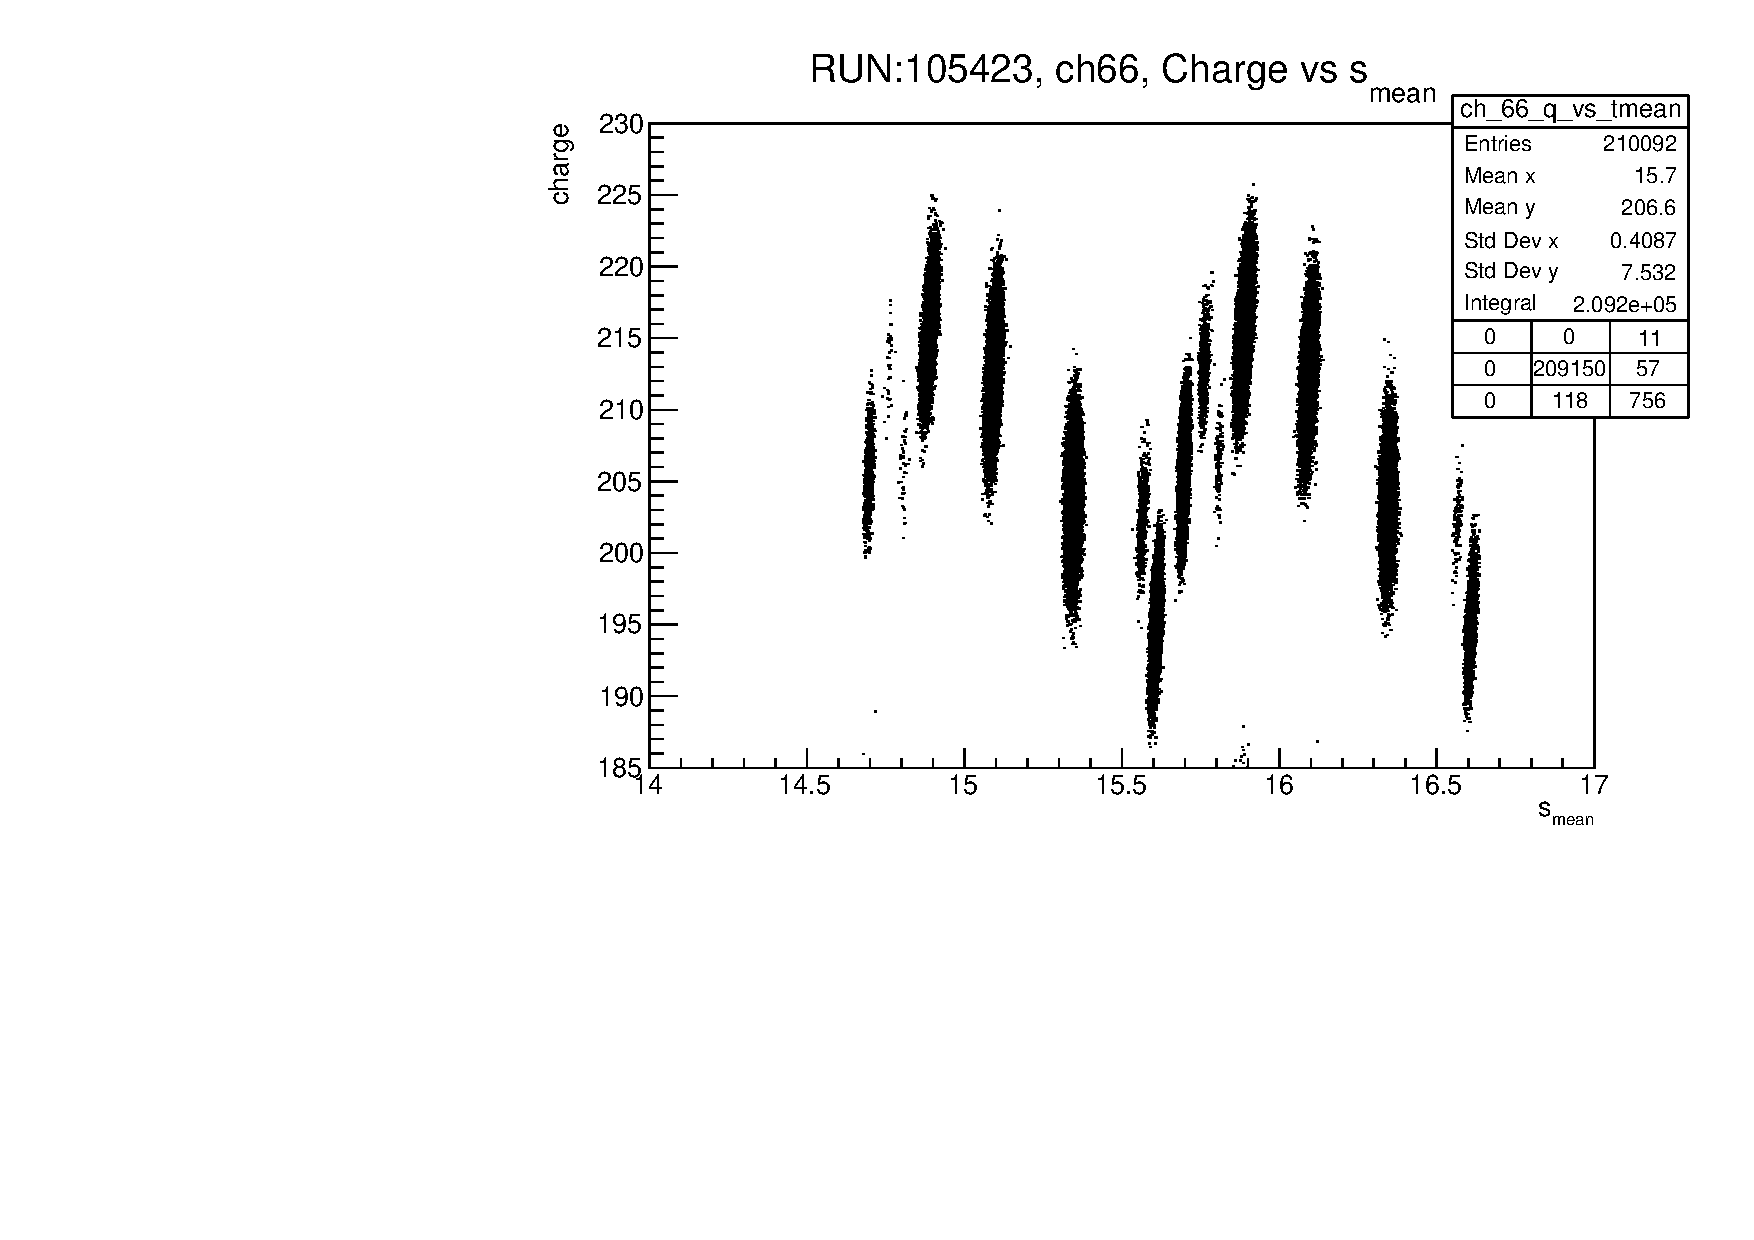
\includegraphics[width=0.65\textwidth]{figures/pdf/chtmean.pdf}
  \caption{2D histogram of $s_{mean}$ ($x$-axis) versus charge ($y$-axis).}
  \label{fig:chtm}
\end{figure}
\begin{figure}[!h]
  \centering
  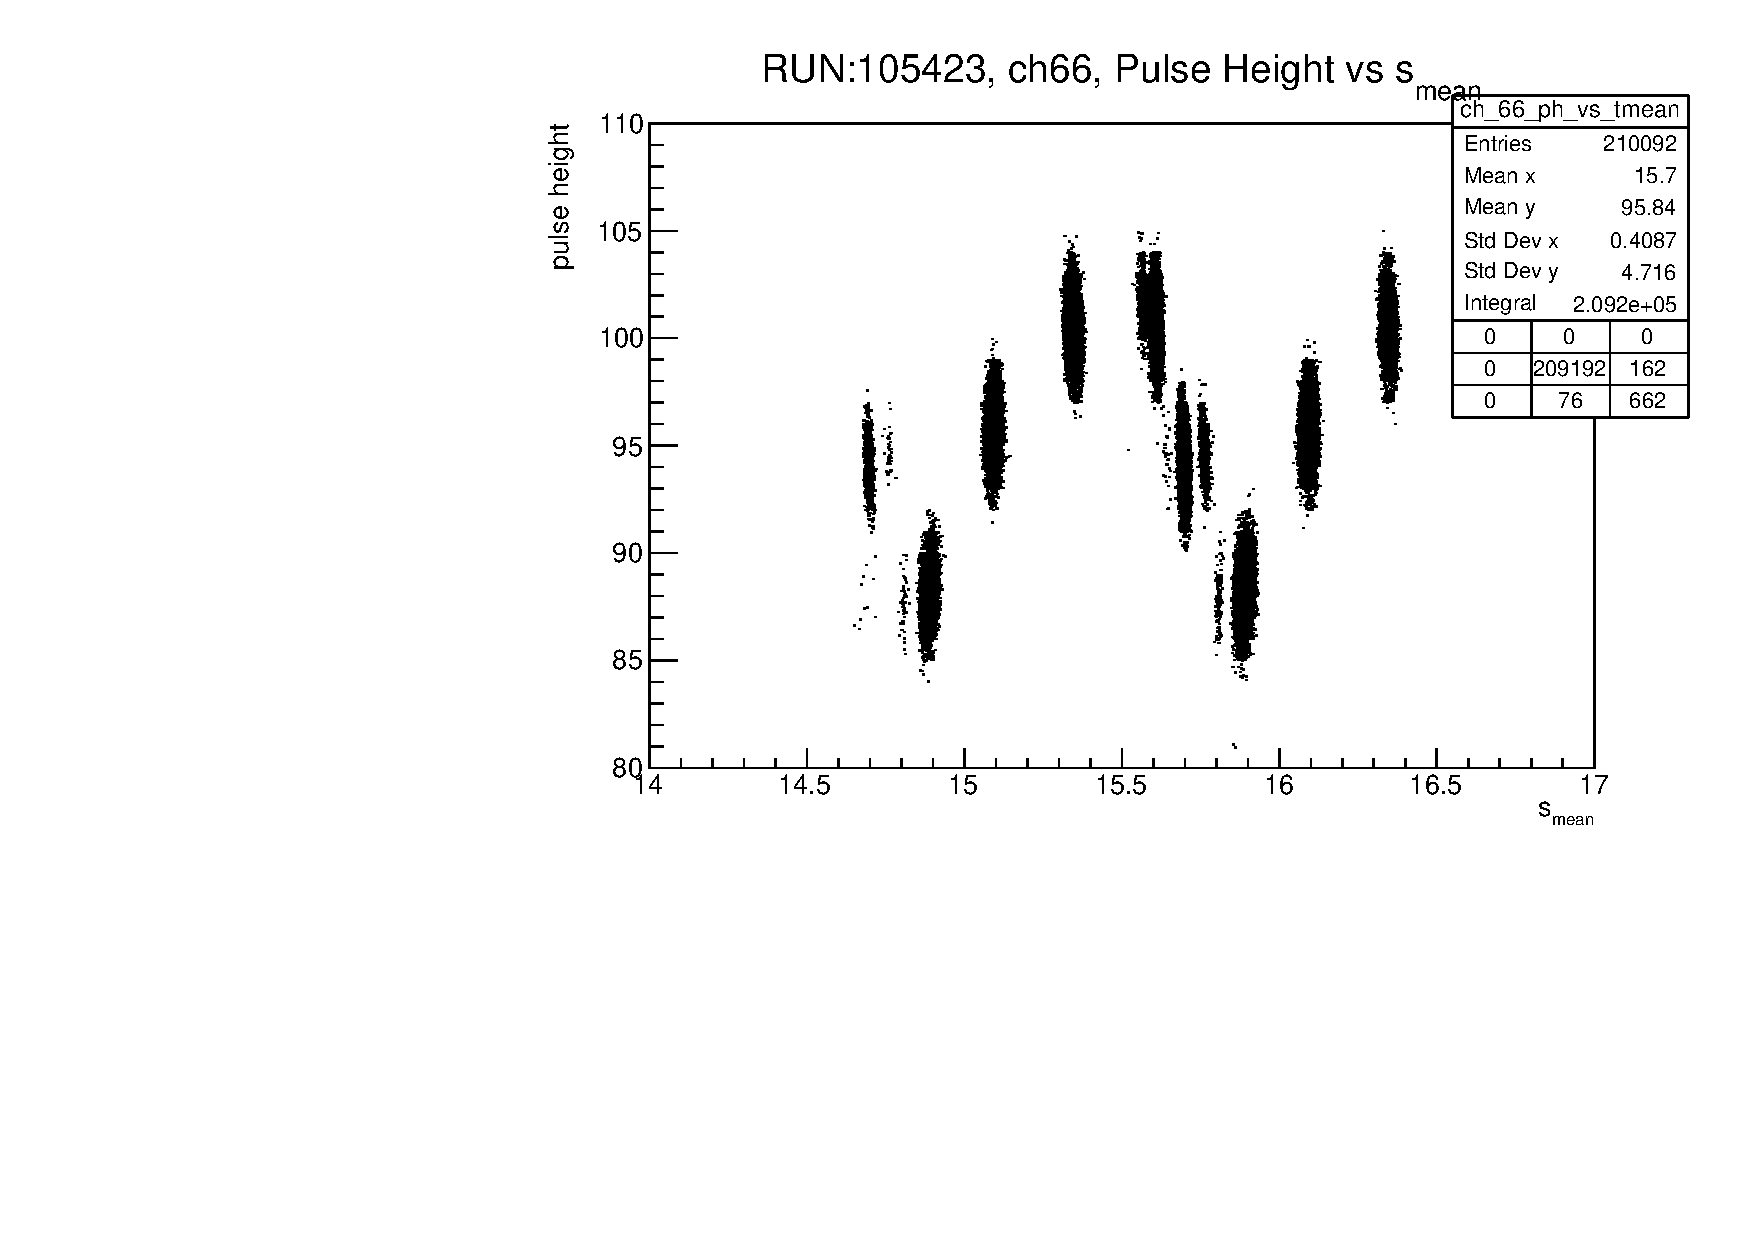
\includegraphics[width=0.65\textwidth]{figures/pdf/phtmean1.pdf}
  \caption{2D histogram of $s_{mean}$ ($x$-axis) versus pulse height ($y$-axis).}
  \label{fig:phtm}
\end{figure}
The pulse height and charge peaks are perfectly correlated with the $s_{mean}$ peaks. 
In particular, few ns of delay between waveforms, correlated with the ADC clock, 
result in three or two peaks in the charge and pulse height distribution. 
These peaks are merely artifacts of the pulser timing shifted with respect to the ADC 
clock and are not problematic. This behaviour was also confirmed with a simple simulation.
The simulation generates two series of triangular pulses, each delayed with respect to the other and models the behaviour 
of the corresponding ADC outputs. The ADC is simulated by partitioning signals into bins and calculating the signal mean within each bin. 
The delay between the two series is shorter than the width of the ADC bins. The output of the simulated ADC consists of square waves 
for each series of triangular pulses. The integrals and maximum values of the square waves over defined intervals are then computed.
The result is shown in Figure \ref{fig:simsim}. The simulation is not intended to replicate reality in its entirety, 
but rather serves as a tool for understanding the correlation between the ADC clock and pulser timing. 
While the simulated charge and pulse height distributions effectively exhibit peaks, they do not precisely 
match the number of peaks seen in Figure \ref{fig:ch1} and \ref{fig:ph2}. Since the ADC begins integration 
at the same time for both pulse series, any temporal shift between waves results in lower or greater waveform values on the 
$y$-axis at identical times. This discrepancy translates into distinct ADC outputs and consequently affects the observed pulse height. 
The same principle applies to the charge. Furthermore, the pulse height peaks exhibit clear distinctions with respect to the charge ones, 
a characteristic also evident in Figure \ref{fig:ch1} and \ref{fig:ph2}.
\begin{figure}[!h]
  \centering
  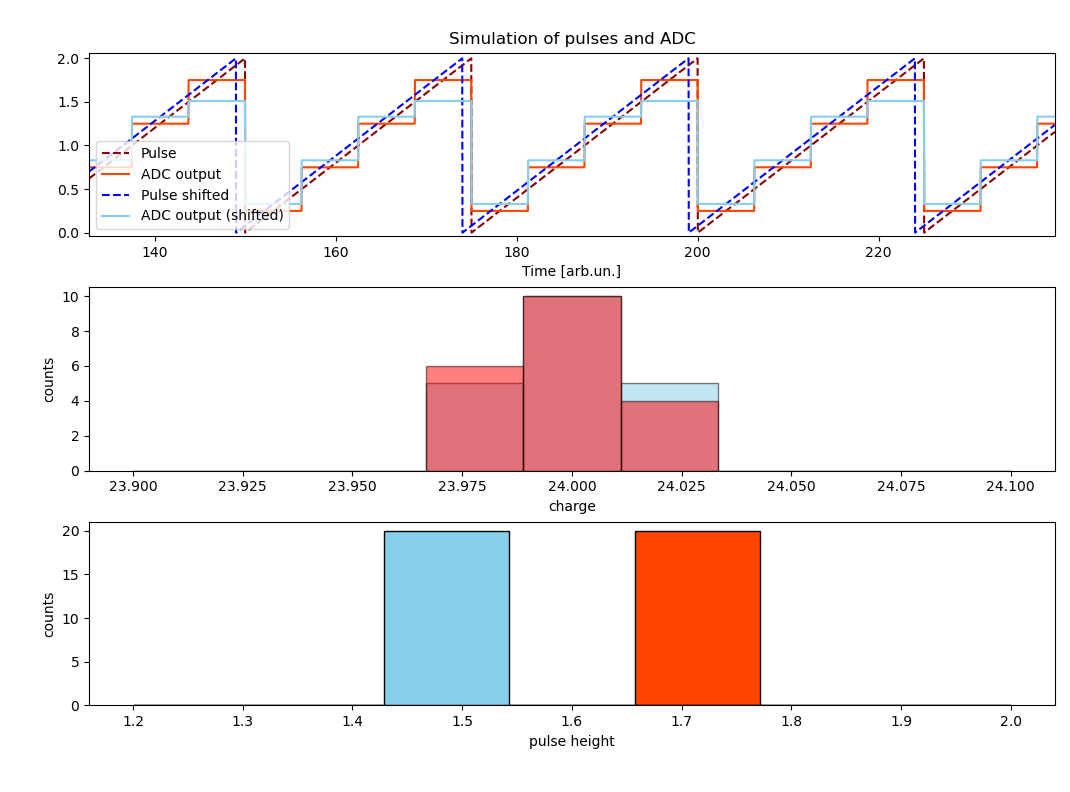
\includegraphics[width=0.85\textwidth]{figures/png/pres.png}
  \caption{Simulation of charge and pulse height distribution behaviour. 
  In the upper plot, triangular pulses representing charge injection waveforms are 
  plotted alongside the square waves from the simulated ADC. The red wave corresponds to the dark red pulses, 
  while the light blue wave corresponds to the dark blue pulses, shifted from the red one. In the central plot, 
  the distribution of charge is displayed, and in the bottom plot, the distribution of pulse height is shown. 
  The light blue distribution corresponds to the light blue ADC, and the same goes for the red one.}
  \label{fig:simsim}
\end{figure}
Lower values of pulse height or charge correspond to inverted waveforms, as mentioned in Sections \ref{nhitvschid} and \ref{wf}, 
or to glitches. In the case of inverted waveforms, the charge value was $\sim$100 and the pulse height $\sim$20, while for glitches, $\lesssim$70 and $\sim$35. 
An example of a glitch is shown in Figure \ref{fig:glitches}. The origin of the glitches is not yet understood.
\begin{figure}[!h]
  \centering
  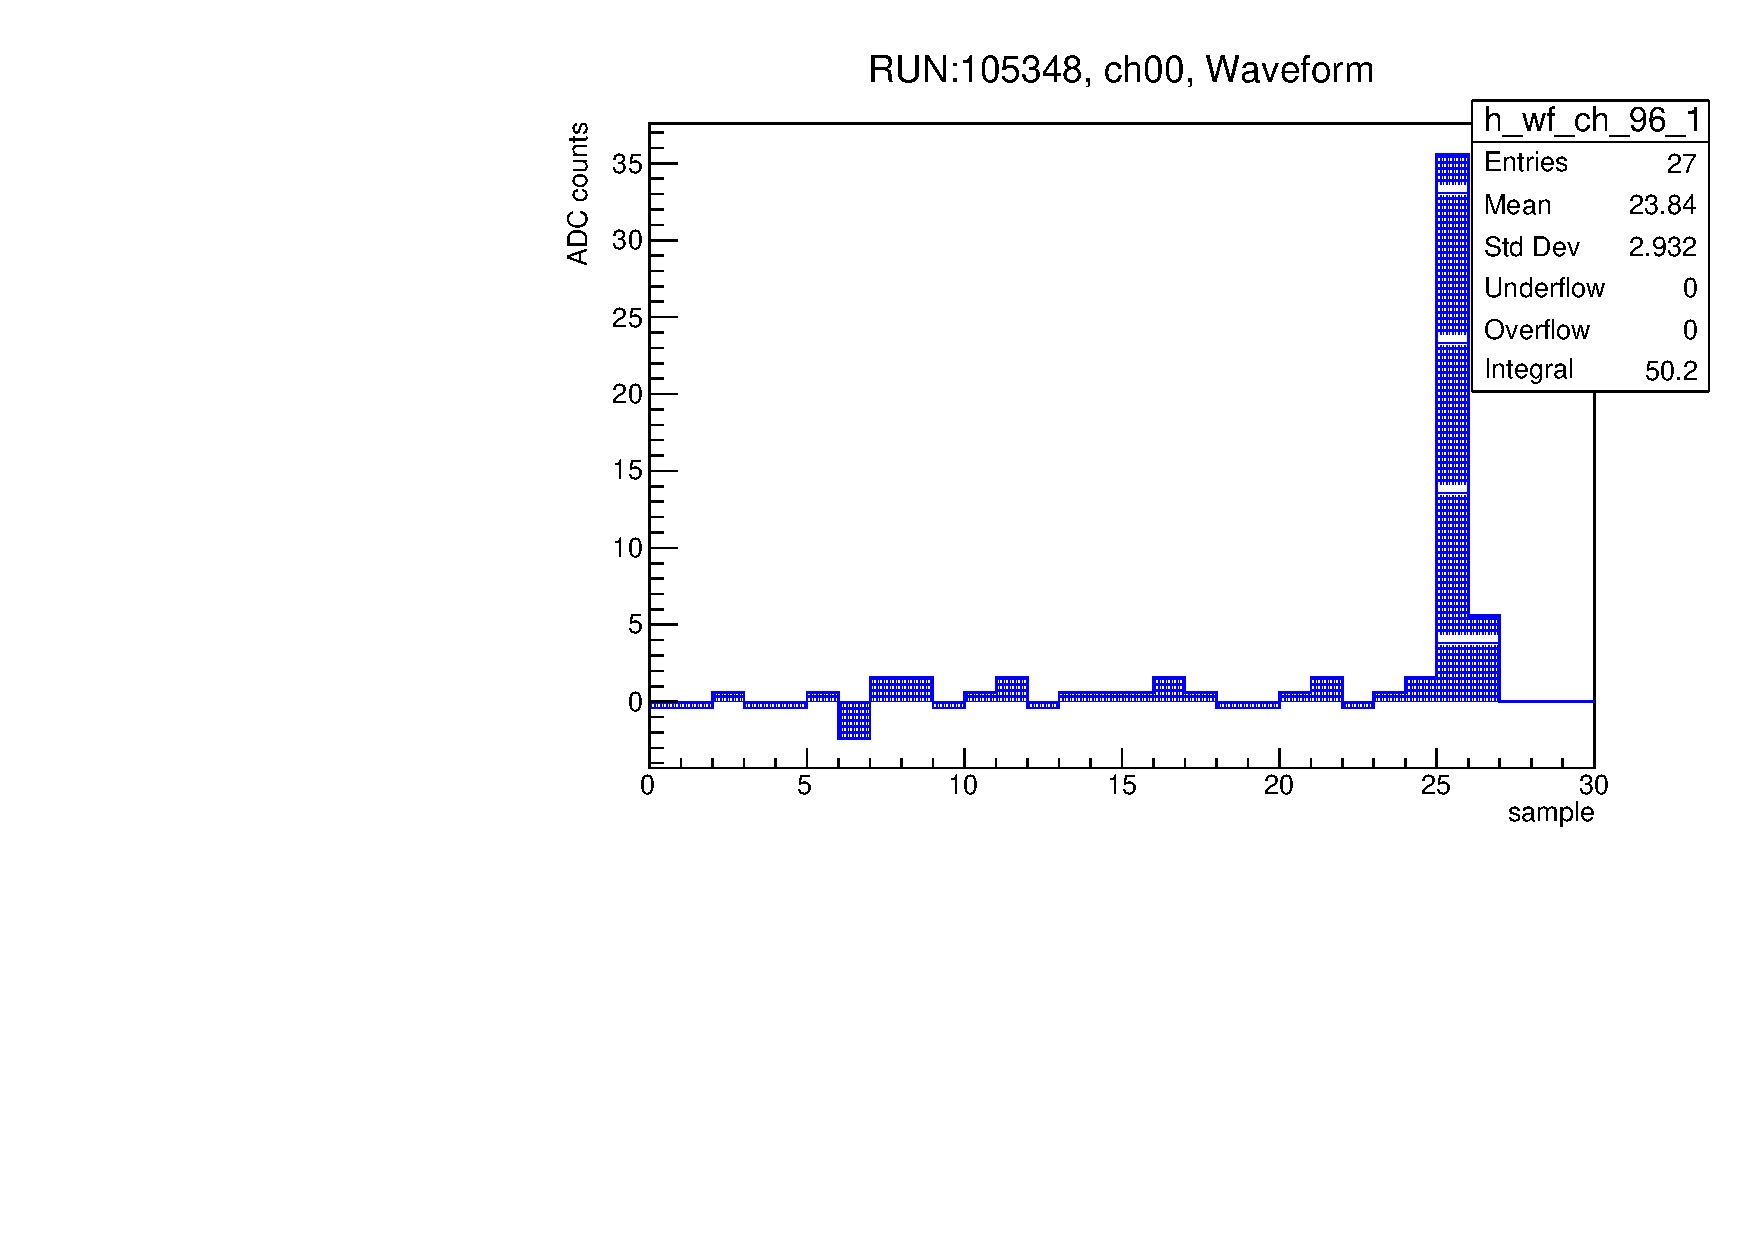
\includegraphics[width=0.65\textwidth]{figures/pdf/glitch.pdf}
  \caption{Glitch waveform of channel 0.}
  \label{fig:glitches}
\end{figure}
Special channels with excessive noise were identified through the charge distribution. 
Figure \ref{fig:noisywf} shows an example of a noisy waveform. 
Since the threshold mentioned in Section \ref{threshold} is 5 ADC counts, charge values for these channels were consistently lower than expected (approximately 10). 
This is due to the fact that only the first sample above 5 was considered as the entire waveform.
To address the issue, the channel voltage threshold was either adjusted or the preamp was replaced.
\begin{figure}[!h]
  \centering
  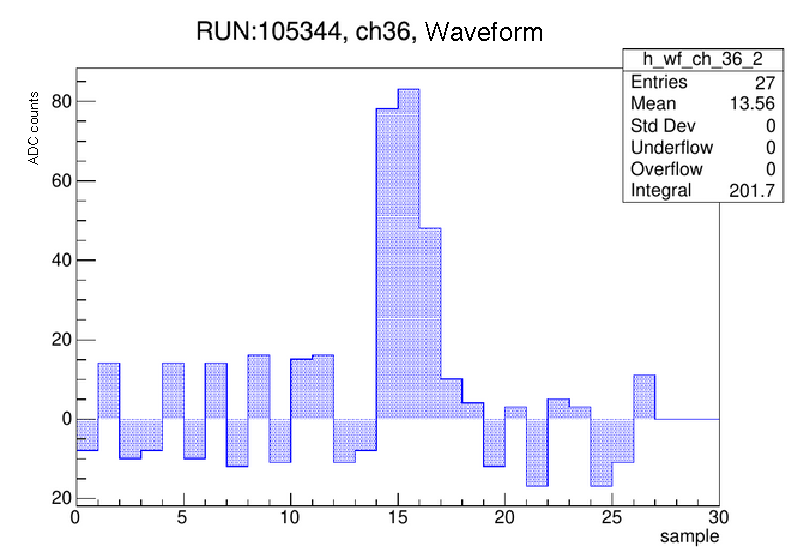
\includegraphics[width=0.65\textwidth]{figures/pdf/noise.pdf}
  \caption{Noisy waveform of the 36th channel.}
  \label{fig:noisywf}
\end{figure}

\subsubsection{Channels response uniformity}
In view of data taking, it was important to find an easy way to identify problematic channels and check the uniformity of channel responses. 
For this reason, plots of charge, first sample, pulse height and baseline means versus channel ID were produced. 
These plots are shown in Figures \ref{fig:blvsch}, \ref{fig:qvsch}, \ref{fig:phvsch} and \ref{fig:fsvsch}. 
The outliers in the plots are due to crosstalk, noisy channels, inverted waveforms and glitches.
\begin{figure}[!h]
  \centering
  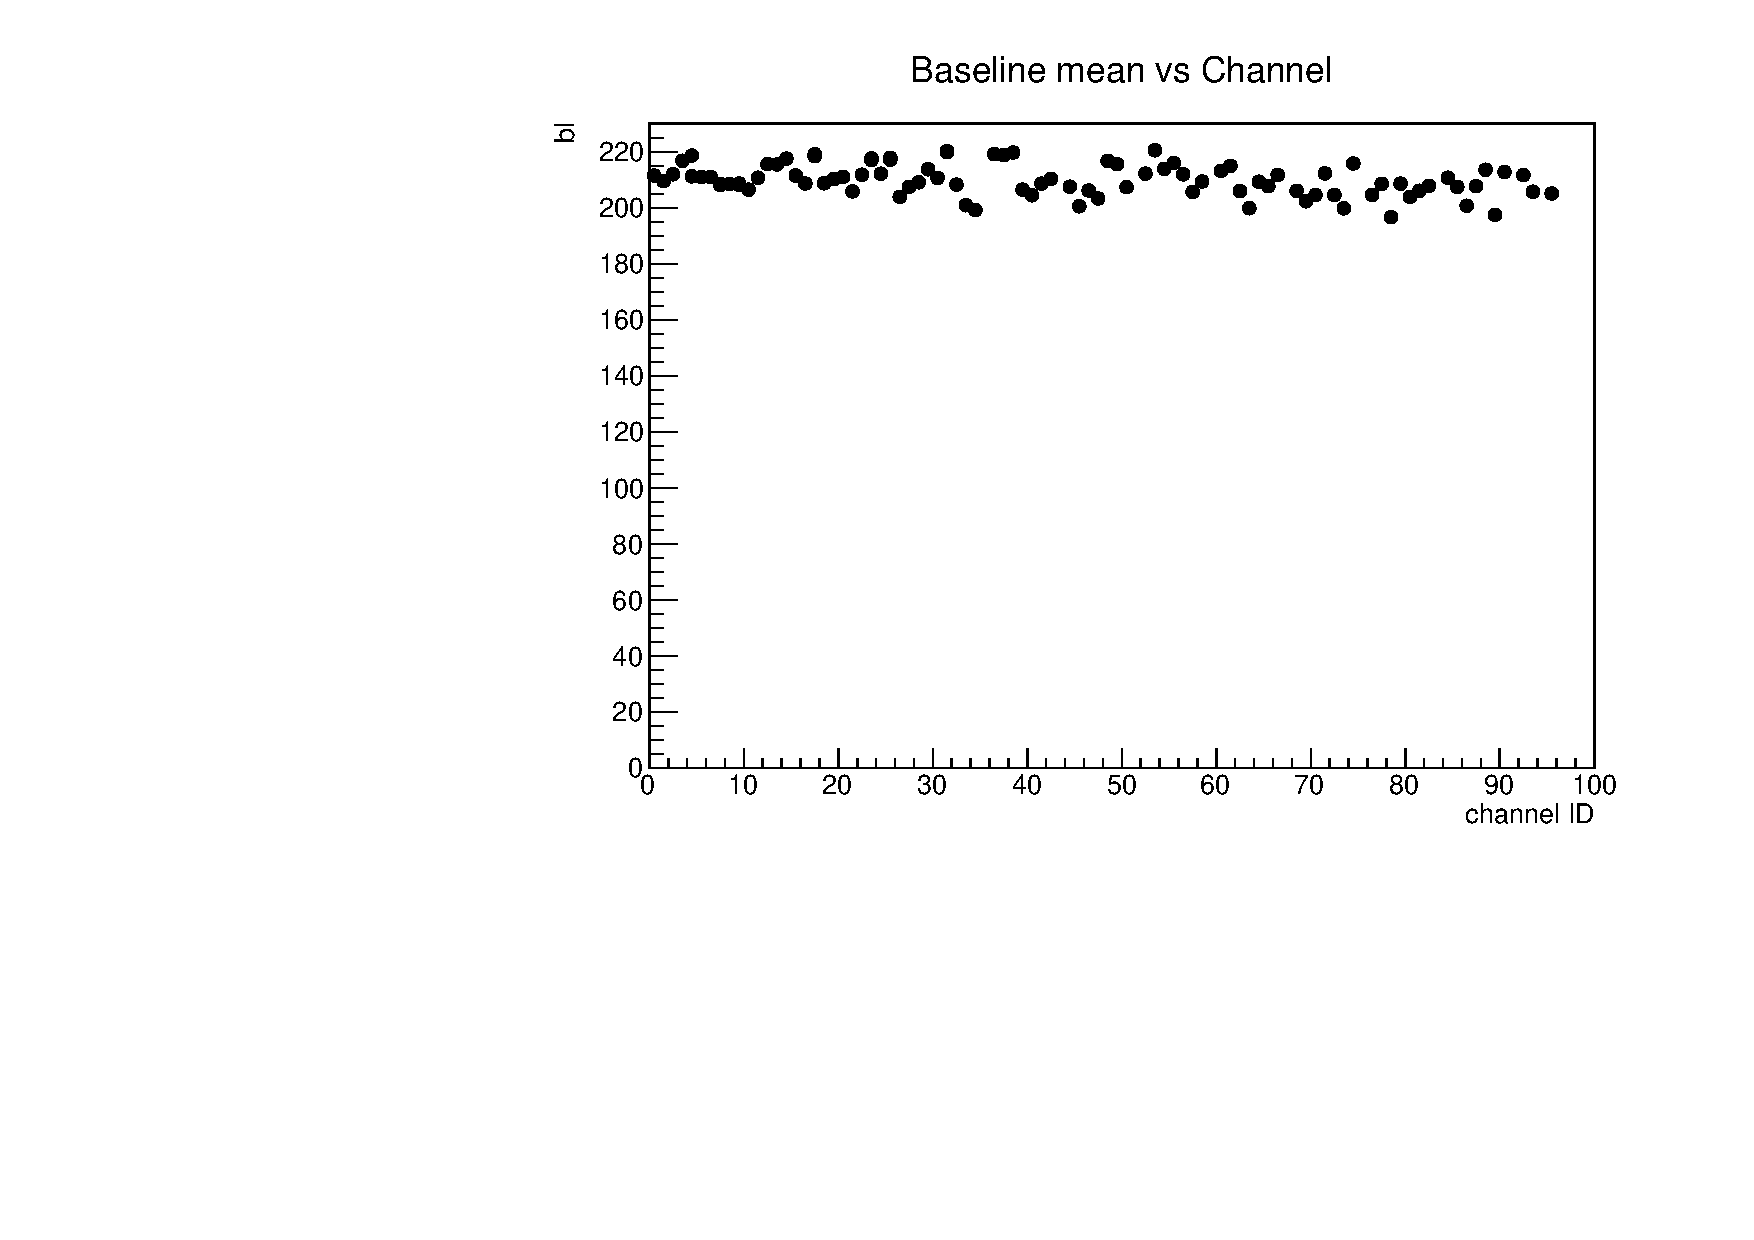
\includegraphics[width=0.65\textwidth]{figures/pdf/bl_vs_ch1.pdf}
  \caption{Baseline mean value versus channel ID.}
  \label{fig:blvsch}
\end{figure}
\begin{figure}[!h]
  \centering
  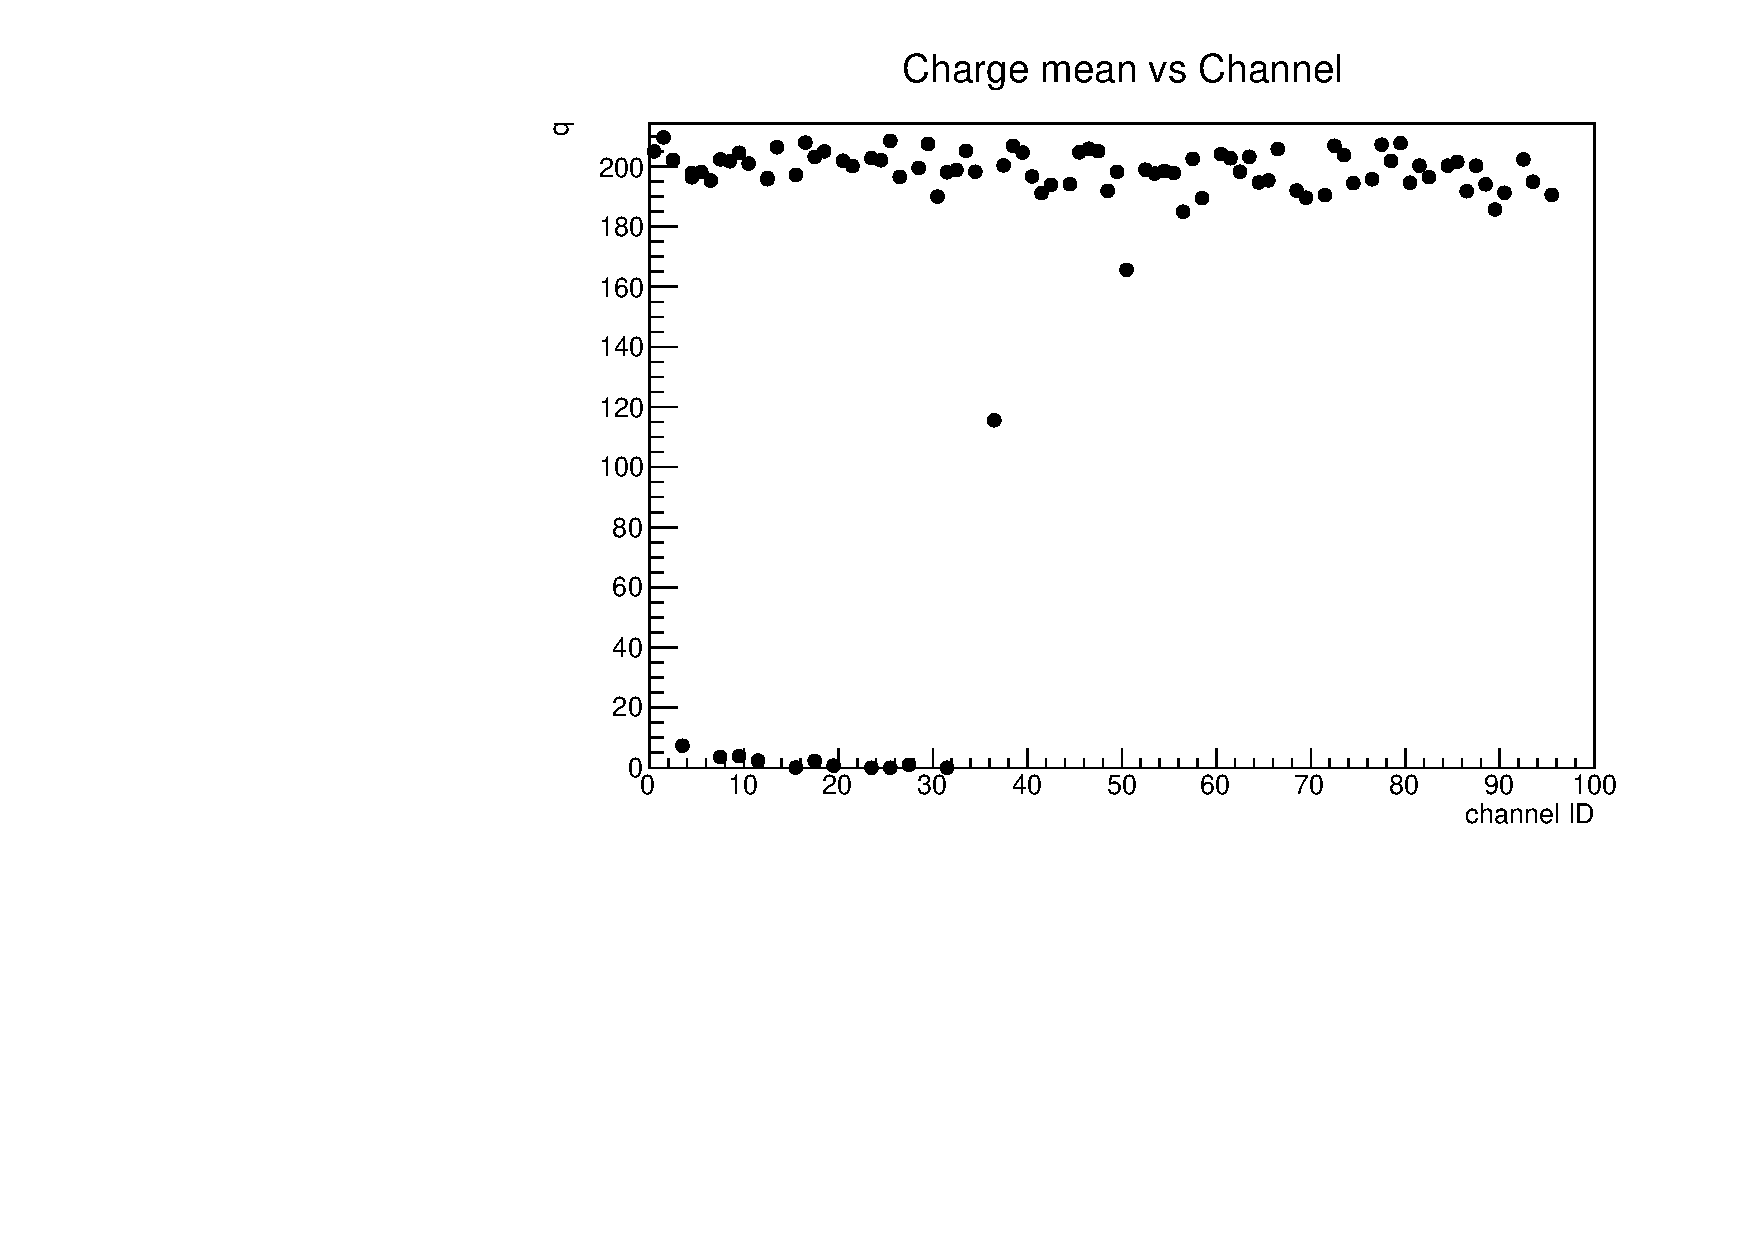
\includegraphics[width=0.65\textwidth]{figures/pdf/q_vs_ch1.pdf}
  \caption{Charge mean value versus channel ID.}
  \label{fig:qvsch}
\end{figure}
\begin{figure}[!h]
  \centering
  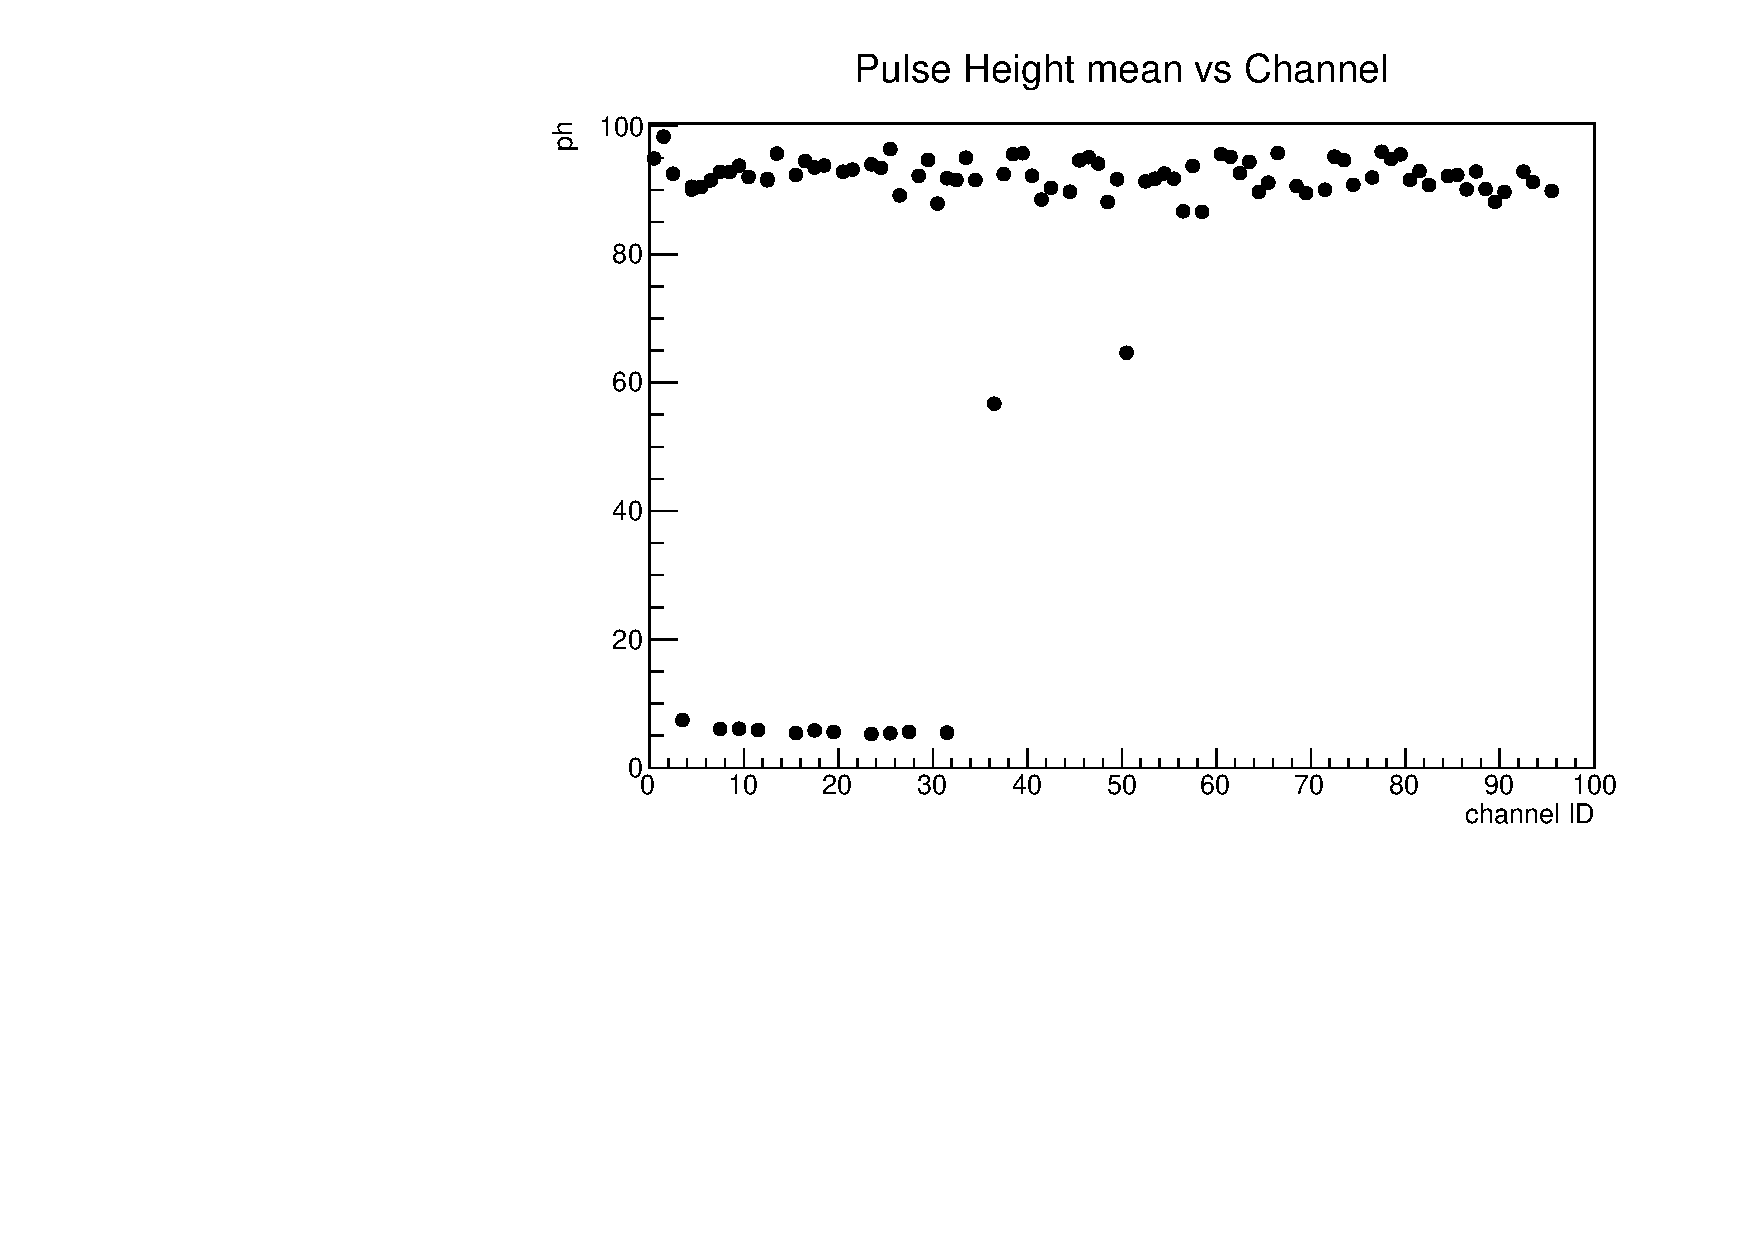
\includegraphics[width=0.65\textwidth]{figures/pdf/ph_vs_ch1.pdf}
  \caption{Pulse height mean value versus channel ID.}
  \label{fig:phvsch}
\end{figure}
\begin{figure}[!h]
  \centering
  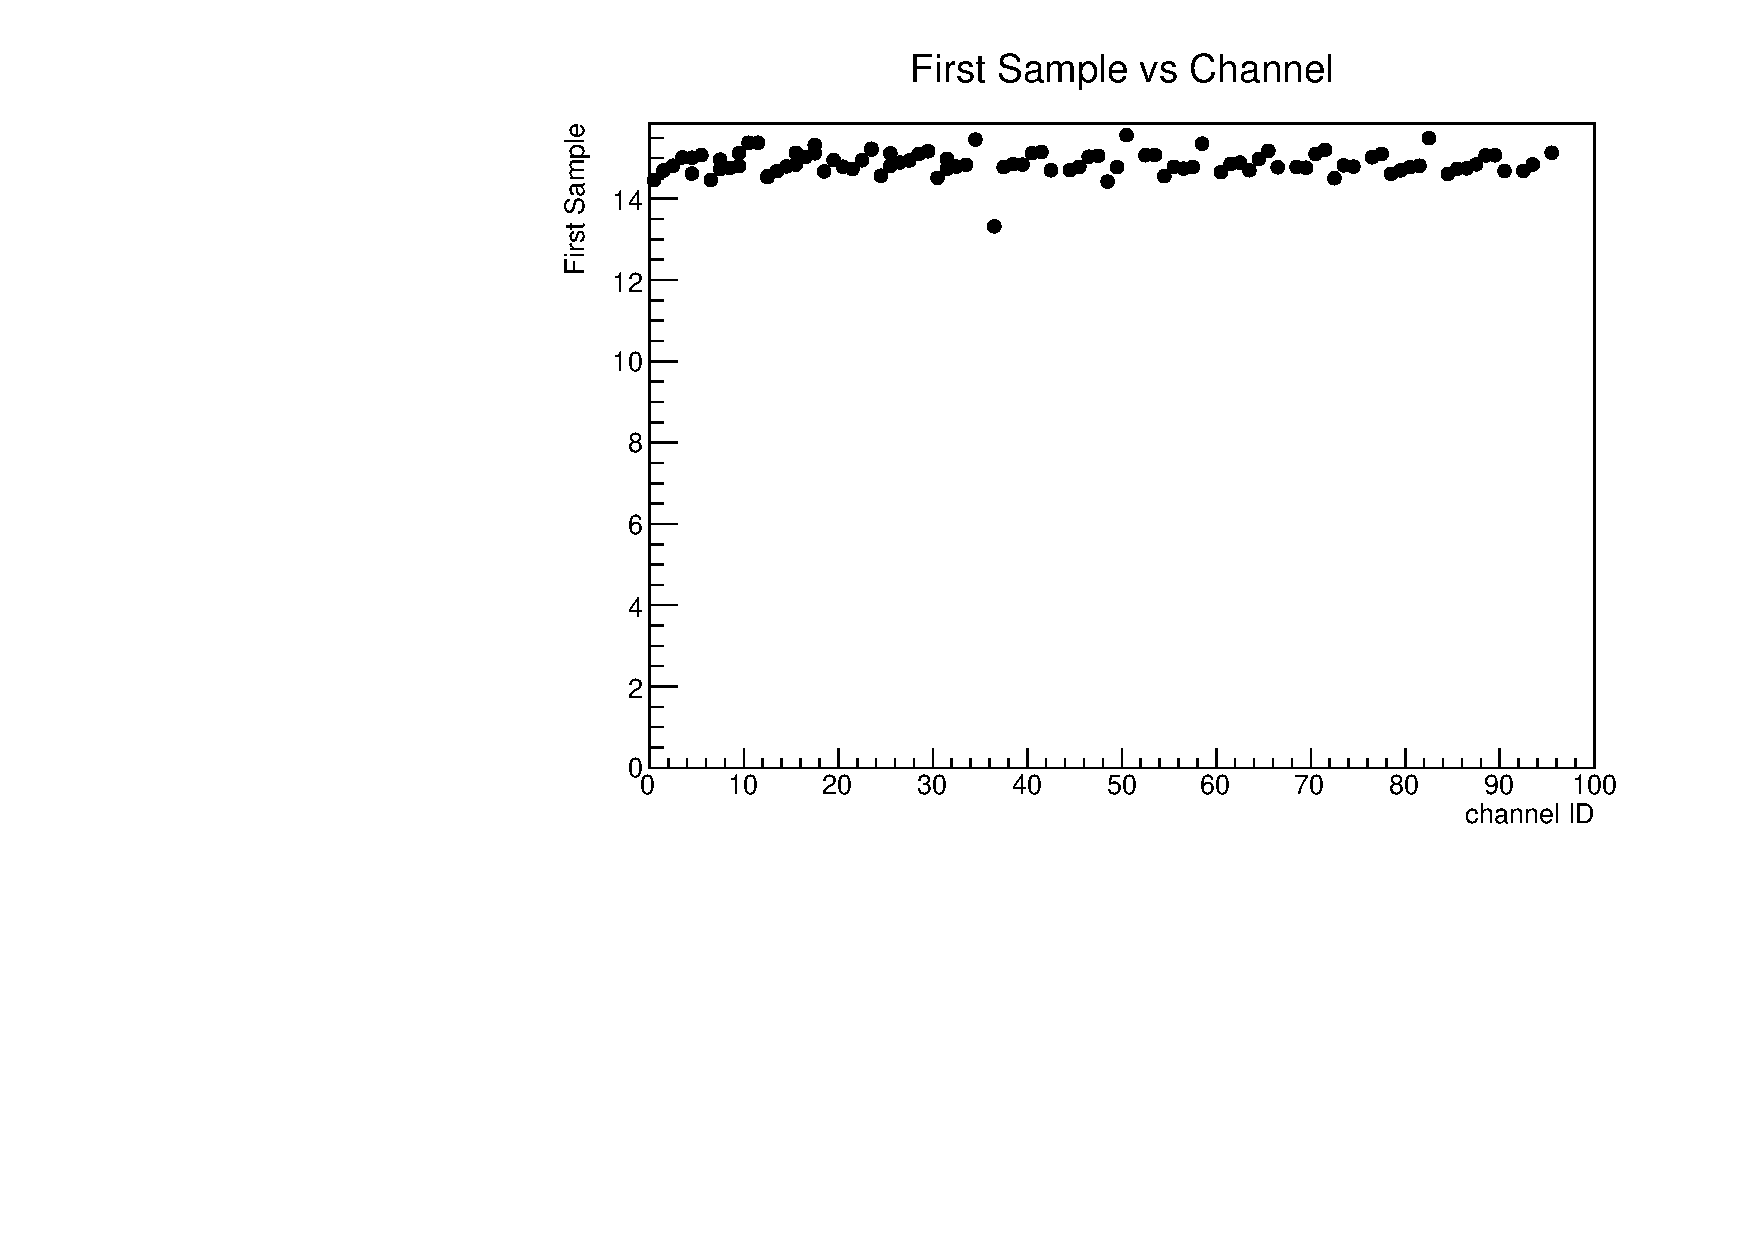
\includegraphics[width=0.65\textwidth]{figures/pdf/fs_vs_ch1.pdf}
  \caption{First sample mean value versus channel ID.}
  \label{fig:fsvsch}
\end{figure}




\iffalse


\section{High rate software testing}
\subsection{Firmware-Based Data Acquisition}
The Mu2e Trigger and Data Acquisition (TDAQ) system collects digitized data from the Tracker, 
Calorimeter, Cosmic Ray Veto and Beam Monitoring components (Stopping Target Monitor and Extinction Monitor) 
and delivers that data to online and offline processing for analysis. It must merge data from $\sim$450 subsystems 
and apply filters to reduce data volume by a factor of 100 before storing it offline. It is also responsible for 
detector synchronization, control, monitoring and operator interfaces. The Mu2e DAQ system uses a $streaming$ readout technique, 
which means that all detector data from the experiment is digitized and zero-suppressed in their respective Front End Electronics 
(FEEs) before being transferred. This strategy results in a high data flow in the DAQ system while providing greater flexibility in data selection and analysis.
\subsubsection{Expected rate}
The data-taking periods will be divided into two modes: on-spill and off-spill. The on-spill mode includes periods when 8 GeV 
proton bunches are colliding with the production target. The off-spill mode includes all other periods, such as between bunches, calibration periods and commissioning.
According to section \ref{accel}, it is possible to estimate the on-spill event contribution as follows:
\begin{itemize}
    \item $\frac{43.1 \text{ ms (time of one spill)}}{1695 \text{ ns (digitization time)}}$ = 25,000 pulses per spill;
    \item 8 (number of spills) $\times$ 25,000 (pulses per spill) = 200,000 on-spill events per cycle;
    \item $\frac{200,000 \text{ (on-spill events per cycle)}}{1.4 \text{ s (cycle time)}}$ = 145,000 on-spill events per second.
\end{itemize}
%di questi 1.4s, 1.055s si riferisce all'offspill e 0.4s all'onspill.
Meanwhile, the off-spill event contribution is:
\begin{itemize}
    \item $145,000 \text{ (on-spill events per second)} \times 0.4 \text{ s (off-spill time)}$ = 58,000 off-spill events per cycle;
    \item $\frac{58,000 \text{ (off-spill events per cycle)}}{1.4 \text{ s (cycle time)}}$ = 41,000 off-spill events per second.
\end{itemize}
The total input rate will be 186,000 events/s. %Hz
There is a mean factor 100 of trigger, so 1800 events/s.
The detectors will generate $\sim$150,000 Byte per event of zero-suppressed data, for an average data rate of $\sim$90 GB/s when beam is present. 
To reduce DAQ bandwidth requirements, this data is buffered in Readout Controller (ROC) memory during the spill period and transmitted to the 
DAQ over the full supercycle for an average data rate of $\sim$28 GB/s.
The total input is 150,000 Byte per event $\times$ 1800 events/s that is 270 MB/s.
\subsection{ARTDAQ}
\section{Data flow testing}
\fi

 %(1695 ns), that is 90 GB/s and there is a buffering factor of 0.4/1.4, that makes 28 GB/s.


%In Figure \ref{fig:linktodaq}, the general design of the Mu2e DAQ system is shown.
%\begin{figure}[!h]
%\centering
%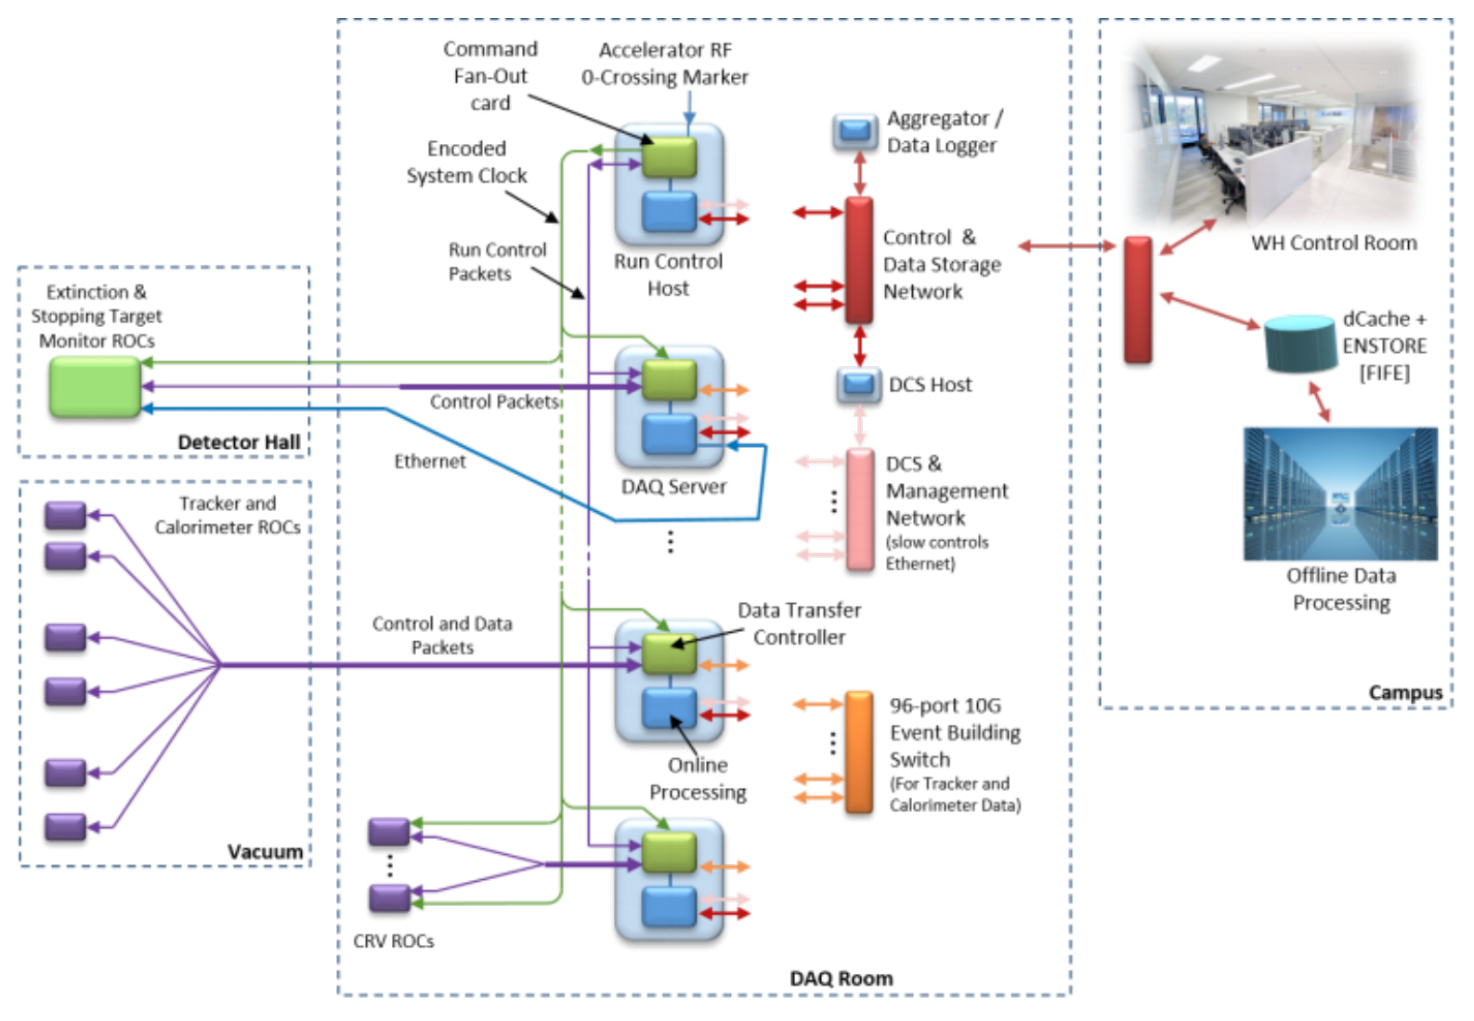
\includegraphics[width =0.65\textwidth]{figures/png/Screenshot_20240206_144803.png}
%\caption{Mu2e DAQ Architecture.}
%\label{fig:linktodaq}
%\end{figure}
%The left blocks represent the Readout Controllers (ROCs) in different detectors. The center 
%lock houses the DAQ system's online components, which include the Run Control Host, 40 DAQ servers, 
%the Detector Control System (DCS) and the Event Building Switch. The Run Control Host receives beam status 
%and timing information from the Accelerator Controls network and operator commands from the remote control room. 
%The Detector Control System (DCS) is the window onto the status and health of the Mu2e detector. The Event Building 
%(EVB) function combines these subsets to form a complete detector data set for analysis by an online processor, Ref. 
%\cite{bartoszek2015mu2e}. Event building is typically done in a switching network to sustain high rates. The right block 
%houses the DAQ system's offline components, which are $\mu$sed for data storage and processing. During an active spill 
%(the first approximately 43 ms of the 48 ms bunch extraction cycle outlined in Chapter \ref{accel}), the experiment receives
% RF Zero-Crossing Markers from the Accelerator that are synchronized to the 1695 ns proton pulse cycles (the event windows). 
% Based on these markers, the Command Fan-Out (CFO) module within the Run Control Host generates a 40 MHz system clock and encodes 
% Event Window Markers (EWMs) in the system clock to indicate the start of the event windows. The CFO then sends the encoded system 
% clock, along with run control packets, to Data Transfer Controllers (DTCs) in the DAQ servers. The DTCs\footnote{The Mu2e Data 
% Transfer Controller (DTC), Ref. \cite{ryan} takes data from various Read-Out Controllers and may conduct event construction and 
% data preprocessing. The DTC module connects a maximum of six ROCs to the Trigger and Data Acquisition (TDAQ) servers, 
% which execute the TDAQ online software framework.} then transfer the encoded clock to the detectors' ROCs, where the EWMs 
% are recovered with fixed delay relative to the original RF Zero-Crossing Markers and $\mu$sed in the local ROCs to discriminate 
% data acquired during consecutive event windows. The Tracker generates a DDR3 memory address at the beginning of each event window. 
% The relevant memory area is designated to hold Tracker hits received during that event window. Data requests trigger data readouts 
% from the ROCs to the DAQ system. The Data Requests are modifiable through the CFO as described by the Run Plan, although they are 
% initially given to the Tracker and Calorimeter ROCs via the DTCs following each event window.
% Each tracker hit is composed of a data packet having a fixed length of 128 bits (16 bytes):
 %\begin{itemize}
  %   \item 16 bit header - it contains information as a packet header, a channel identifier to 
   %  specify the channel so the ROC can assign the hit to a wire number and a packet checksum;
    % \item 16 bit - TDC left straw end;
    % \item 16 bit - TDC right straw end;
    % \item 8$\times$10 bit ADC.
% \end{itemize}






%A packet of 128 bits can be transferred every 640 ns (200 Mbps).An additional 32
%bits must be added as an end-of-file marker after the data $\mu$spill hit data is buffered.
%The ROC-to-DAQ connection is made via fiber optic links arranged in rings, with multiple ROC per ring, as shown in Figure \ref{fig:linktodaq}. 
%This is possible since a single optical link can handle 2.6 Gbps, while the ROC output is around 230 Mbps. This value comes from the fact that the 
%highest rate for any 4 straws group (corresponding to one digitizer data line to the ROC) is 240 kHz or 30 Mbps (at 128 bits/hit) and the Main Injector 
%supplies Mu2e beam only 32\% of the time. The ROC monitors slow control variables and controls panel operations too.


